\documentclass[]{article}
\usepackage[margin=0.5in]{geometry}
\usepackage{graphicx}

%opening
\usepackage{wrapfig}
\usepackage{bookmark}
\bookmarksetup{
	numbered, 
	open,
}

\begin{document}



\section{Different Greedy Methods- I Named them results based on folder}
(Note:2 exponents are redundant if they're similar to the third decimal place, default factor is 2.)\\
$\textbf{results}$ - exits if number of functions is $30$ or KL-Divergence is less than $1e-6$ or redundancies are found or the next set of choices for n+1 basis functions is not better than current n basis functions. \\
$\textbf{results\textunderscore original}$ - same as results except completely Ignores if redundancies occurred but it does record that it did find them.\\ THe point of this method was to see if "one can get out of being redudant if we ignore their presence". Answer is no.\\
$\textbf{results\textunderscore redundancies}$ - same as results except if redundancies are found and they have better error (KL diverg.) then it reverts back to the smaller/condensed parameters. If not, it goes back to n basis function and tries again with a new factor. If redundancies are found 5 times in a row, it exits.\\ The point of this method was to see if "changing the factor gives different answer" and "use redudancies to refine our parameters and continue greedy from that "condensed" parameters".

\section{How each Element Exited Based on Method} 
No method exited because it reached 30 basis functions or because it found five redundancies in a row. 
\paragraph{results - }Format: element name (number of basis functions)-\\ Exited because Redudandcies Were Found: he(8), li(8), b(13), be(11), c(10). \\
Exited because objective function was small: n(10), o(8), f(8), ne (8). 

\paragraph{results\textunderscore original} -\\
Exited because next n+1 basis func was not better: he(13), li(10), be(12), b(14), c(21) \\
Exited because objective function was small: n(10), o(8), f(8), ne(8).

\paragraph{results\textunderscore redundancies}- \\
Exited because next n+1 basis func was not better: he(7), li(8), be(9), b(10), c(20) \\
Exited because objective function was small: n(10), o(8), f(8), ne(8).\\
Exited because 5 redudancies were found in a row : None $\Rightarrow$having an adaptive factor here is useless\\ \\ 
General Conclusion is small elements tend to exit by not finding better choices and converges mostly around 8 functions.

\section{Redundancies Information Format: Element(Numb.of Basis Functions, Numb. after removing redundancy)}
\paragraph{results-}Note:exits if redun. He(8, 7), Li(8, 7), Be(11, 8), B(13, 8), C(10, 9). Rest of elements no redundancies were found.
\paragraph{result\textunderscore original} Note: this method only records that redudancies occured\\- He[[8, 7], [9, 7], [10, 7], [11, 7], [12, 7], [13, 7]]. Here the number of redudant exponents in each iteration is inc. by one.\\ 
Below we see that the number of redundancies is constant throughout\\
Li [[8, 7], [9, 8], [10, 9]]. \\
Be[[11, 8], [12, 9]] \\
B [[13, 8], [14, 9]]\\ C[[10, 9], [11, 10], [12, 11], [13, 12], [14, 13], [15, 14], [16, 15], [17, 16], [18, 17], [19, 18], [20, 19], [21, 20]].


\paragraph{result\textunderscore redudancies}
He[[8, 7, 'Gave Better Answer']], Note: Finished right after removing redund. i.e. 7 basis func \\
Li[[8, 7, 'Gave Better Answer']] Note:finished at  8 basis func.\\
Be[[11, 8, 'Gave Better Answer']] Note:finished at 9 basis func.\\
B[[13, 8, 'Gave Better Answer']] Note: finished at 10\\
C[[10, 9, 'Gave Better Answer']] Note: Carbon finished with 20 basis func.\\

Conclusion: Even though result\textunderscore redudancies found/removed redundant exponents it still gave a lower error overall, hence my adaptive factor idea is useless here. It appears that removing redudancy is a better choice then ignoring them, as once they're removed they never show up again, however exiting when redundacy were found seems to be the best choice as error does not dec. greatly (look at plots below), or even exiting when the change in obj function is small (Counter example is Nit. as it had a slightly dec. in error). Ultimately, this shows that global optimum at each iteration is not guranteed and caring about redundacy is pretty much pointless, as seen by comparing the change in error from plots. 


\section{Plotting Elements Side by Side, (Results, Results-O, Results-R)}
\subsection{HE}
\fbox{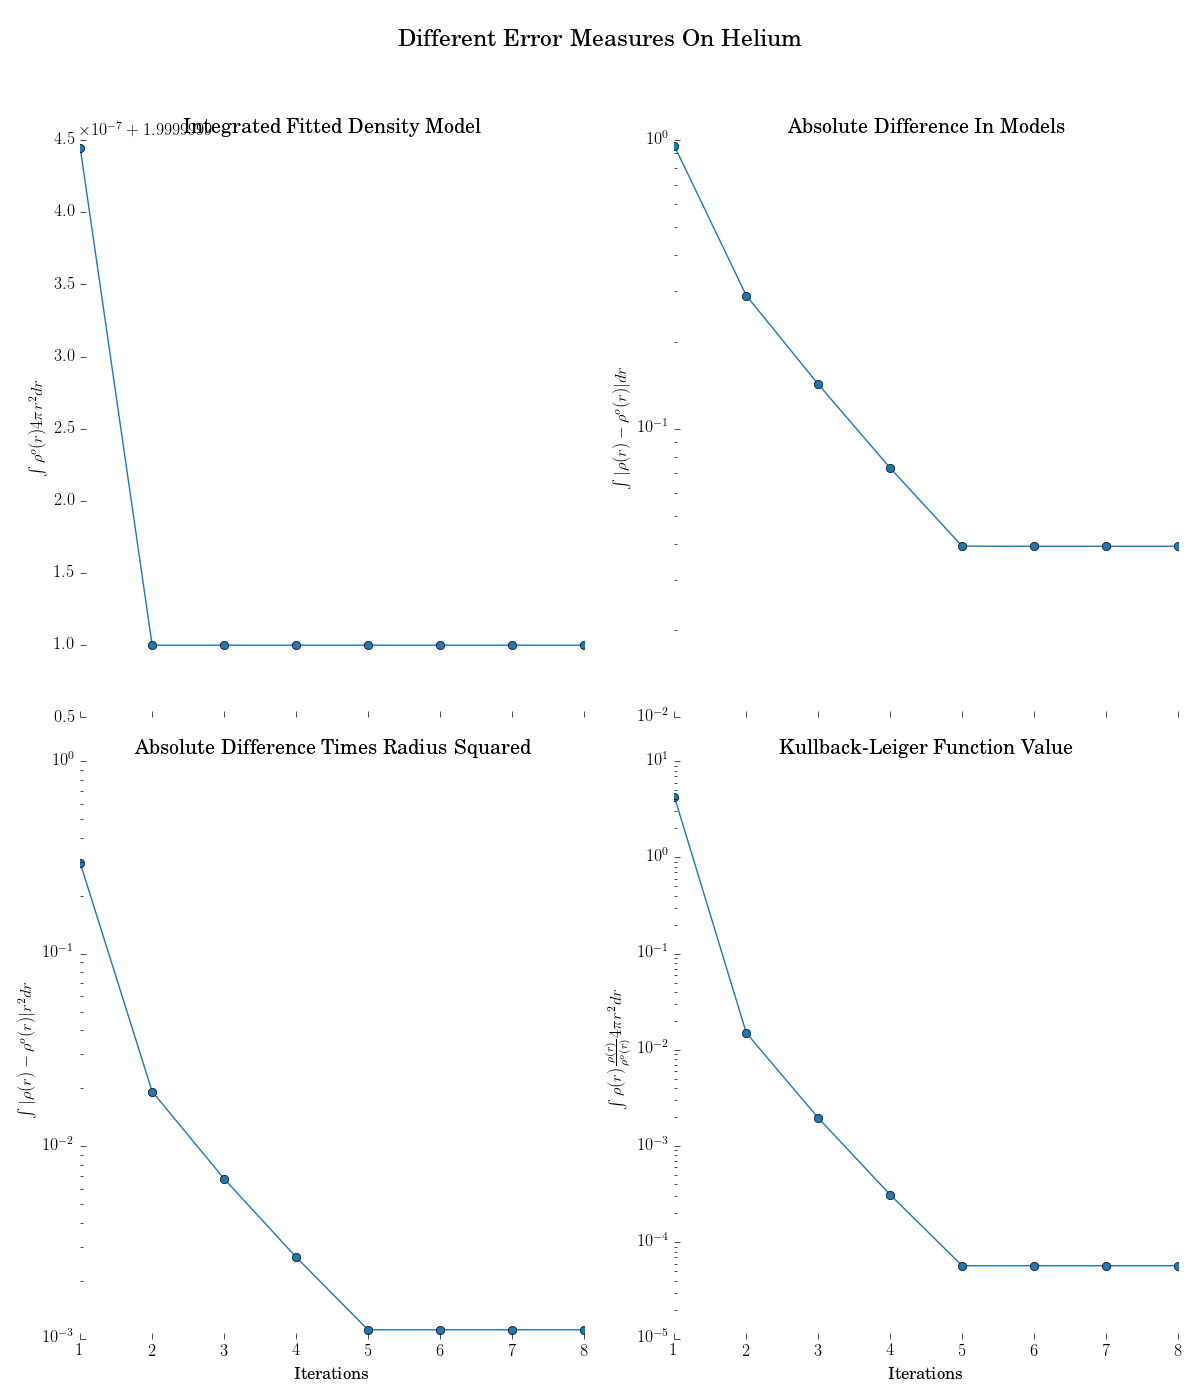
\includegraphics[scale=0.32]{results/he/error_plot_using_greedy-mbis.png}}
\fbox{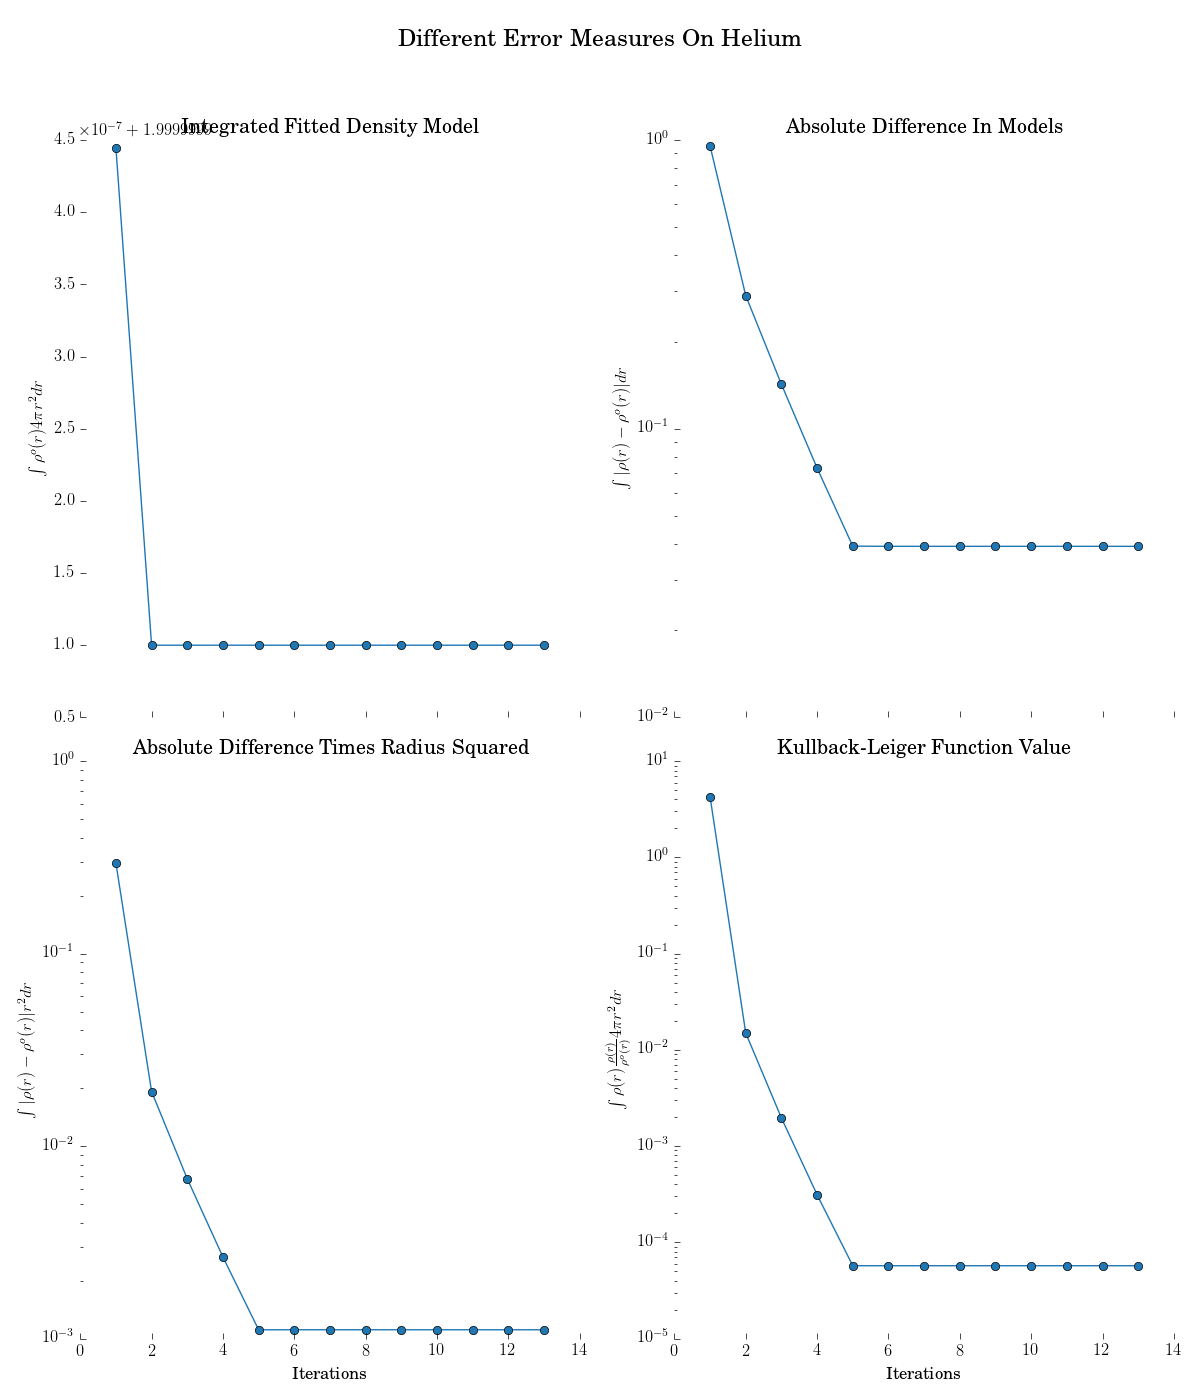
\includegraphics[scale=0.32]{results_original/he/error_plot_using_greedy-mbis.png}}
\fbox{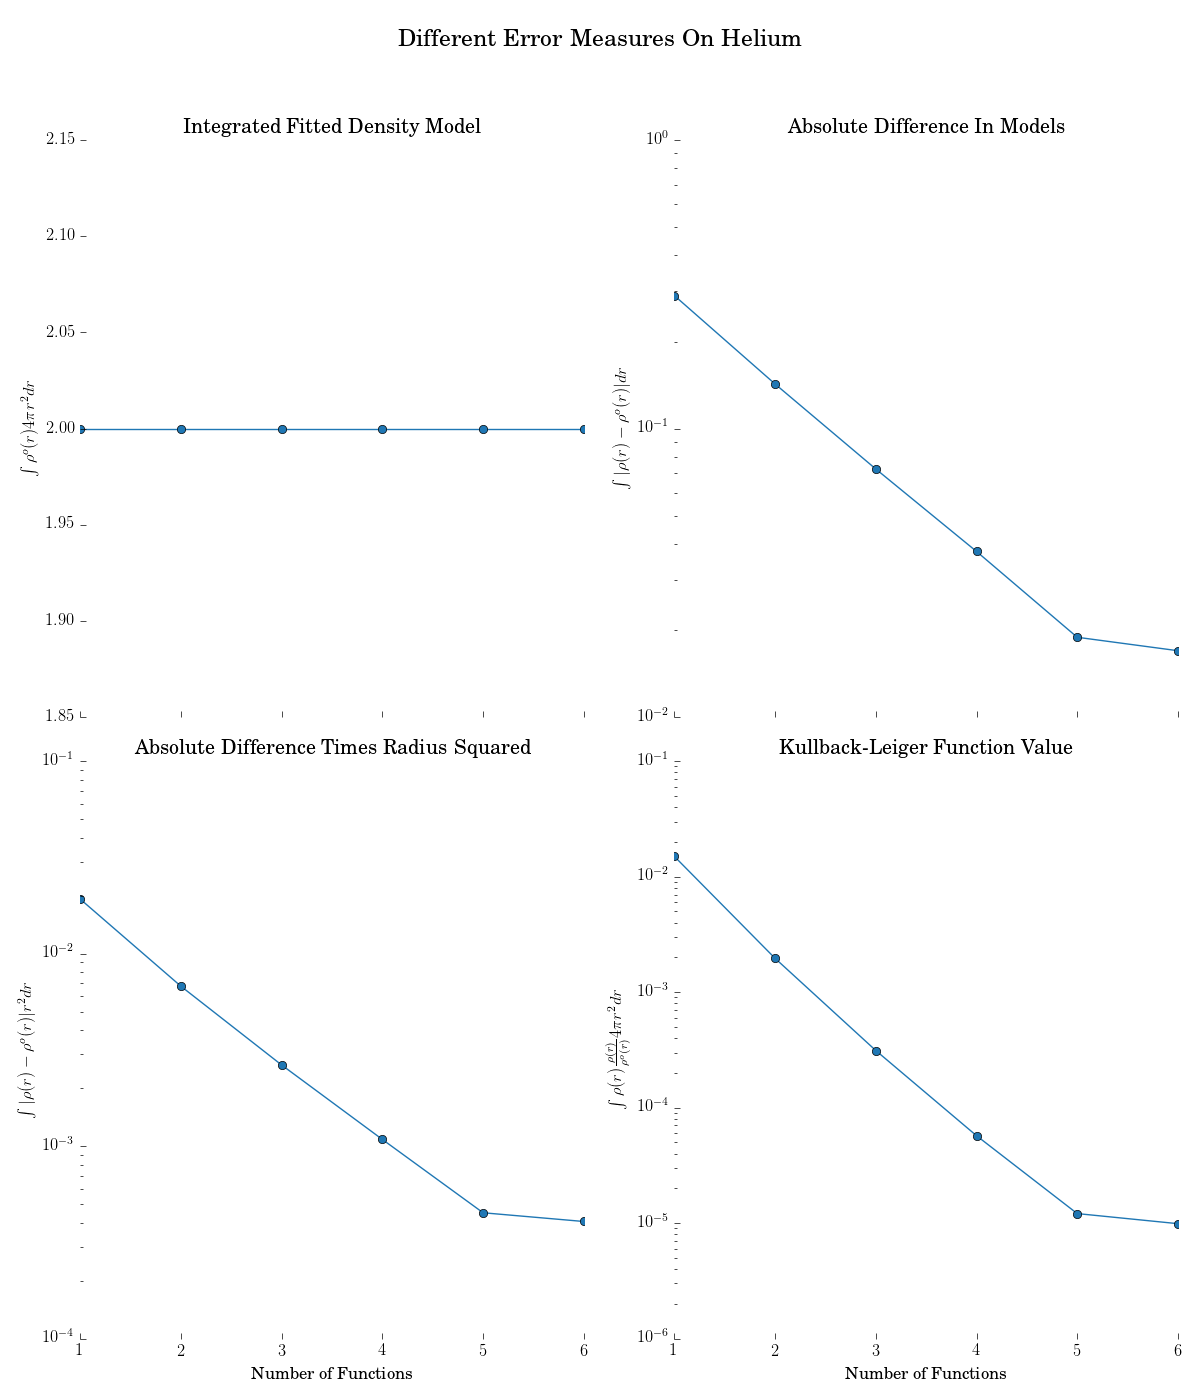
\includegraphics[scale=0.32]{results_redudancies/he/error_plot_using_greedy-mbis.png}} 

\subsection{Li}
\fbox{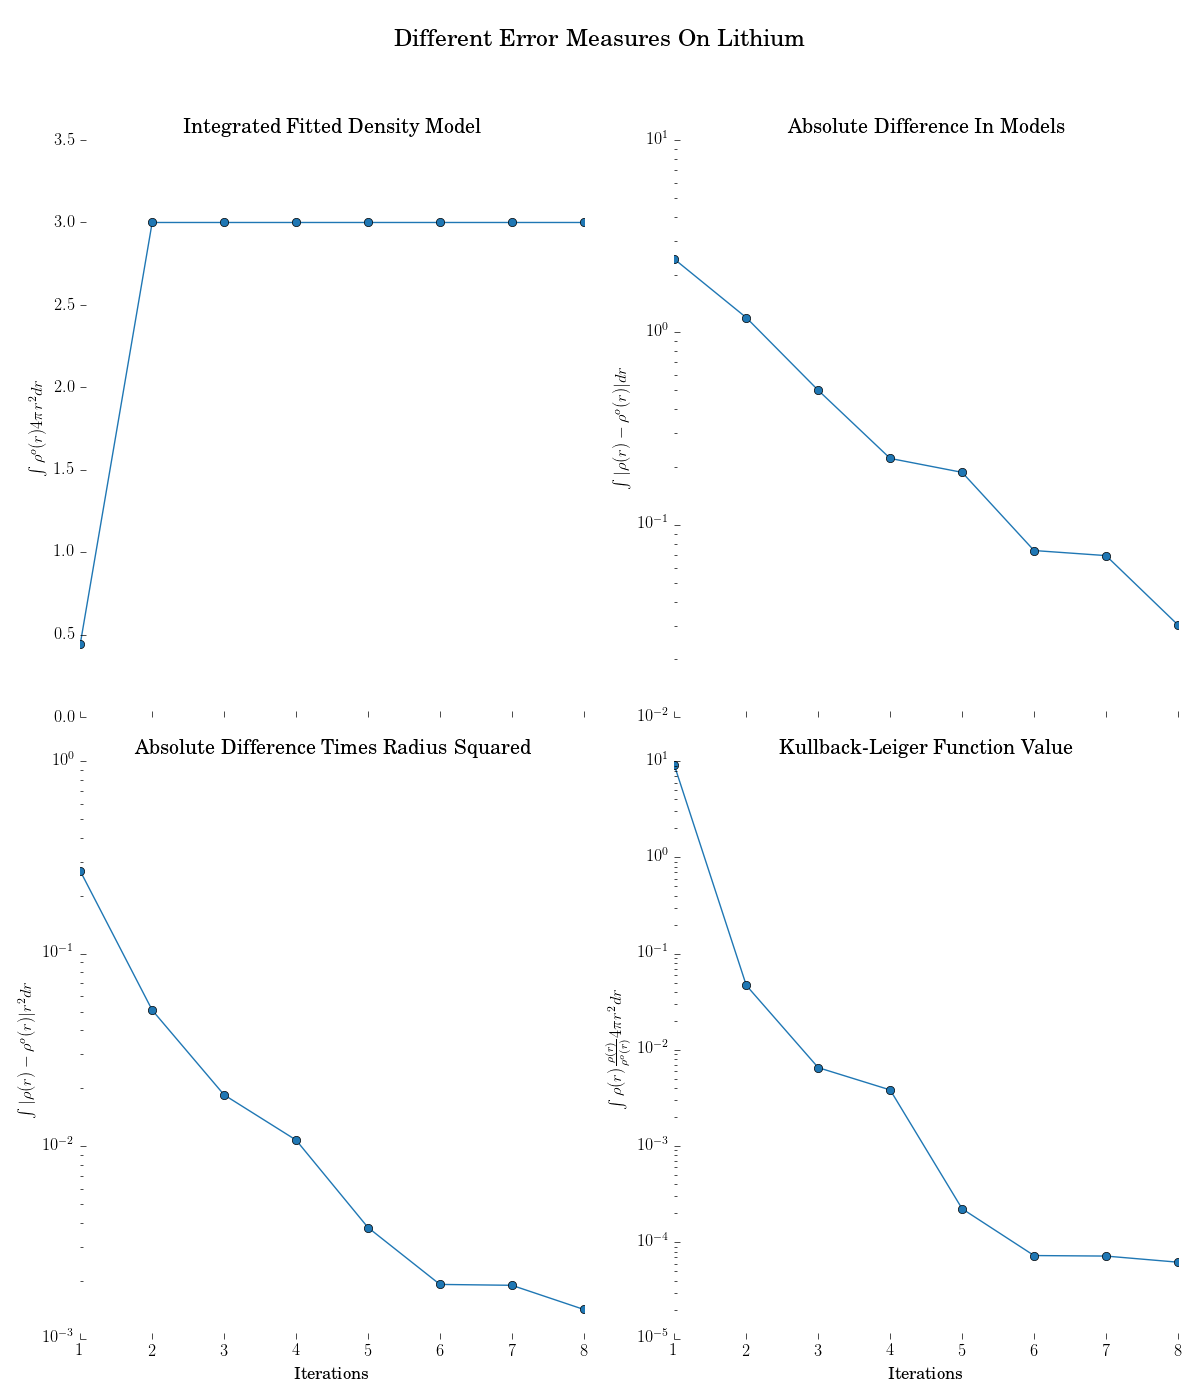
\includegraphics[scale=0.32]{results/li/error_plot_using_greedy-mbis.png}}
\fbox{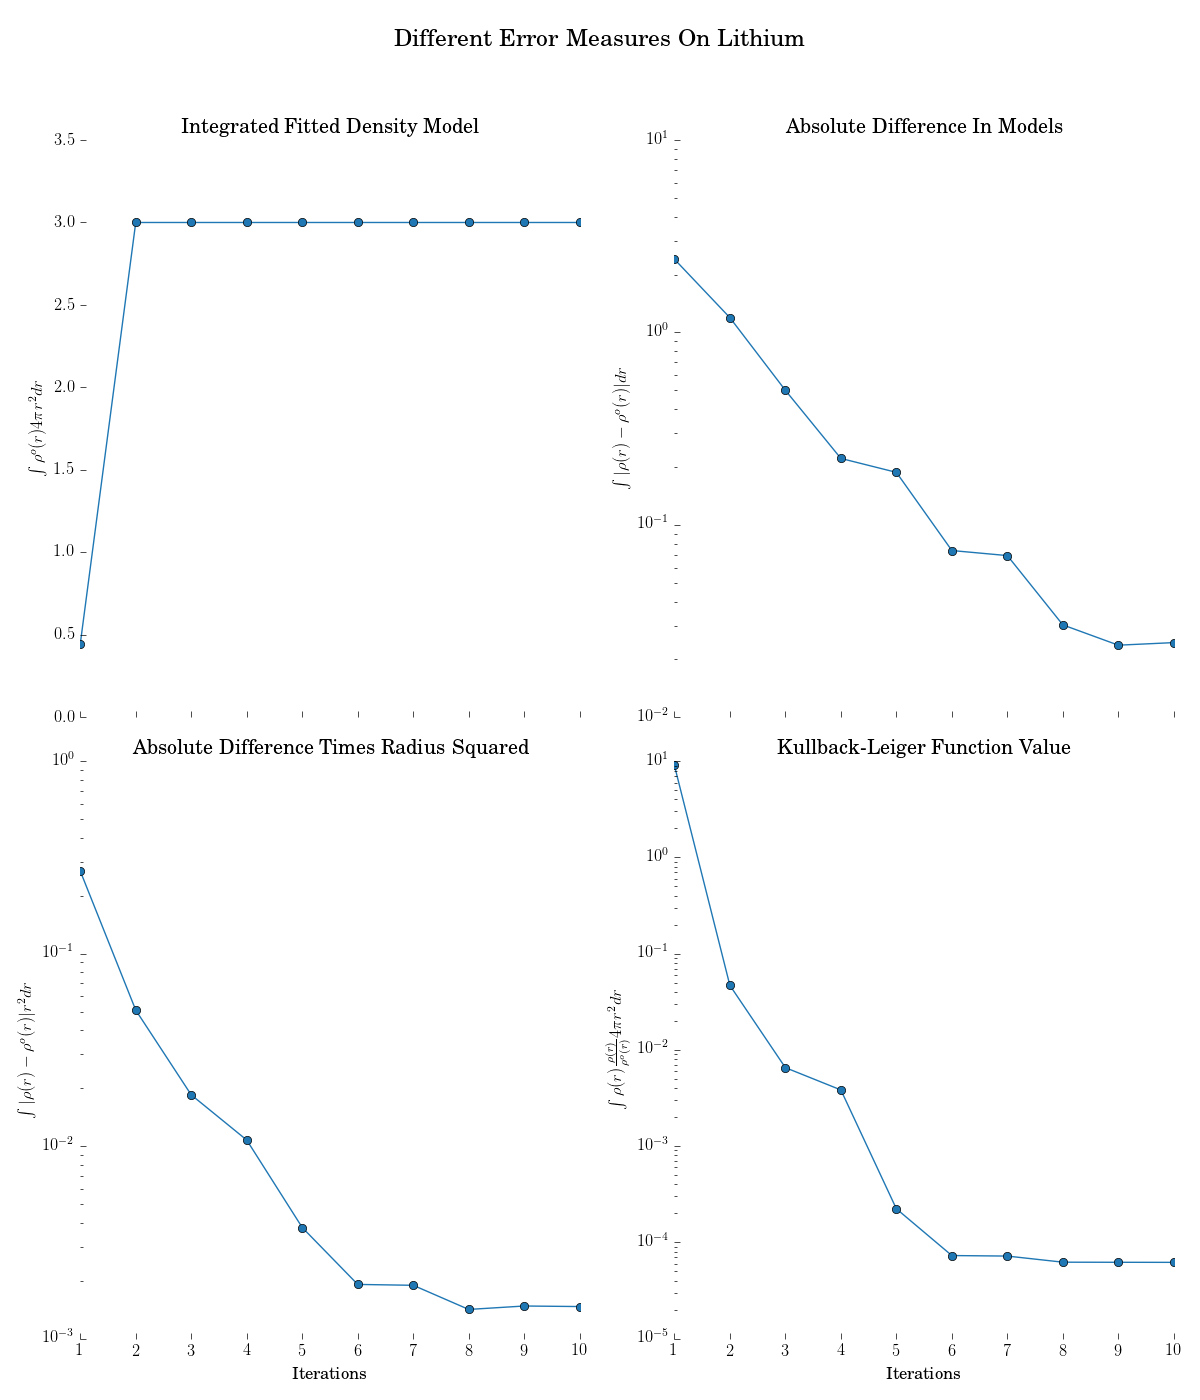
\includegraphics[scale=0.32]{results_original/li/error_plot_using_greedy-mbis.png}}
\fbox{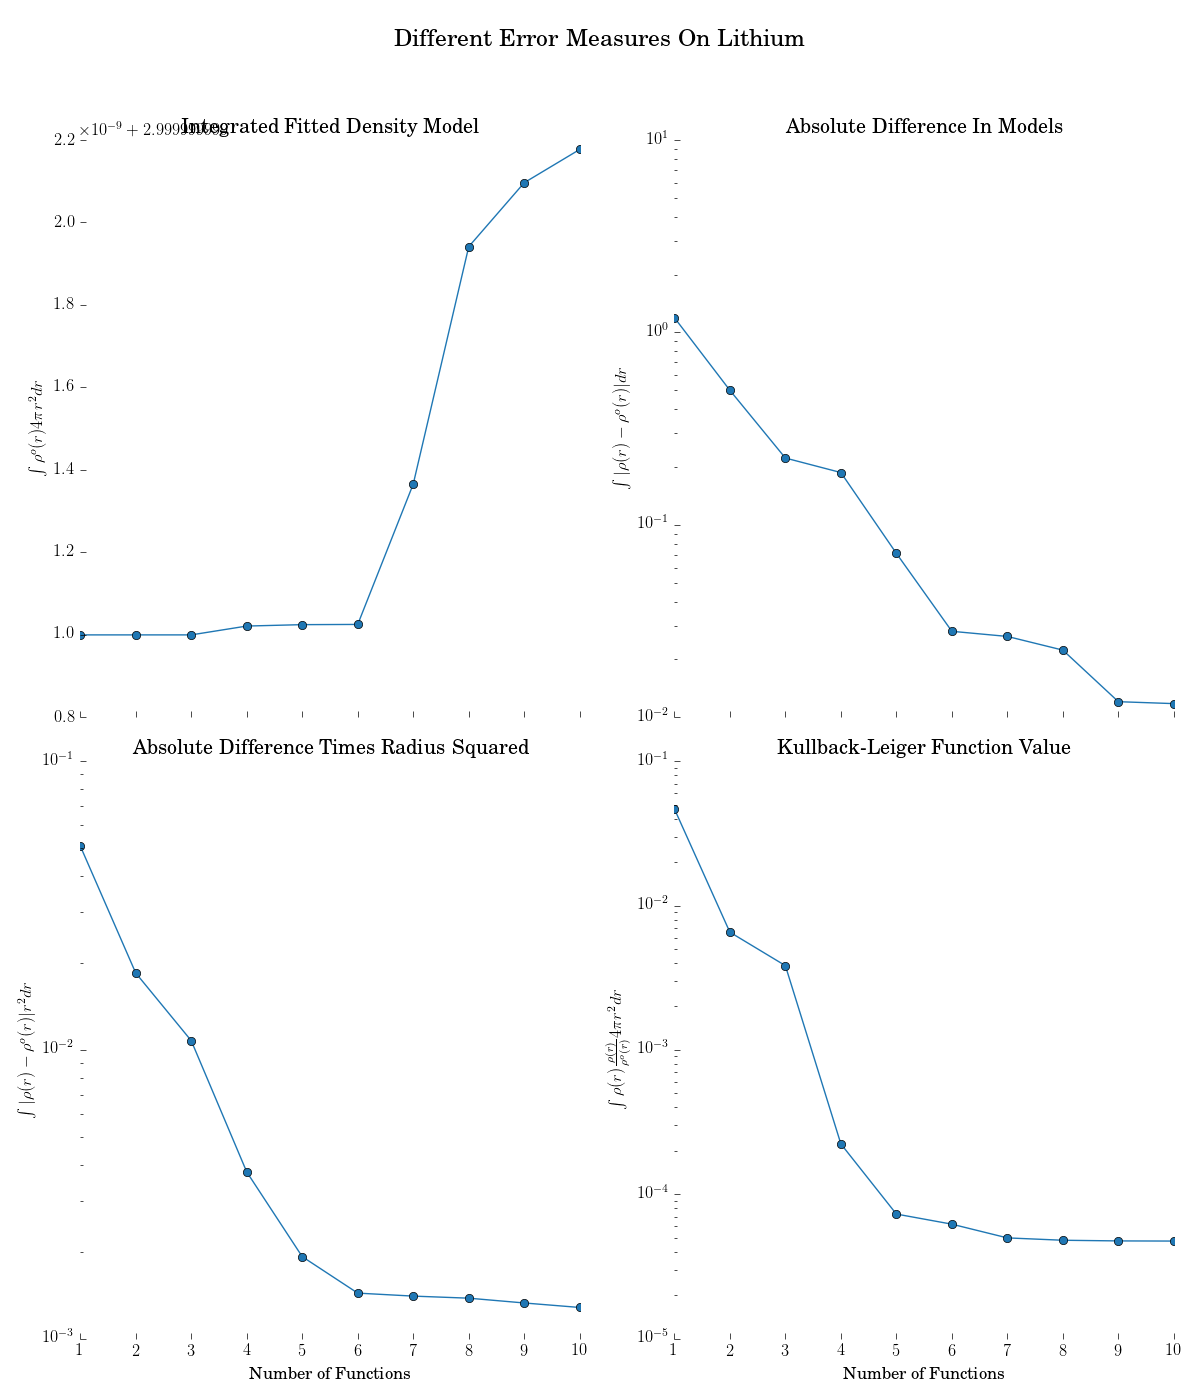
\includegraphics[scale=0.32]{results_redudancies/li/error_plot_using_greedy-mbis.png}}
\subsection{Be}
\fbox{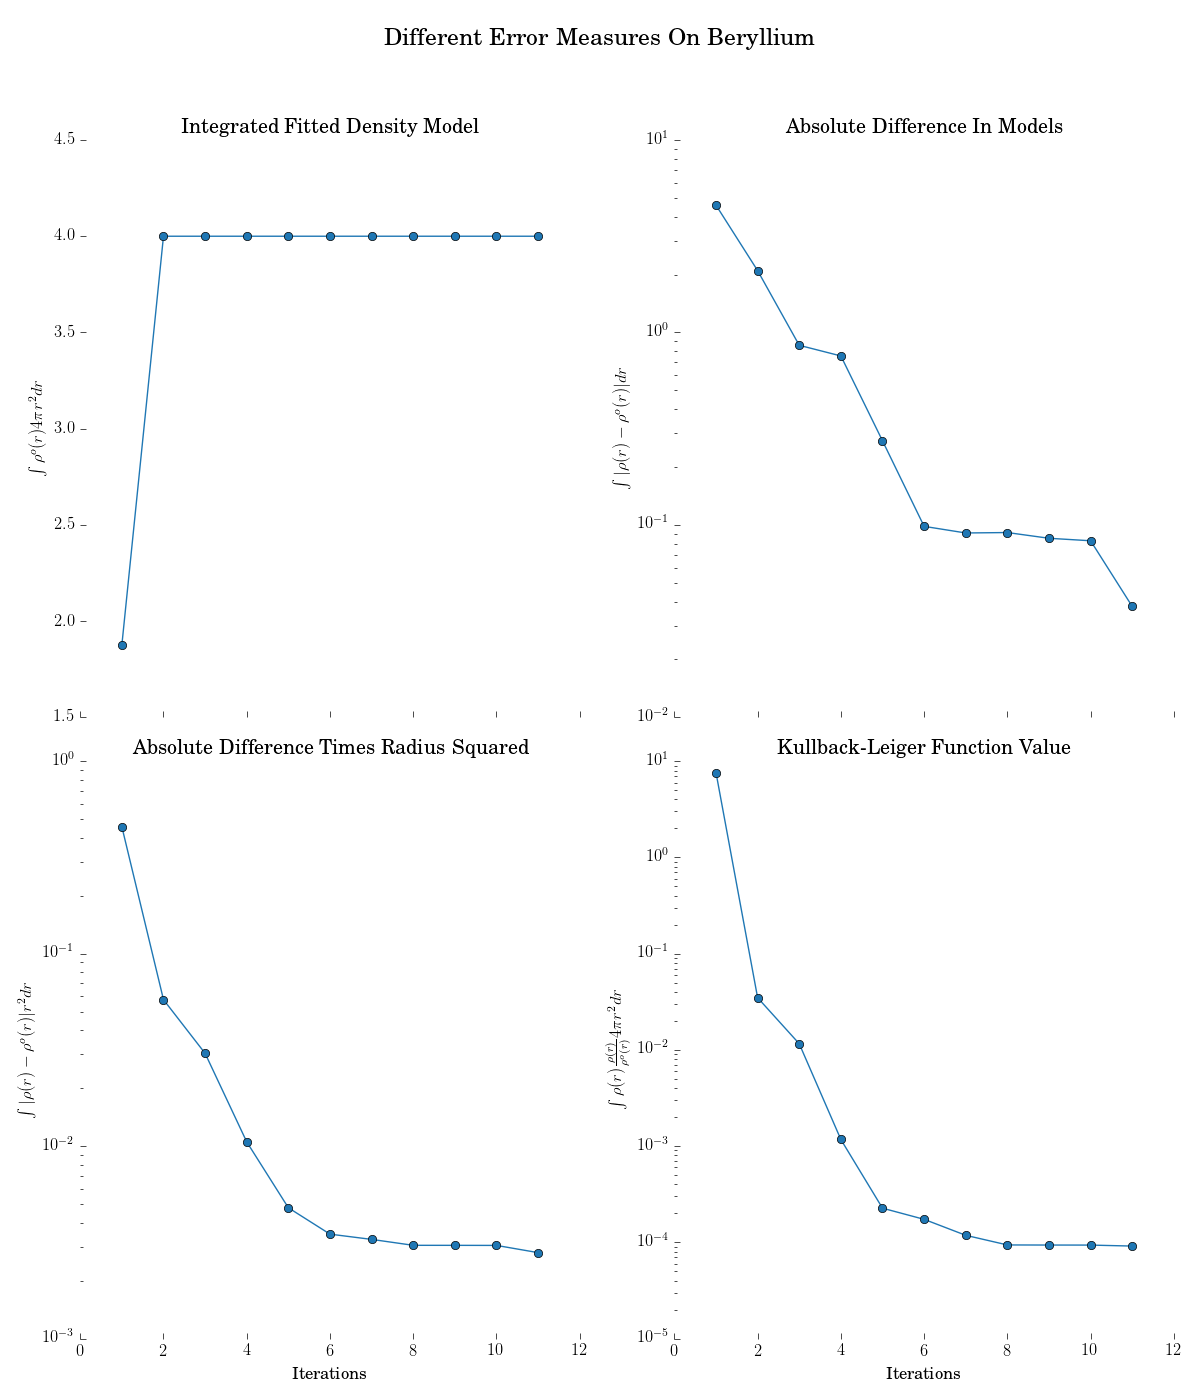
\includegraphics[scale=0.32]{results/be/error_plot_using_greedy-mbis.png}}
\fbox{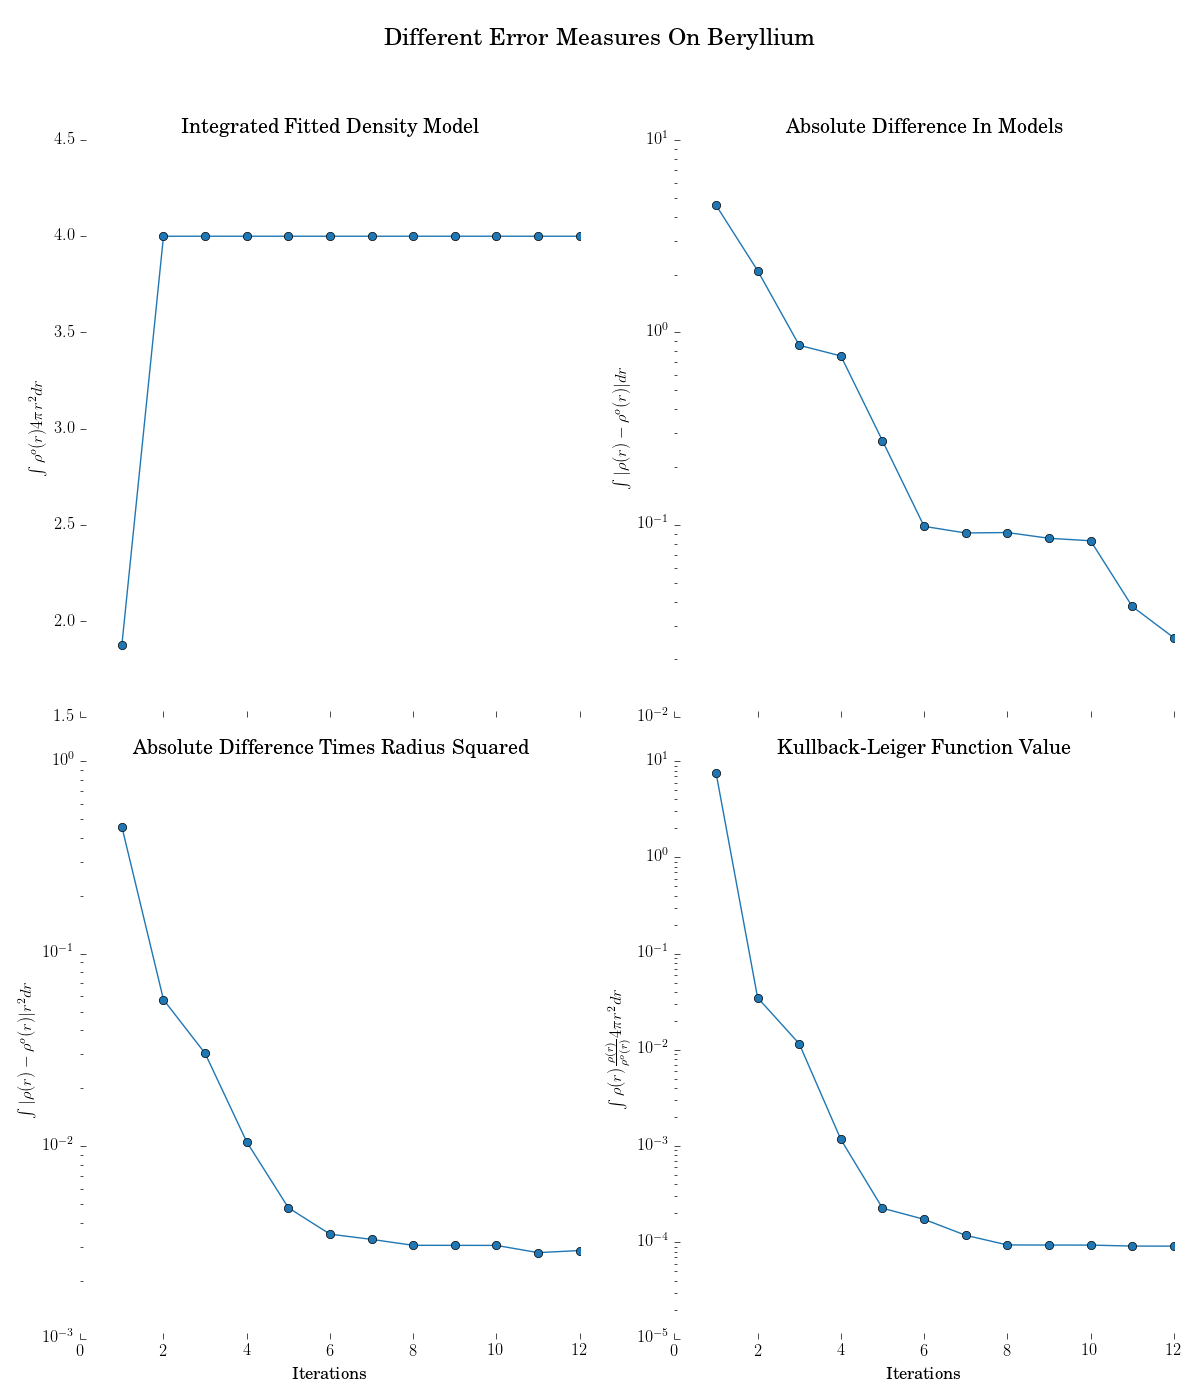
\includegraphics[scale=0.32]{results_original/be/error_plot_using_greedy-mbis.png}}
\fbox{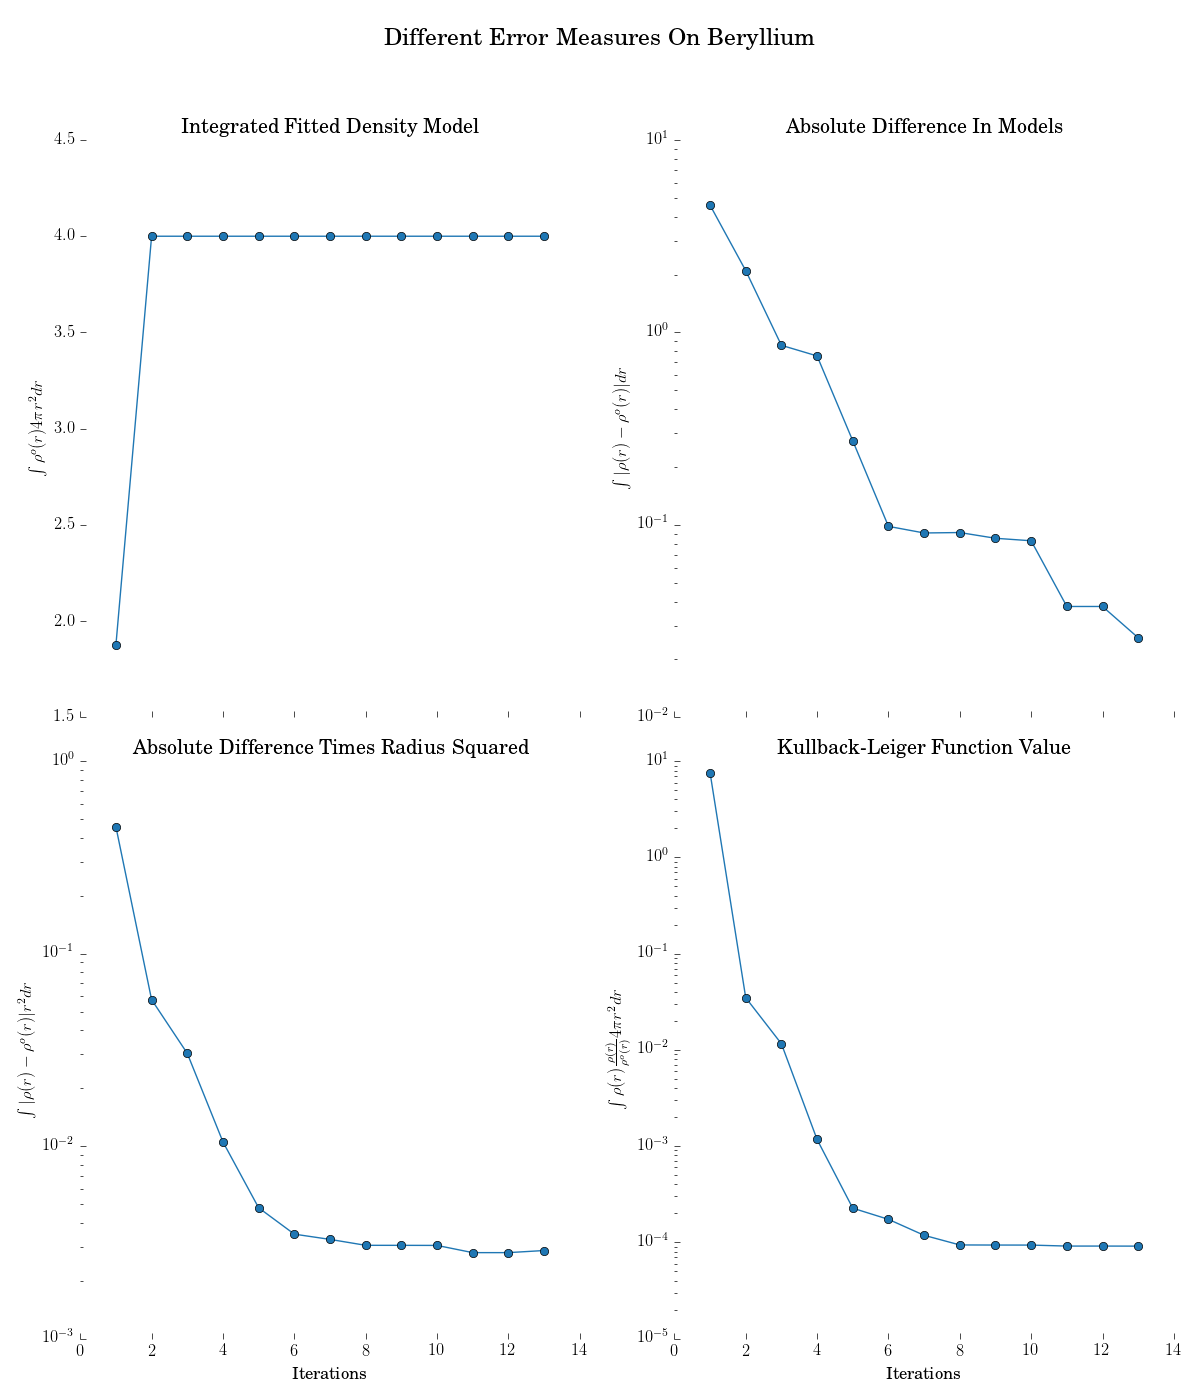
\includegraphics[scale=0.32]{results_redudancies/be/error_plot_using_greedy-mbis.png}}
\subsection{b}
\fbox{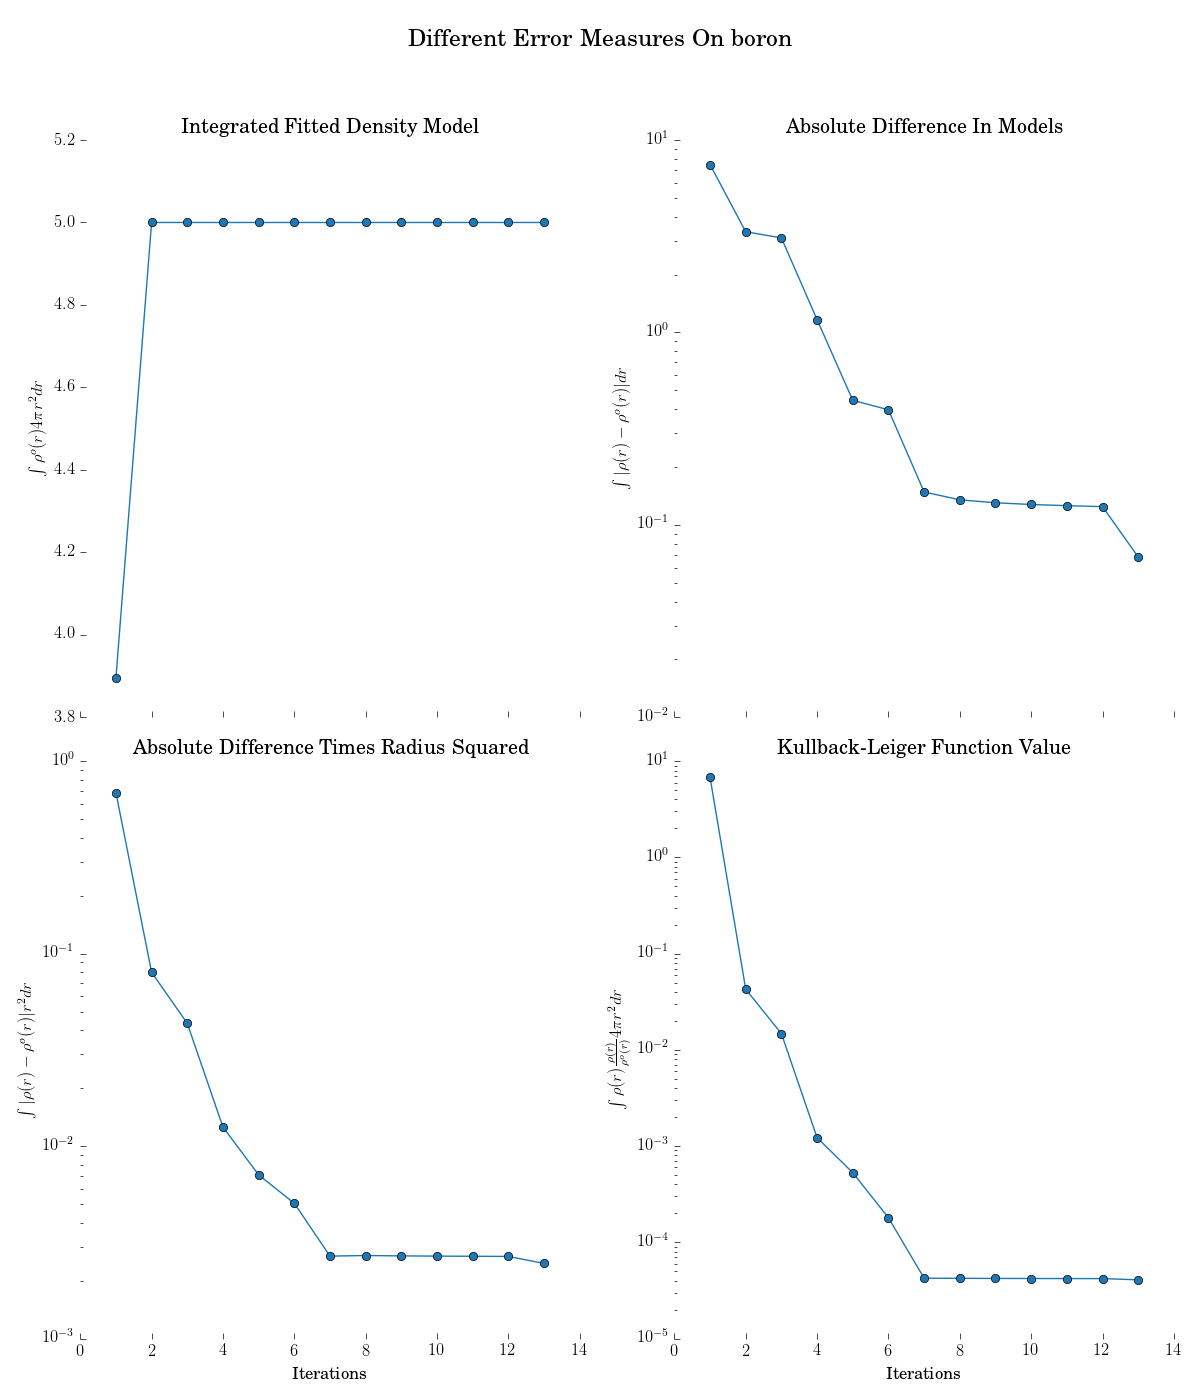
\includegraphics[scale=0.32]{results/b/error_plot_using_greedy-mbis.png}}
\fbox{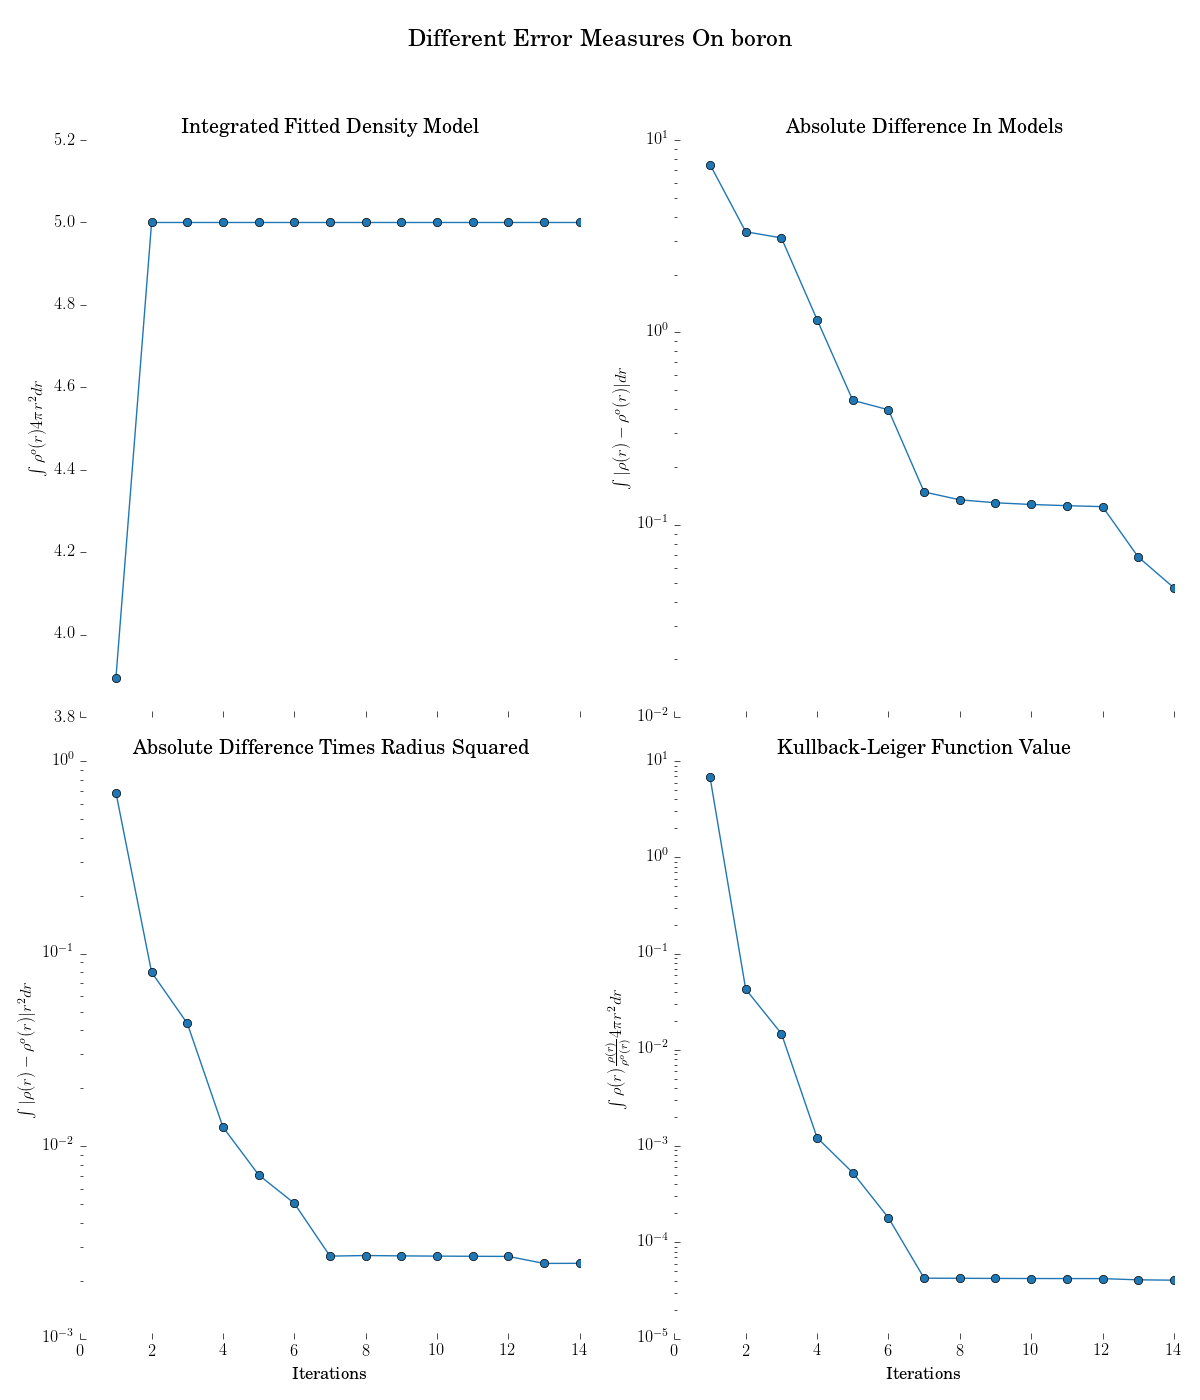
\includegraphics[scale=0.32]{results_original/b/error_plot_using_greedy-mbis.png}}
\fbox{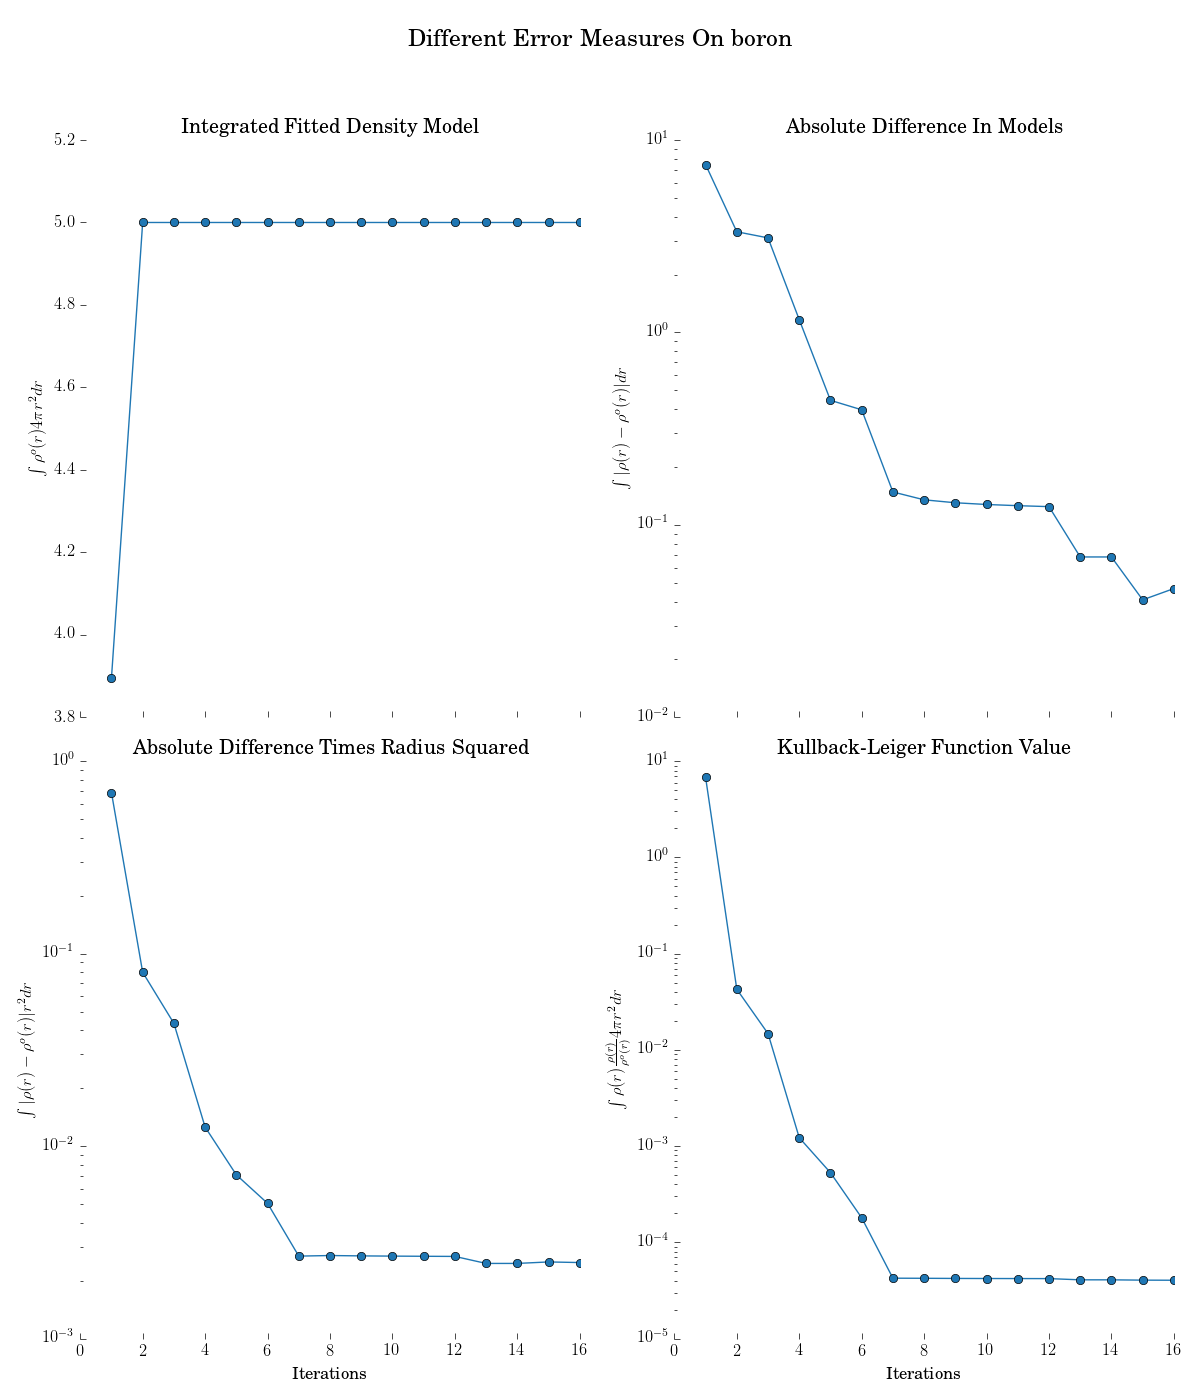
\includegraphics[scale=0.32]{results_redudancies/b/error_plot_using_greedy-mbis.png}}
\subsection{c}
\fbox{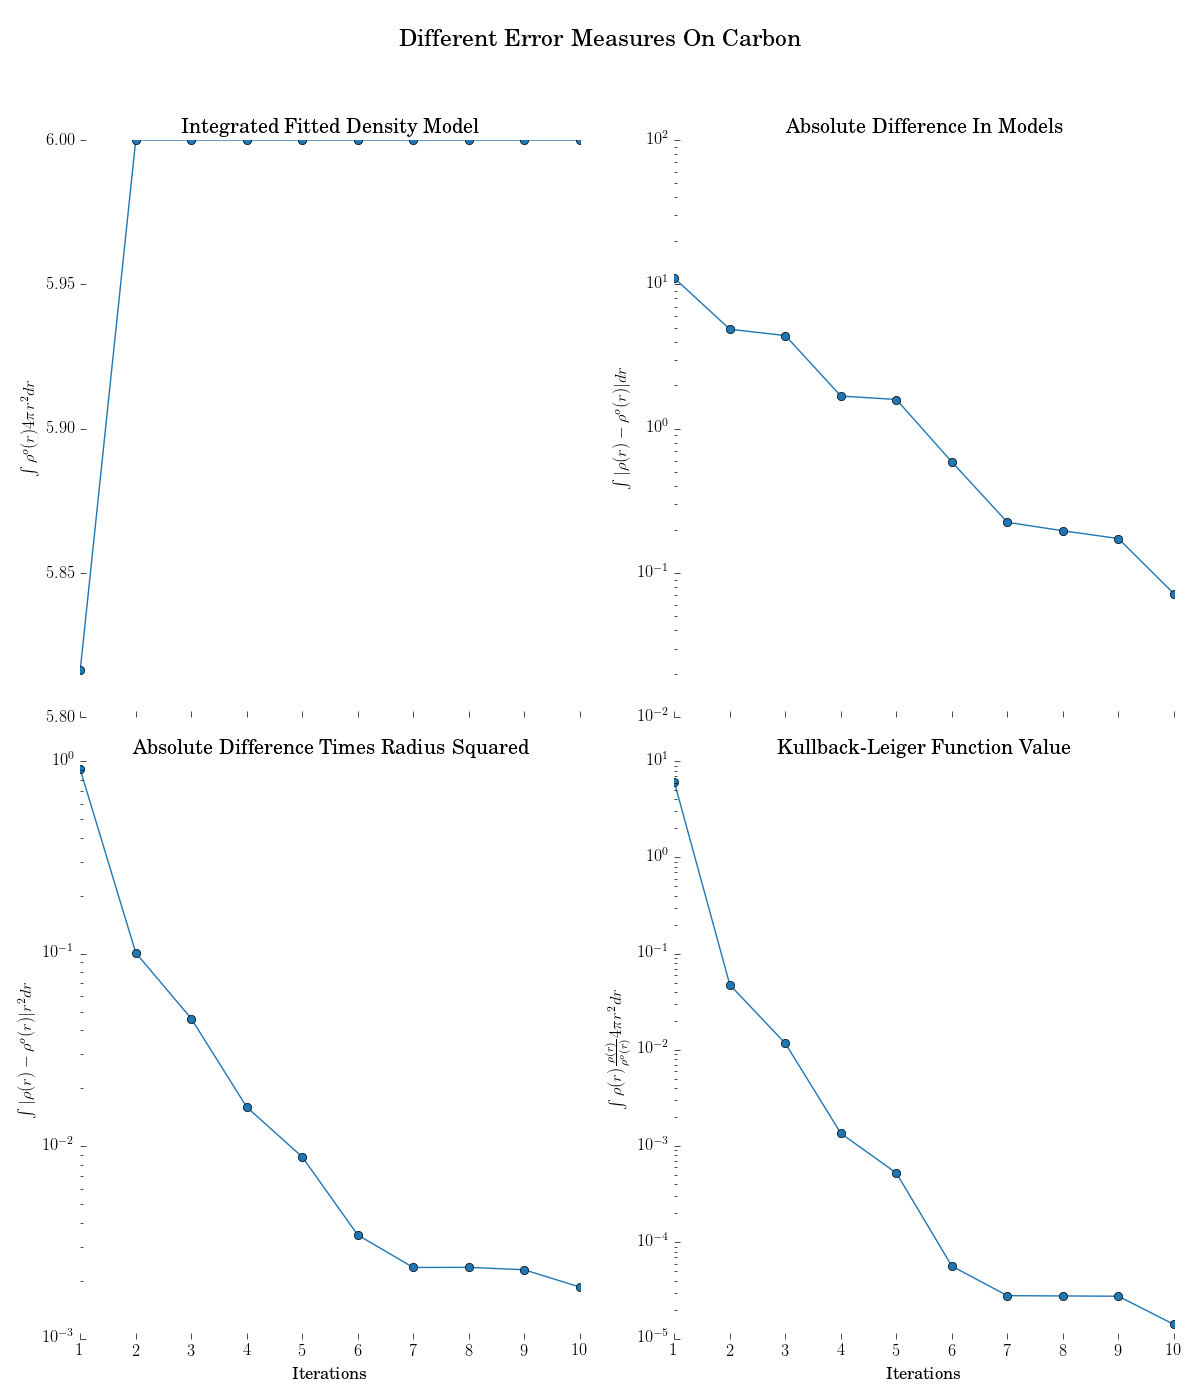
\includegraphics[scale=0.32]{results/c/error_plot_using_greedy-mbis.png}}
\fbox{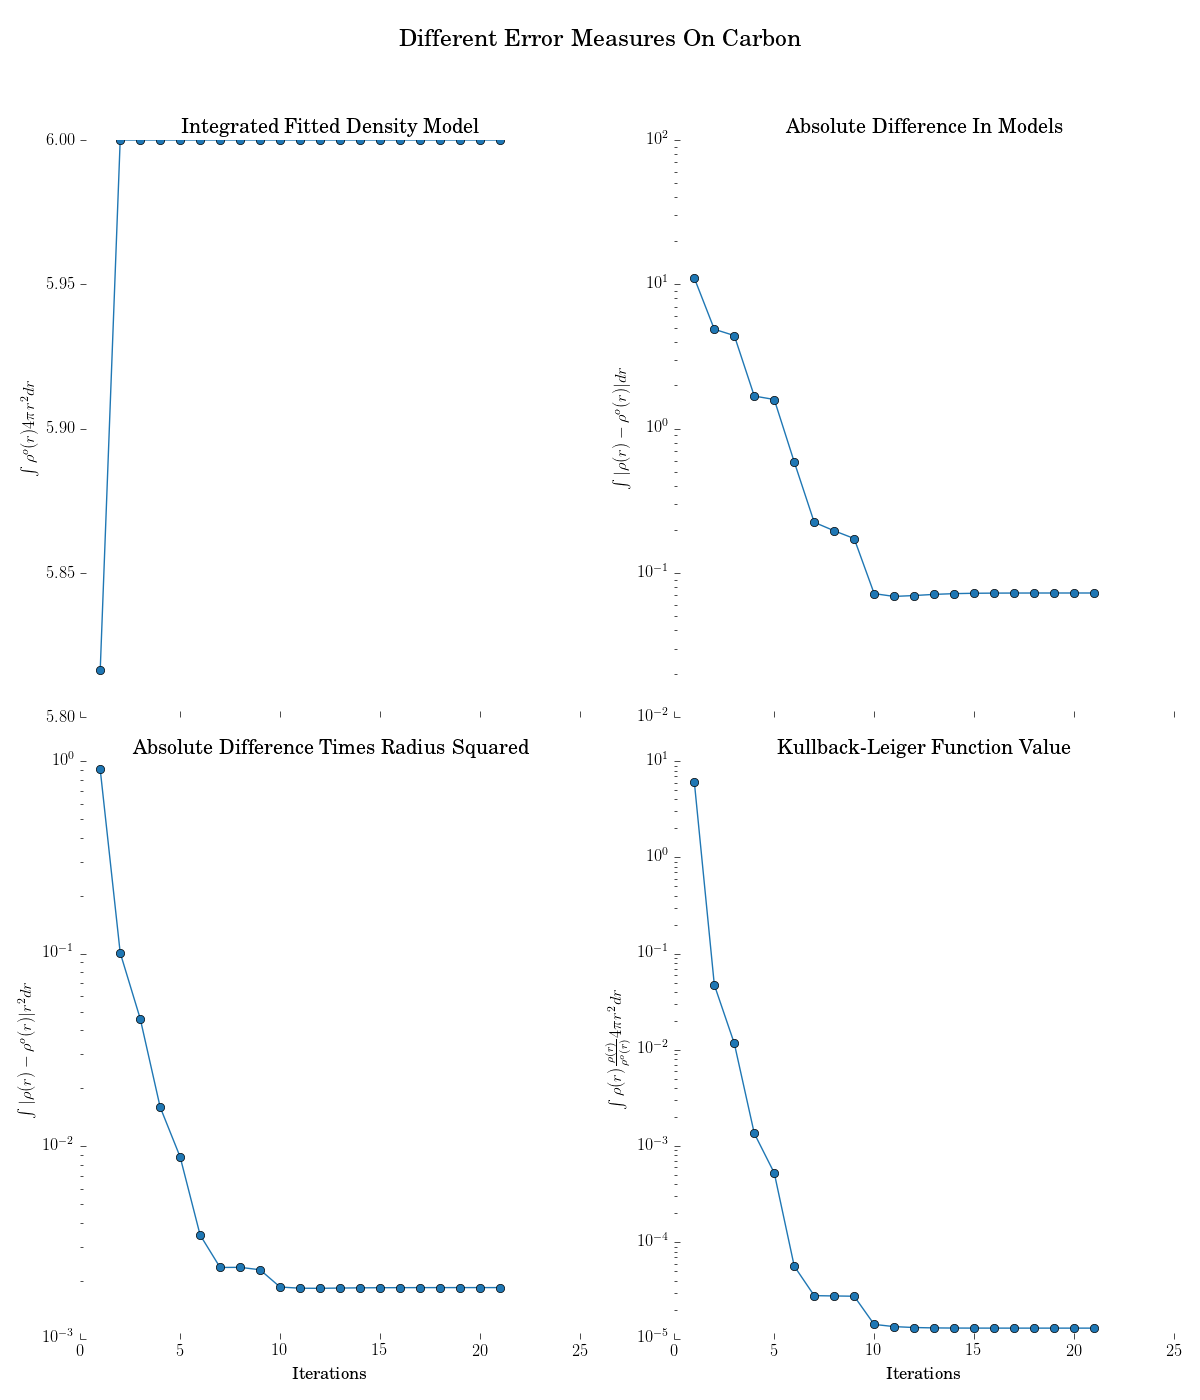
\includegraphics[scale=0.32]{results_original/c/error_plot_using_greedy-mbis.png}}
\fbox{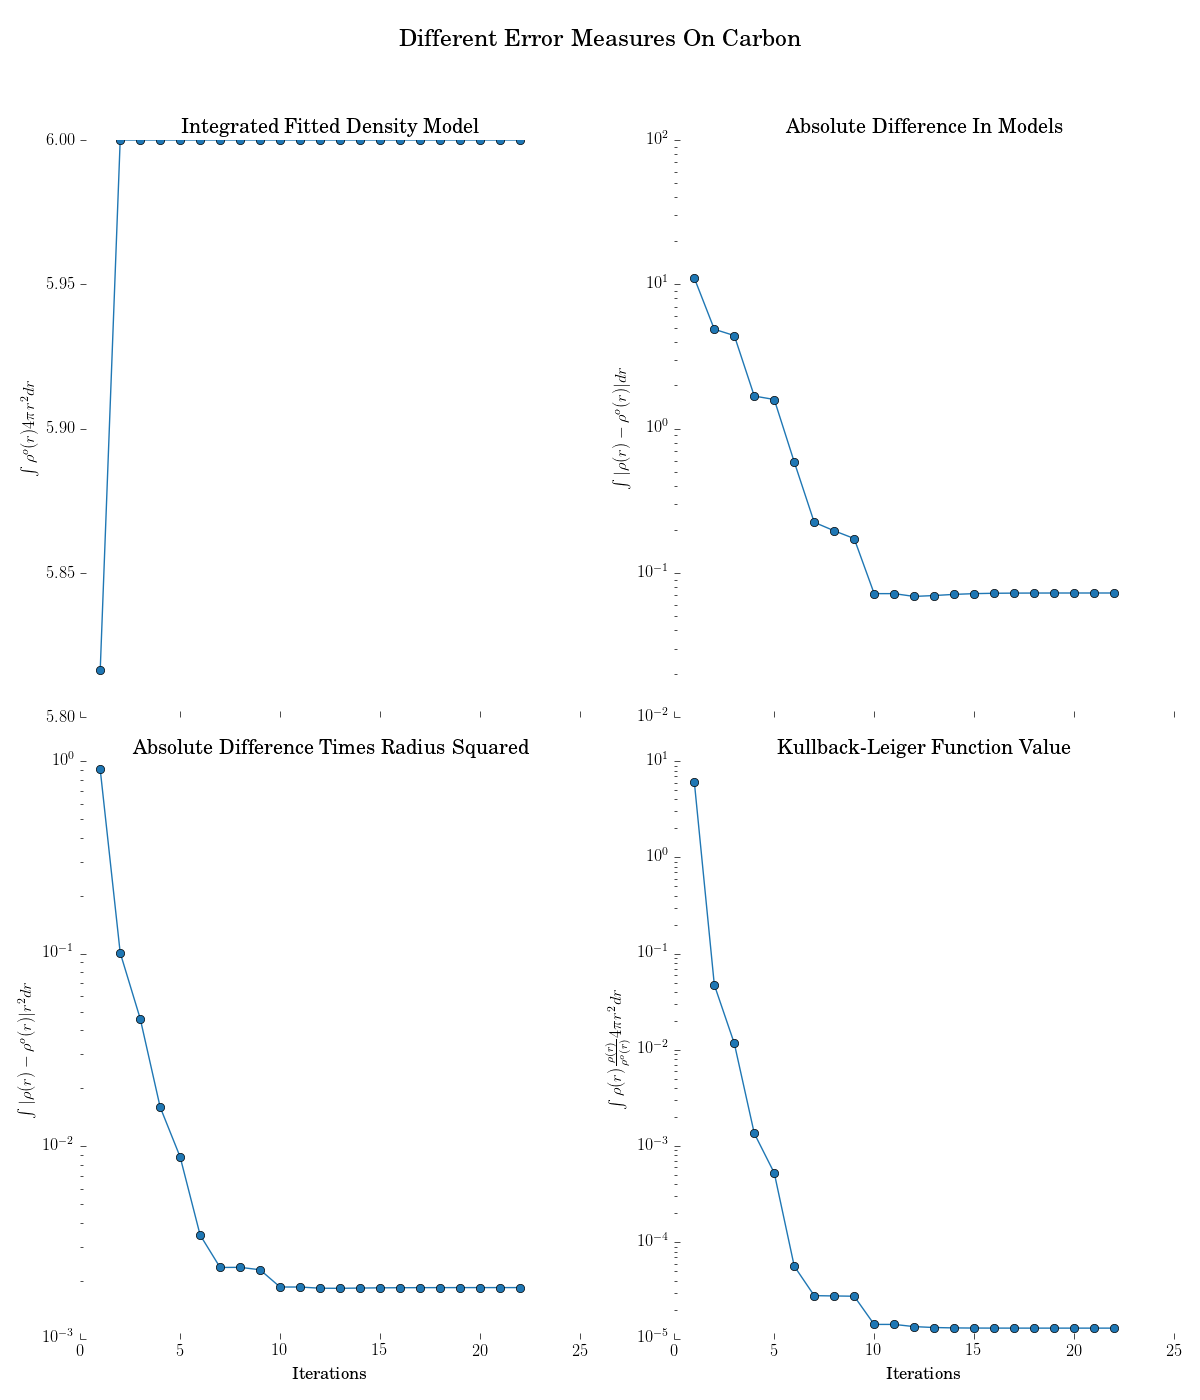
\includegraphics[scale=0.32]{results_redudancies/c/error_plot_using_greedy-mbis.png}}
\subsection{n}
\fbox{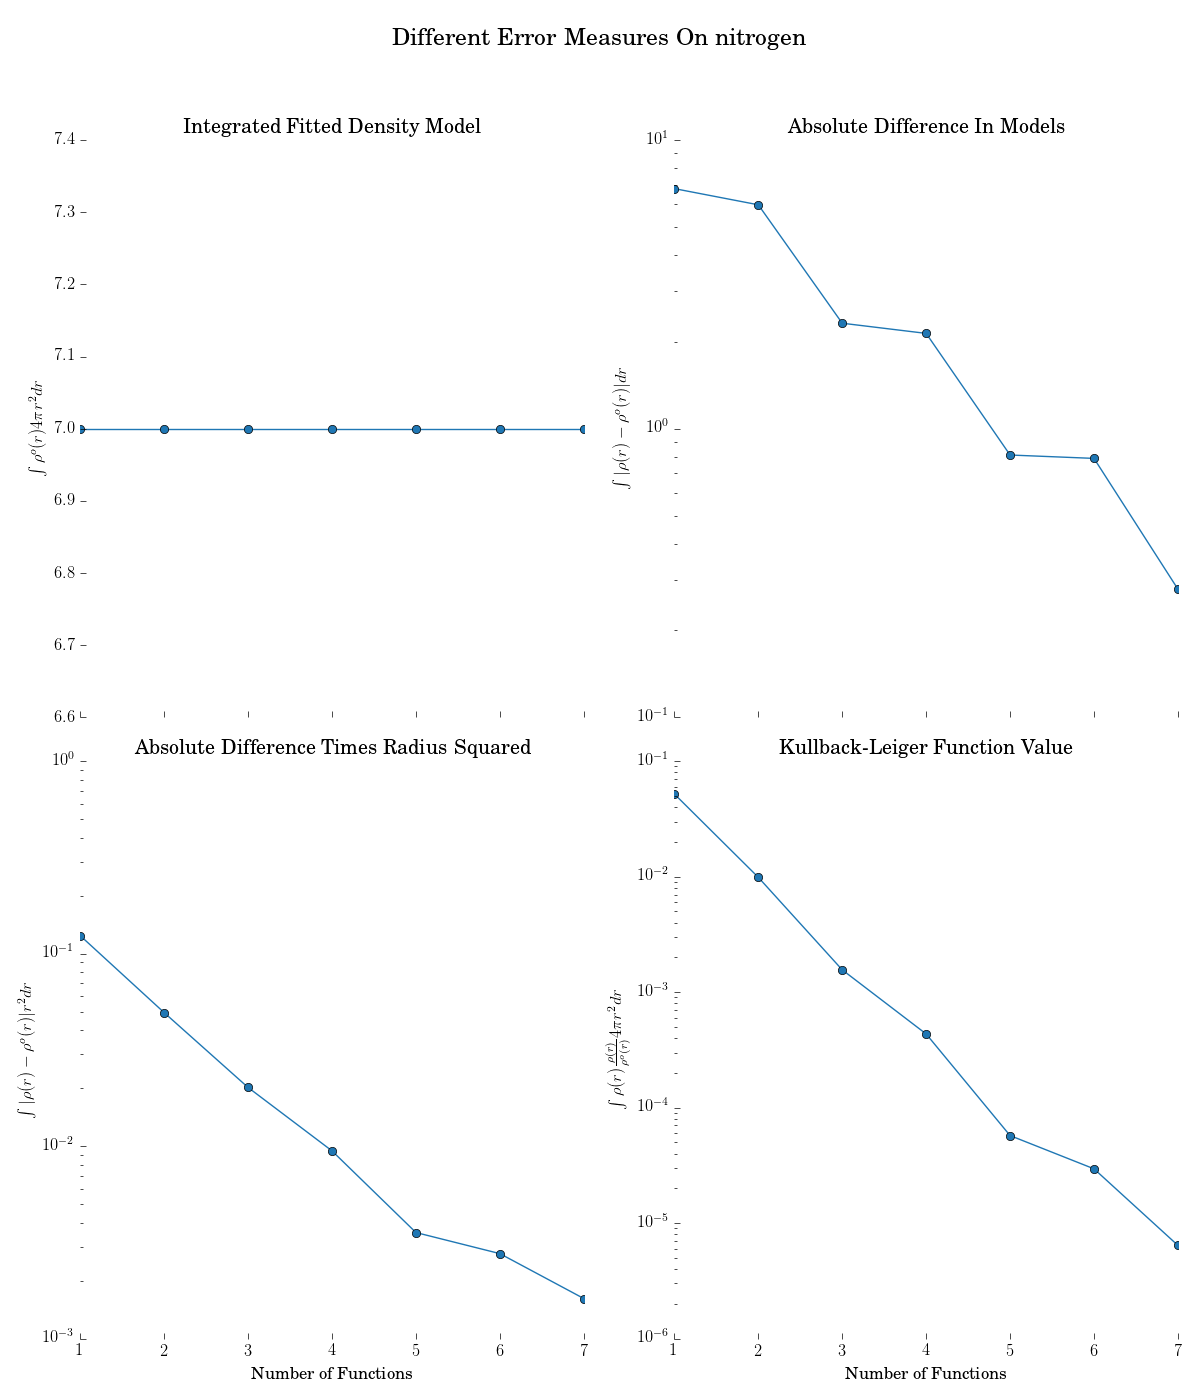
\includegraphics[scale=0.32]{results/n/error_plot_using_greedy-mbis.png}}
\fbox{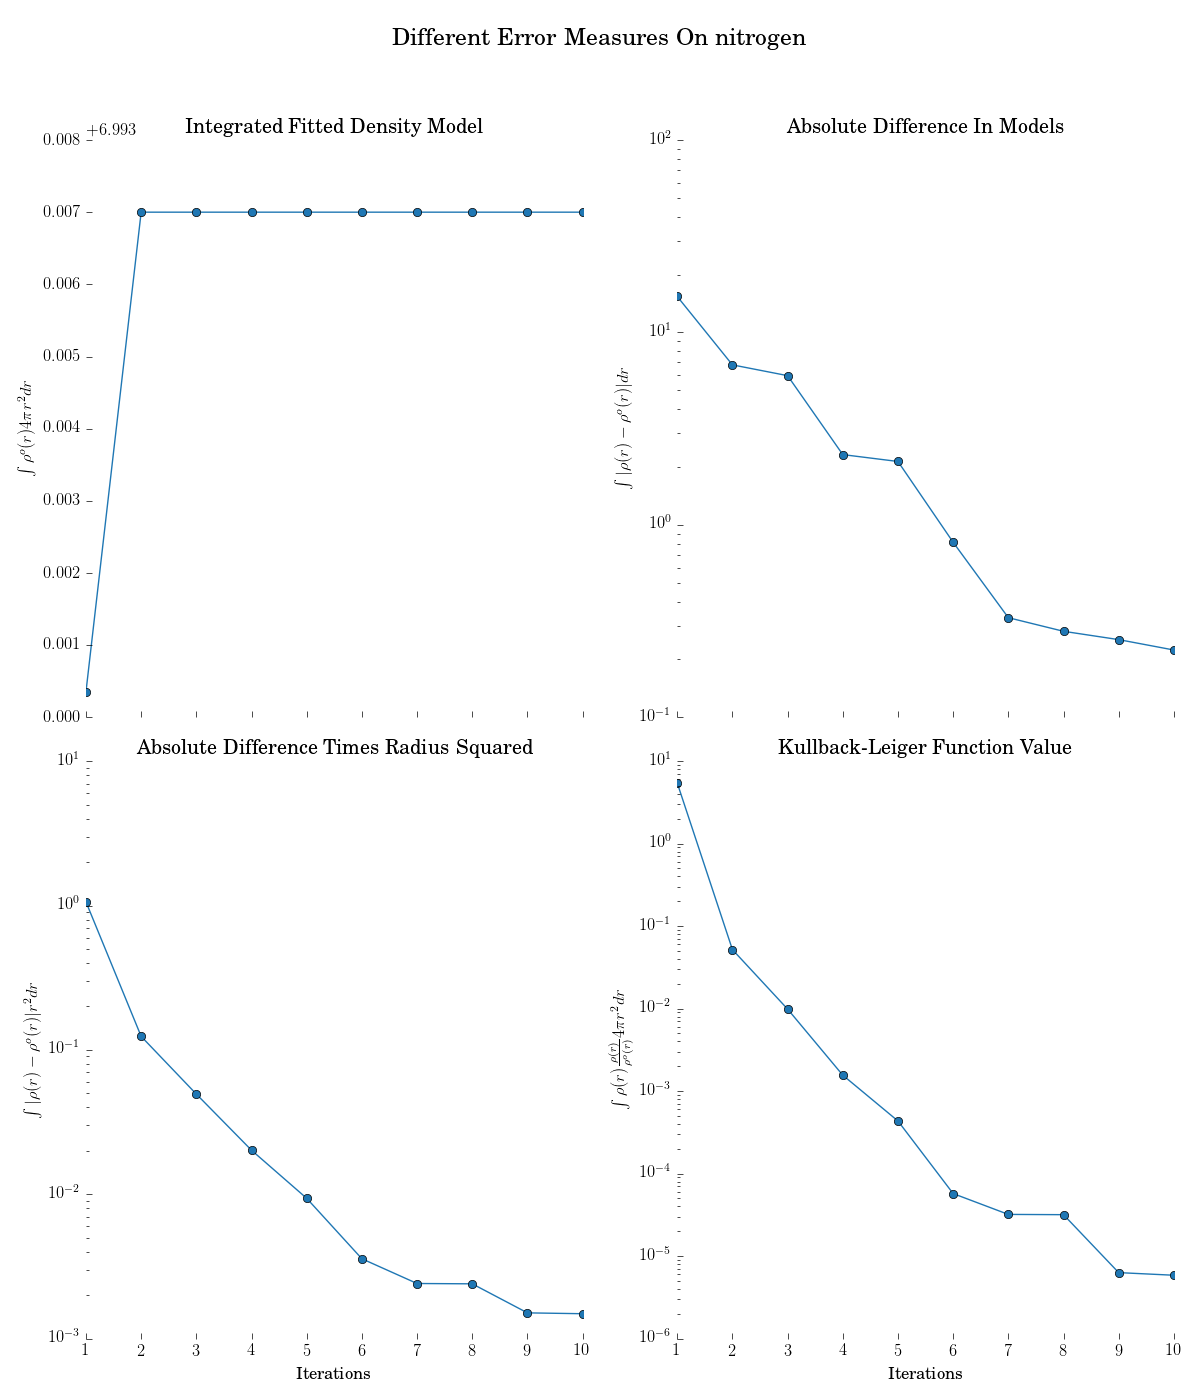
\includegraphics[scale=0.32]{results_original/n/error_plot_using_greedy-mbis.png}}
\fbox{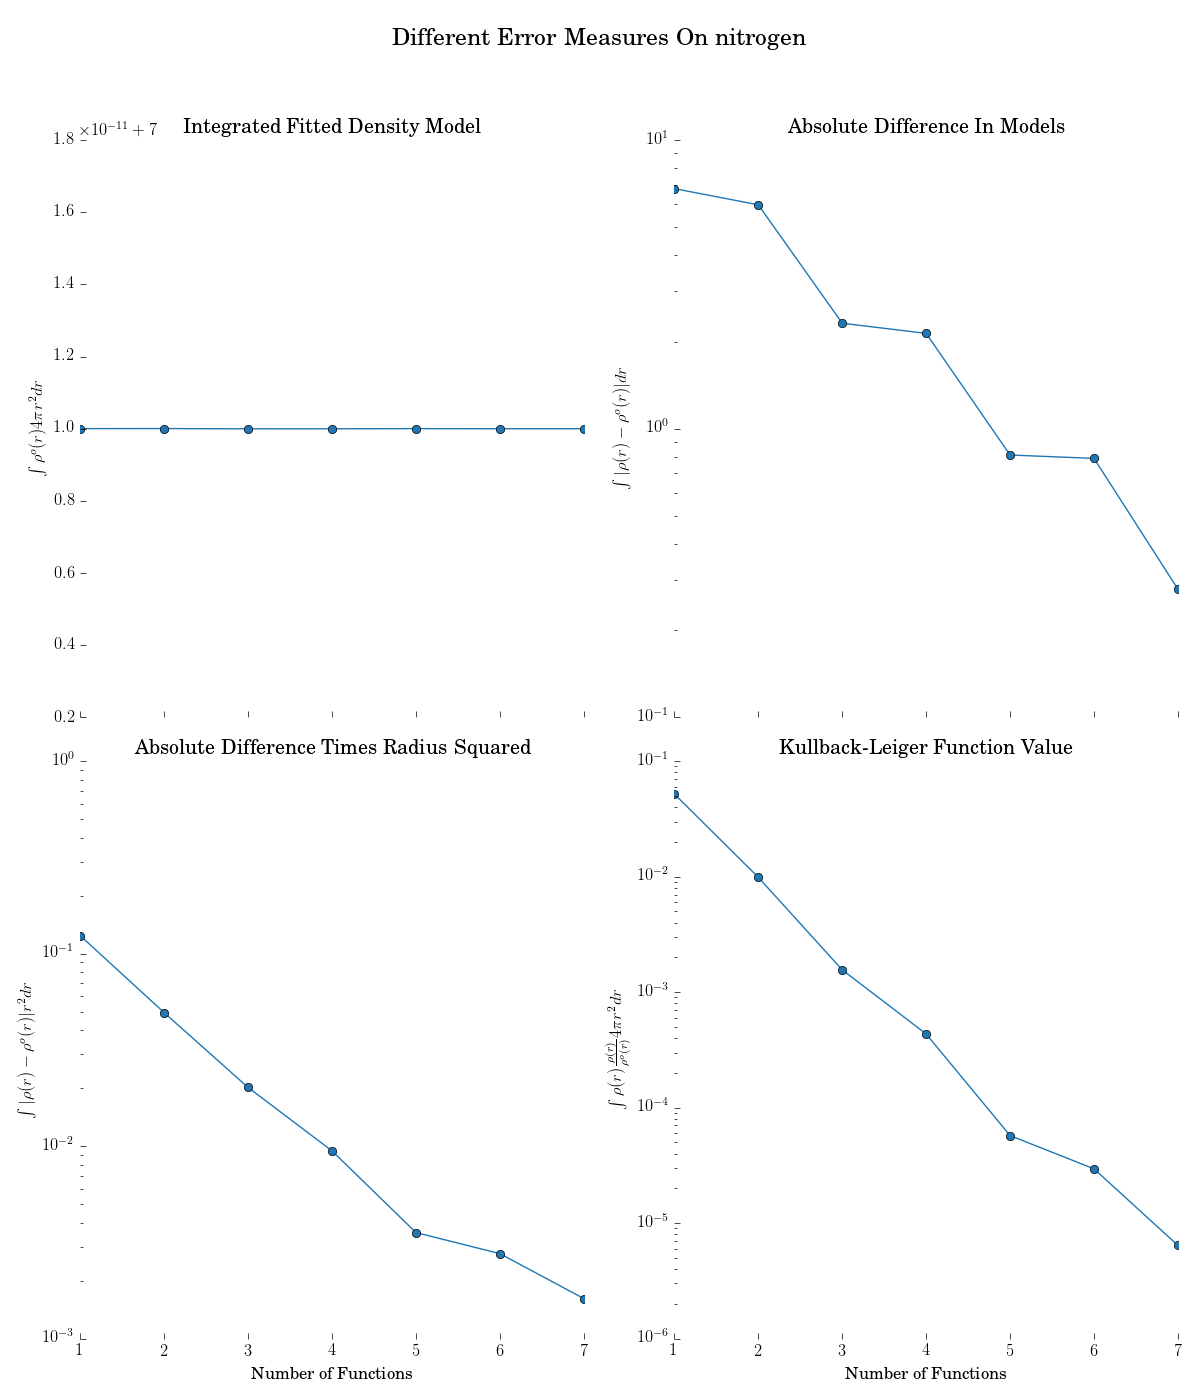
\includegraphics[scale=0.32]{results_redudancies/n/error_plot_using_greedy-mbis.png}}

\subsection{o}
\fbox{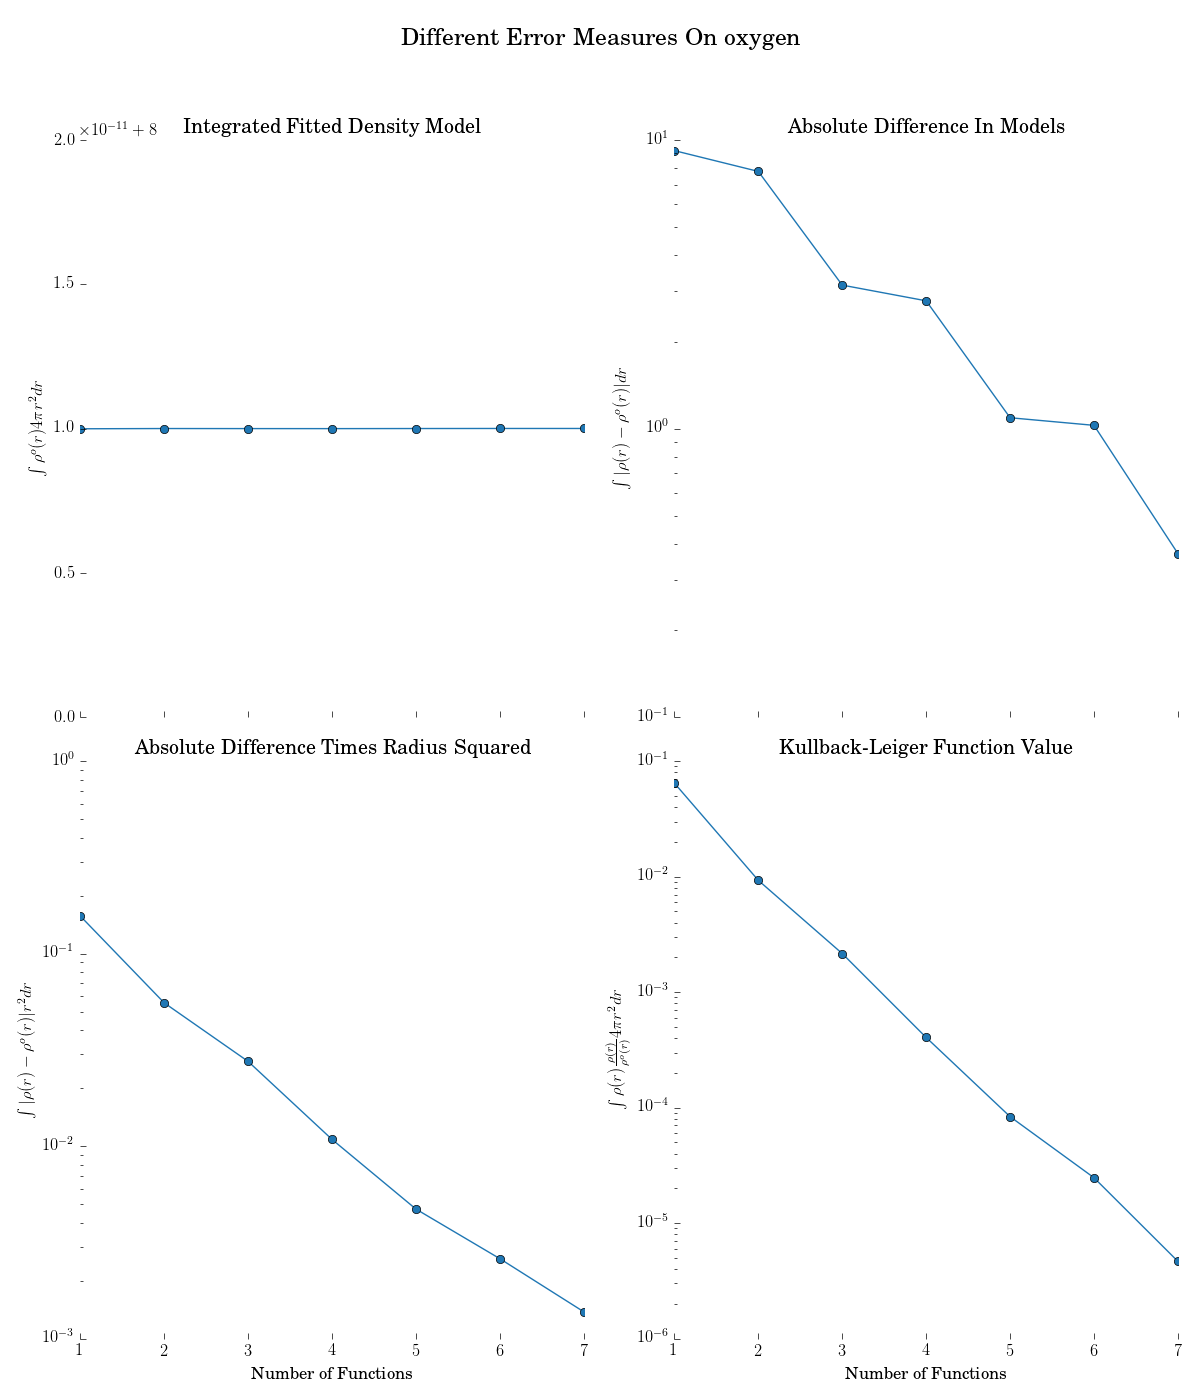
\includegraphics[scale=0.32]{results/o/error_plot_using_greedy-mbis.png}}
\fbox{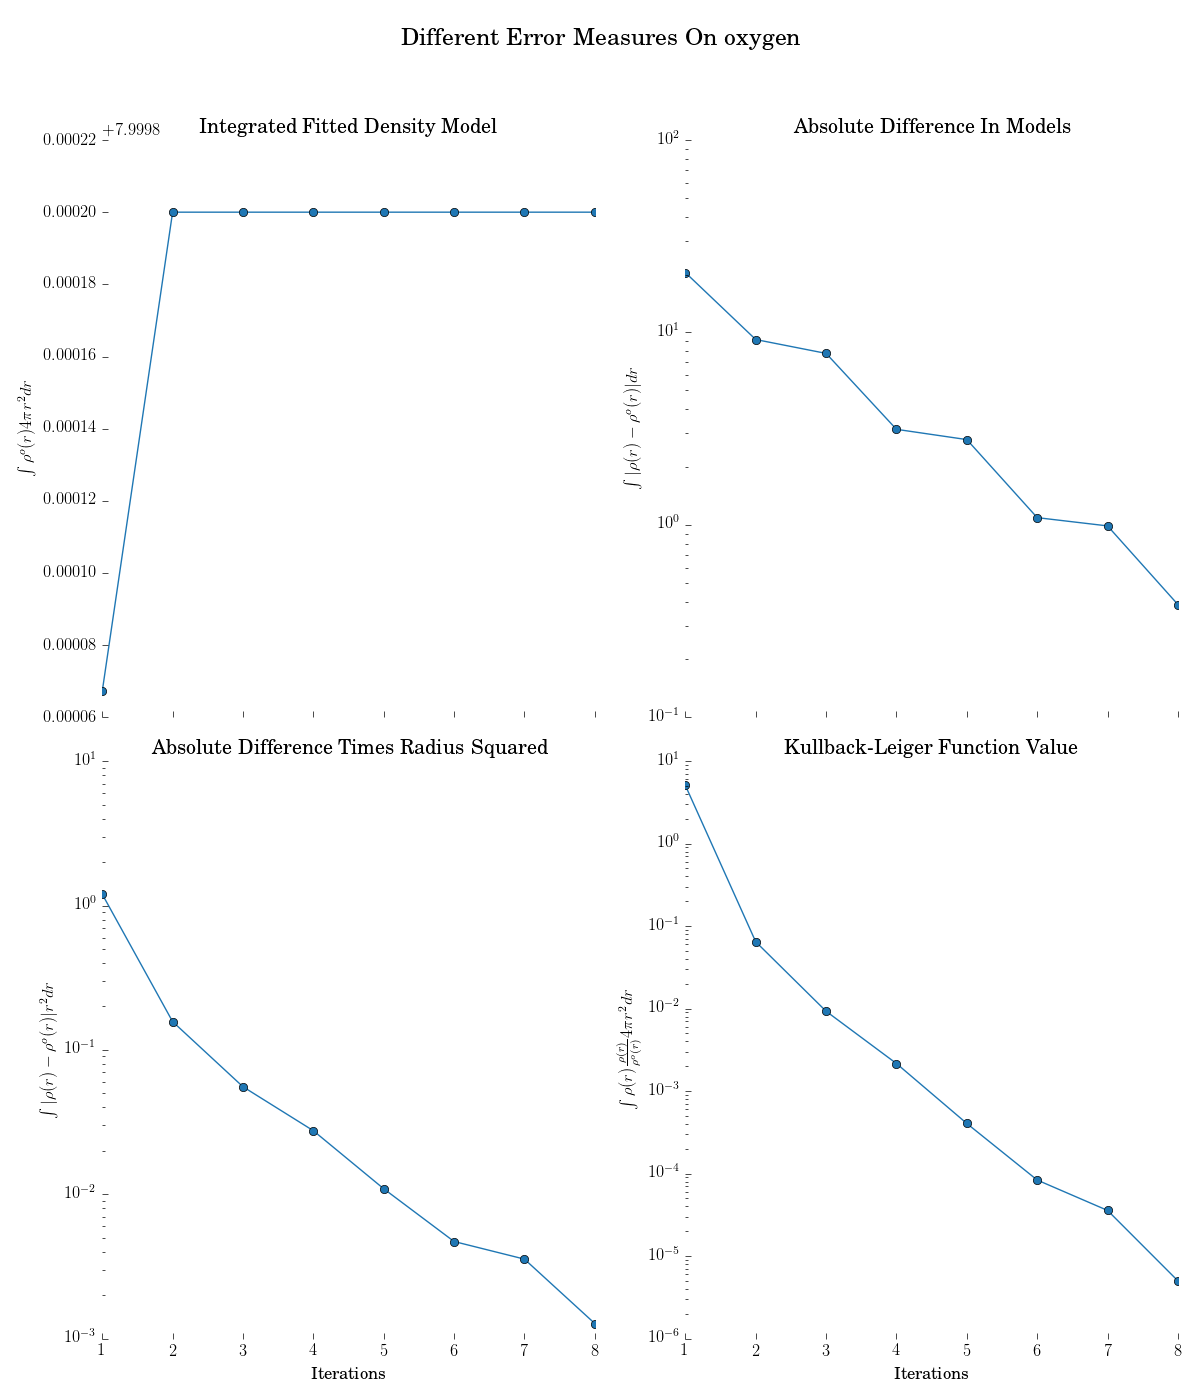
\includegraphics[scale=0.32]{results_original/o/error_plot_using_greedy-mbis.png}}
\fbox{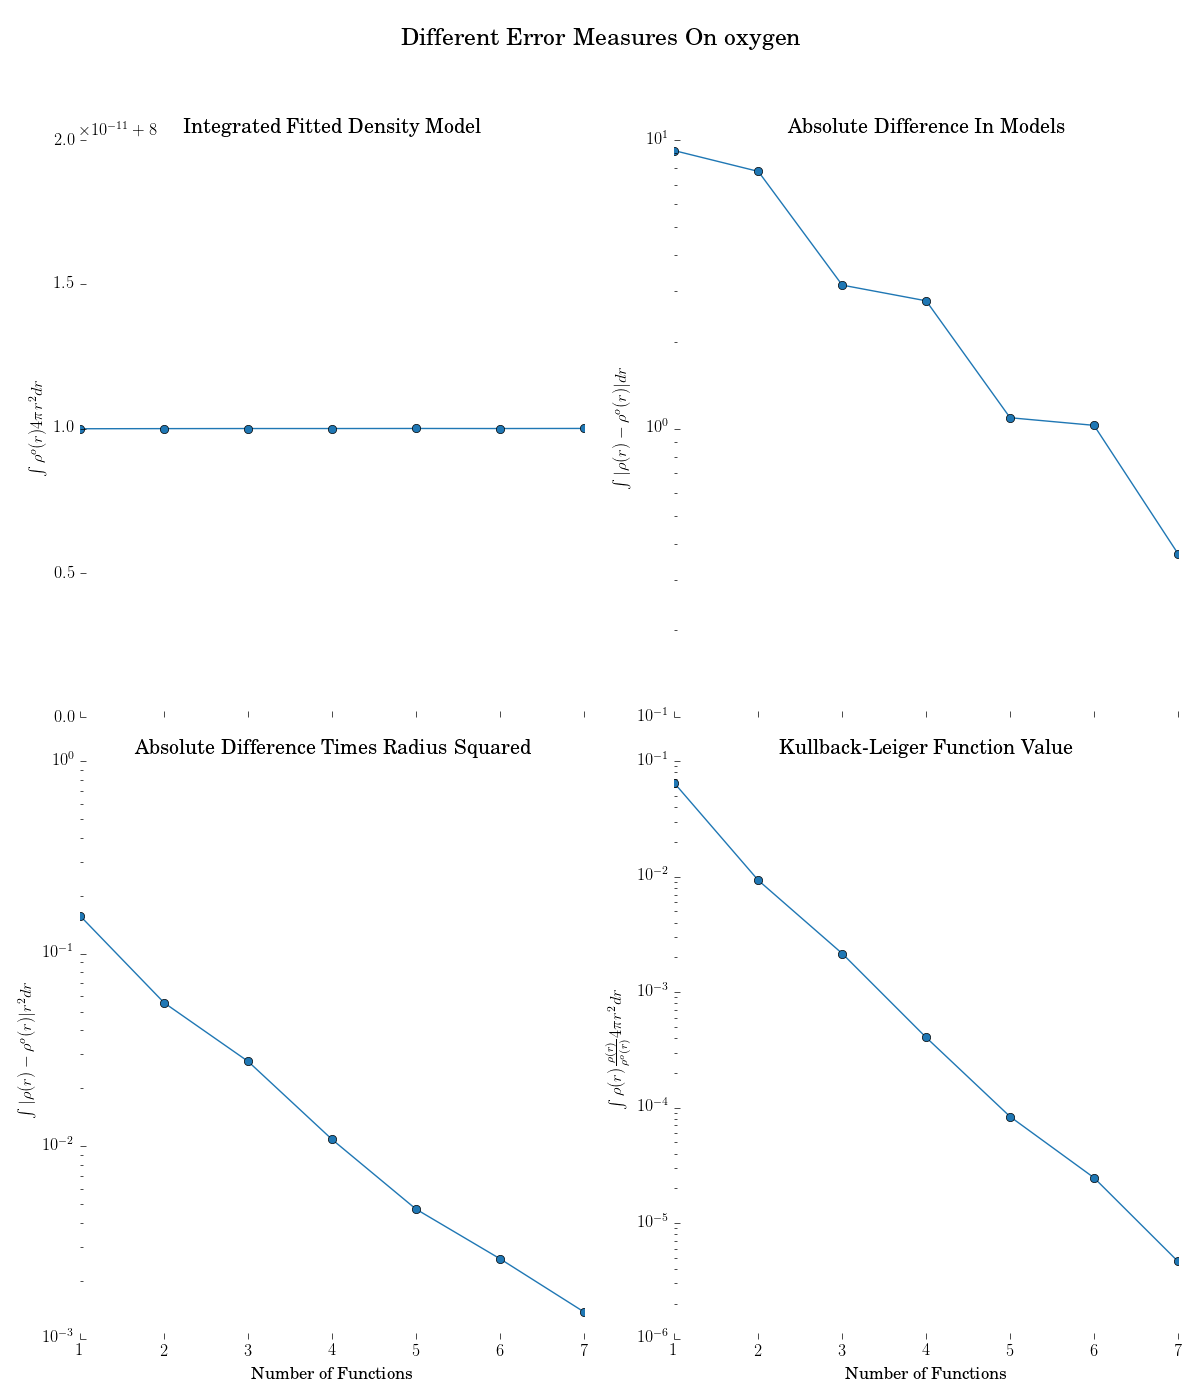
\includegraphics[scale=0.32]{results_redudancies/o/error_plot_using_greedy-mbis.png}}
\subsection{f}
\fbox{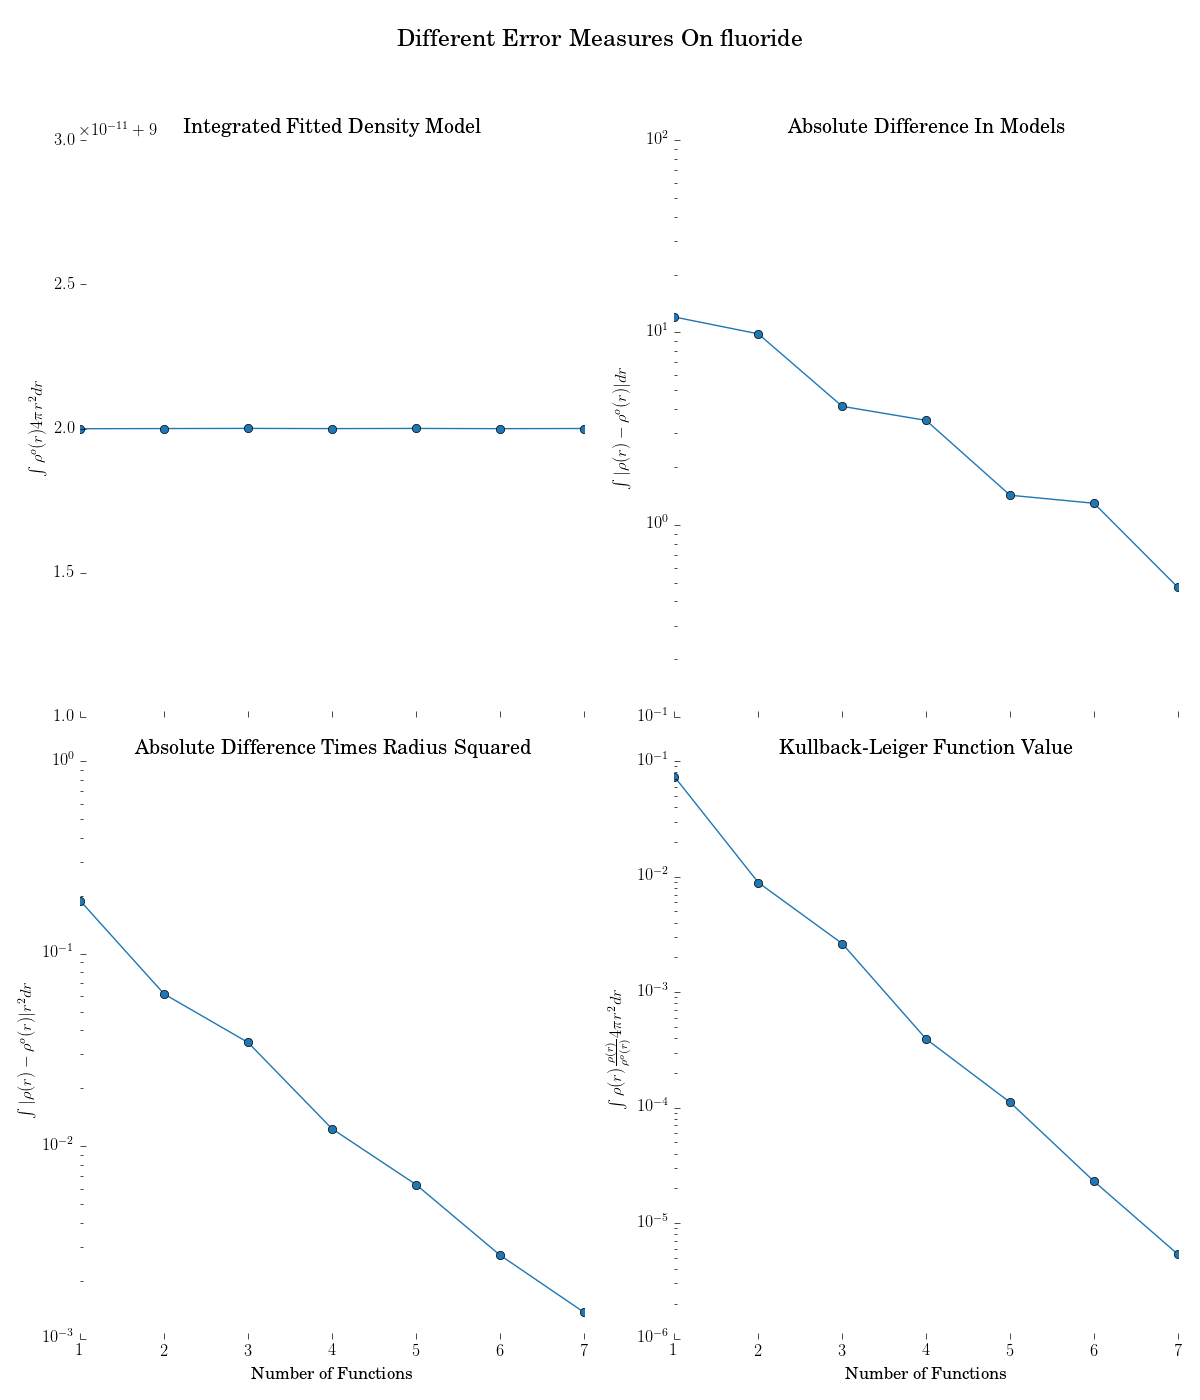
\includegraphics[scale=0.32]{results/f/error_plot_using_greedy-mbis.png}}
\fbox{\includegraphics[scale=0.32]{results_original/f/error_plot_using_greedy-mbis.png}}
\fbox{\includegraphics[scale=0.32]{results_redudancies/f/error_plot_using_greedy-mbis.png}}
\subsection{ne}
\fbox{\includegraphics[scale=0.32]{results/ne/error_plot_using_greedy-mbis.png}}
\fbox{\includegraphics[scale=0.32]{results_original/ne/error_plot_using_greedy-mbis.png}}
\fbox{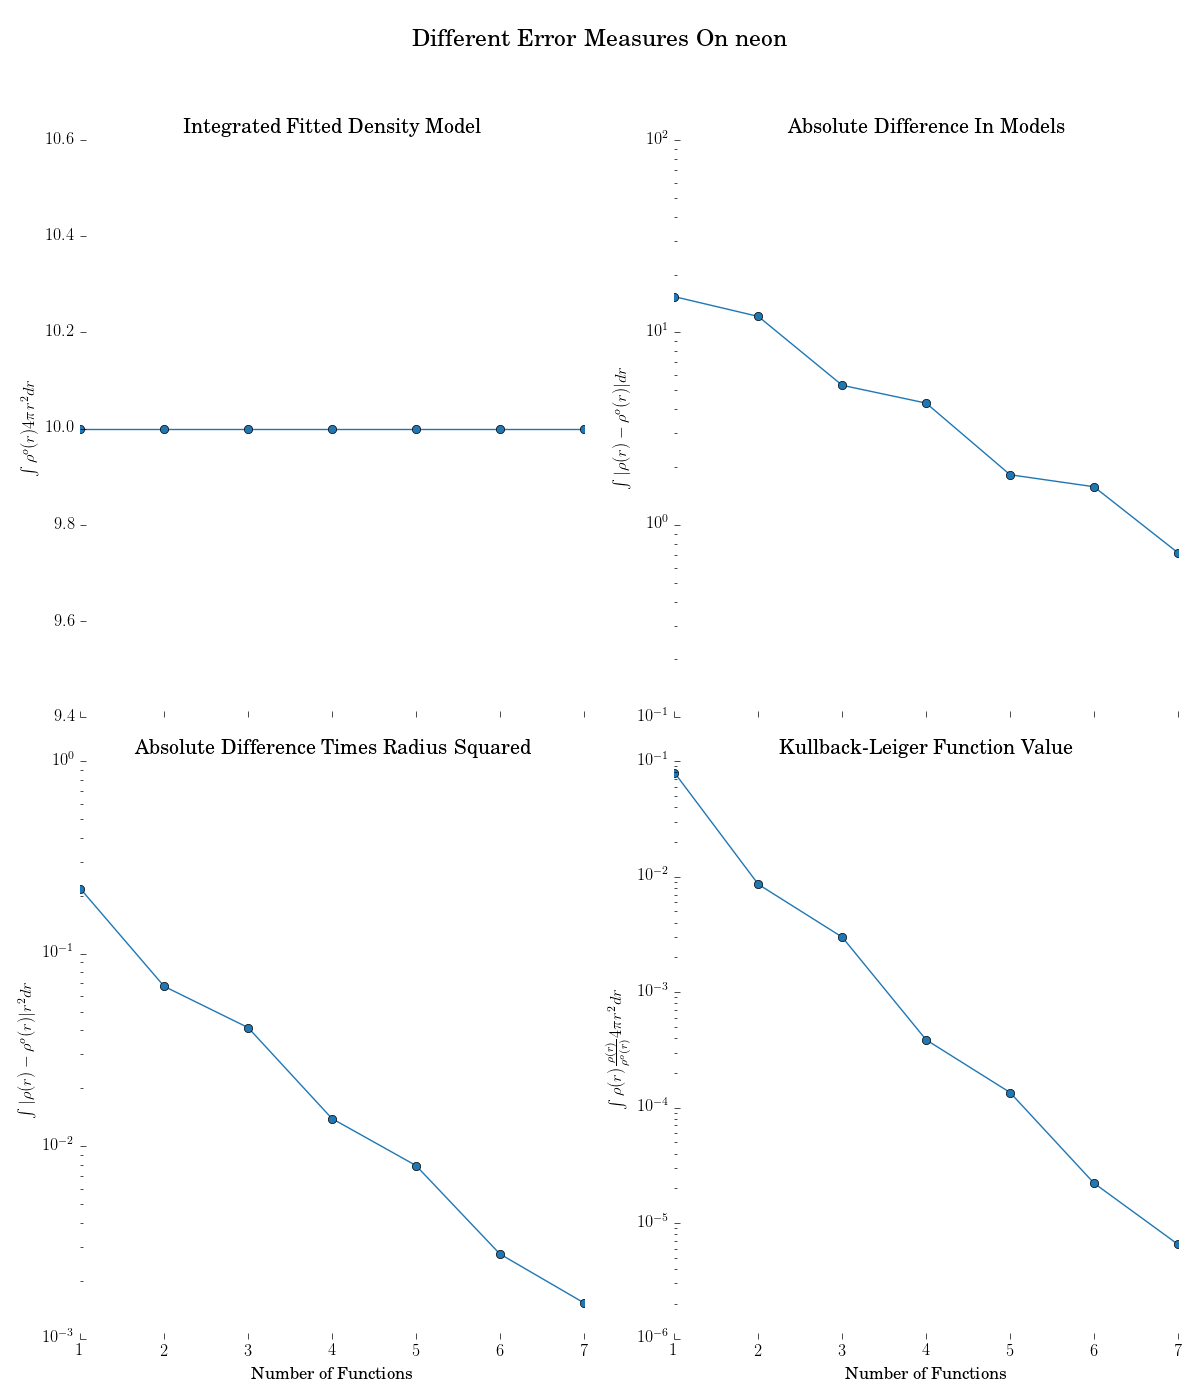
\includegraphics[scale=0.32]{results_redudancies/ne/error_plot_using_greedy-mbis.png}}


\section{Plotting Grouped By Method}
\subsection{Results Plots}
\fbox{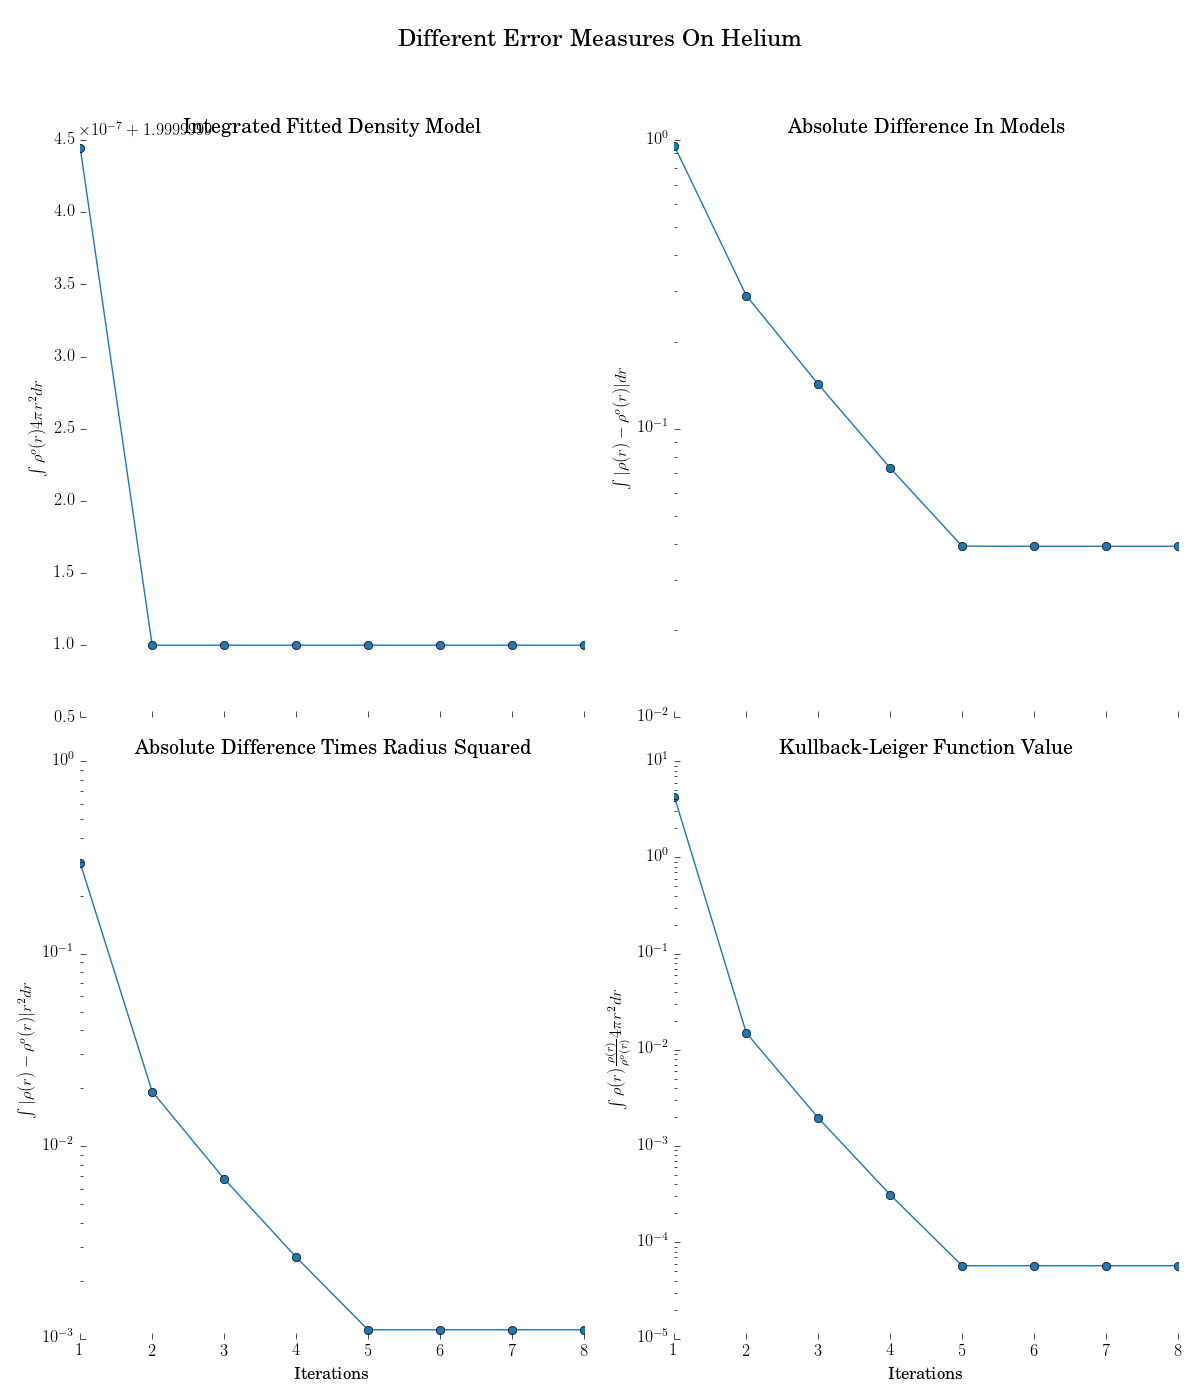
\includegraphics[scale=0.32]{results/he/error_plot_using_greedy-mbis.png}}
\fbox{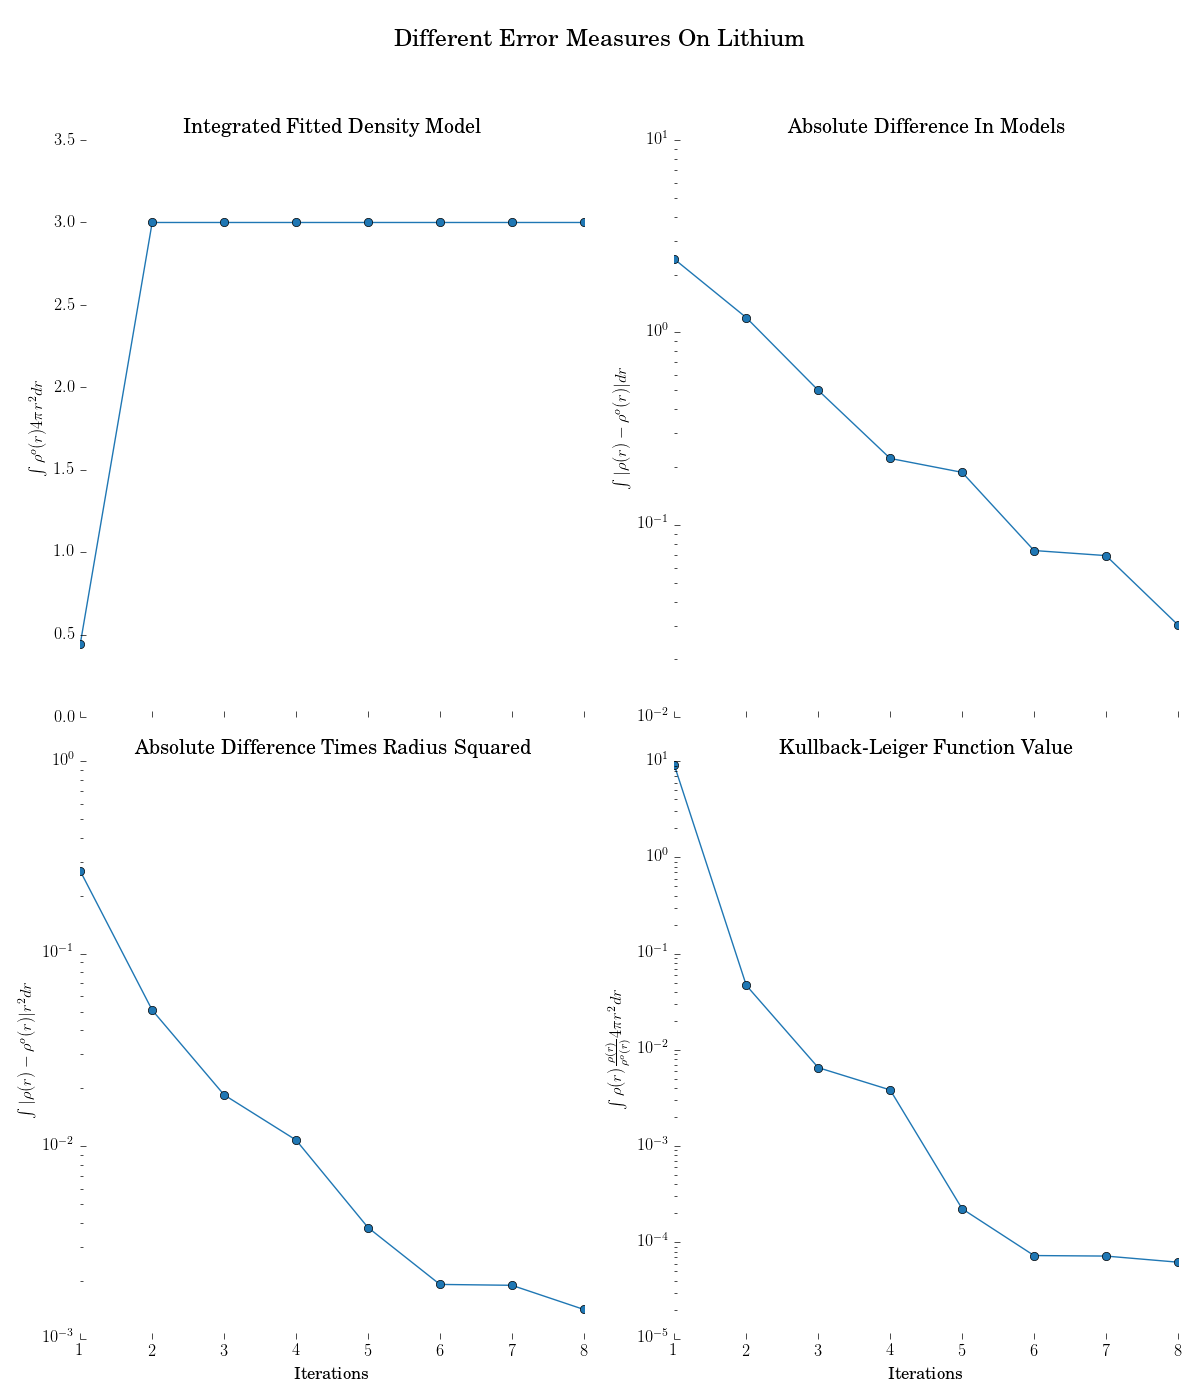
\includegraphics[scale=0.32]{results/li/error_plot_using_greedy-mbis.png}} \\
\fbox{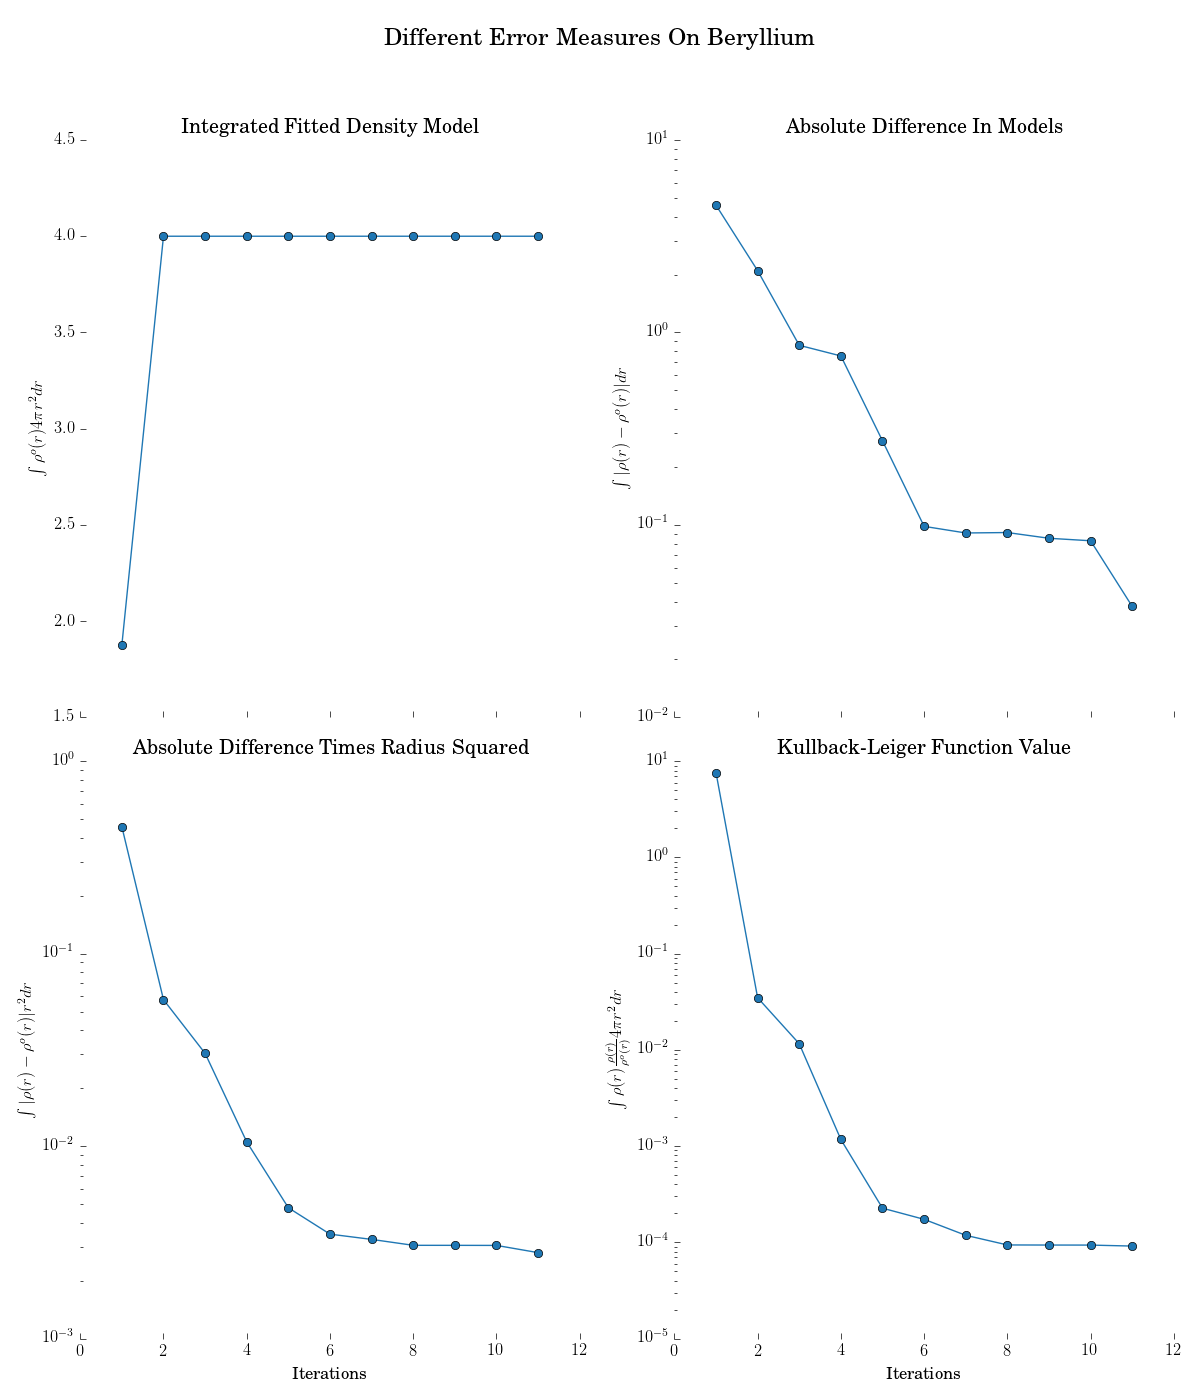
\includegraphics[scale=0.32]{results/be/error_plot_using_greedy-mbis.png}}
\fbox{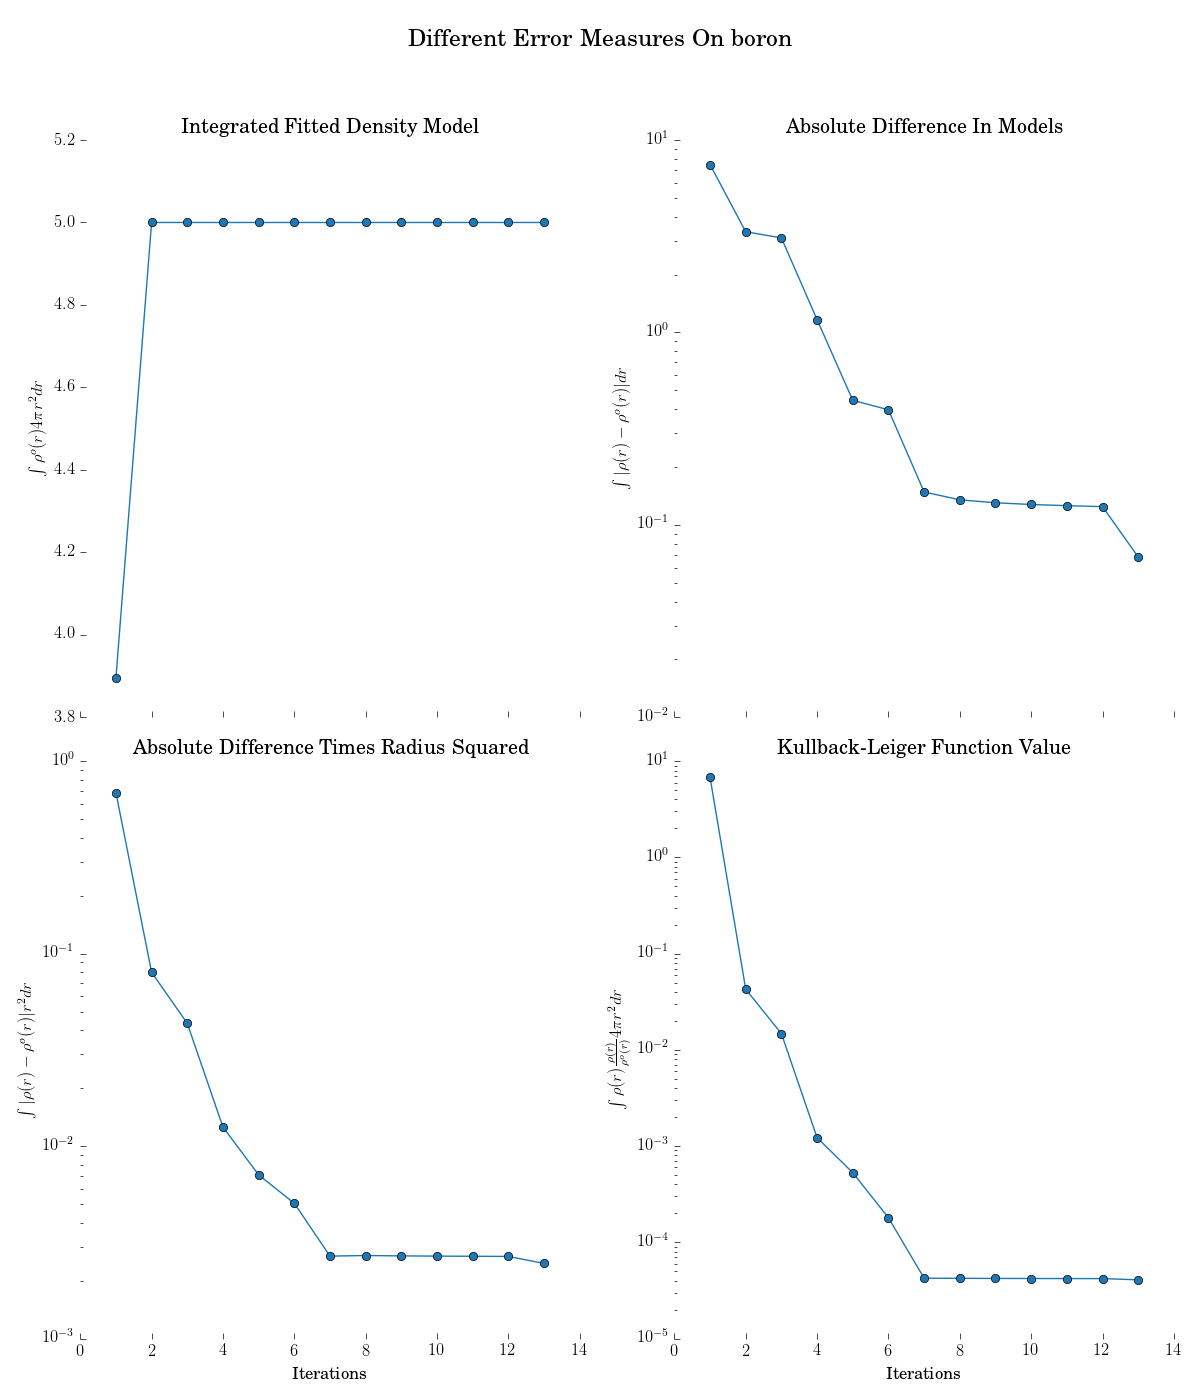
\includegraphics[scale=0.32]{results/b/error_plot_using_greedy-mbis.png}}
\fbox{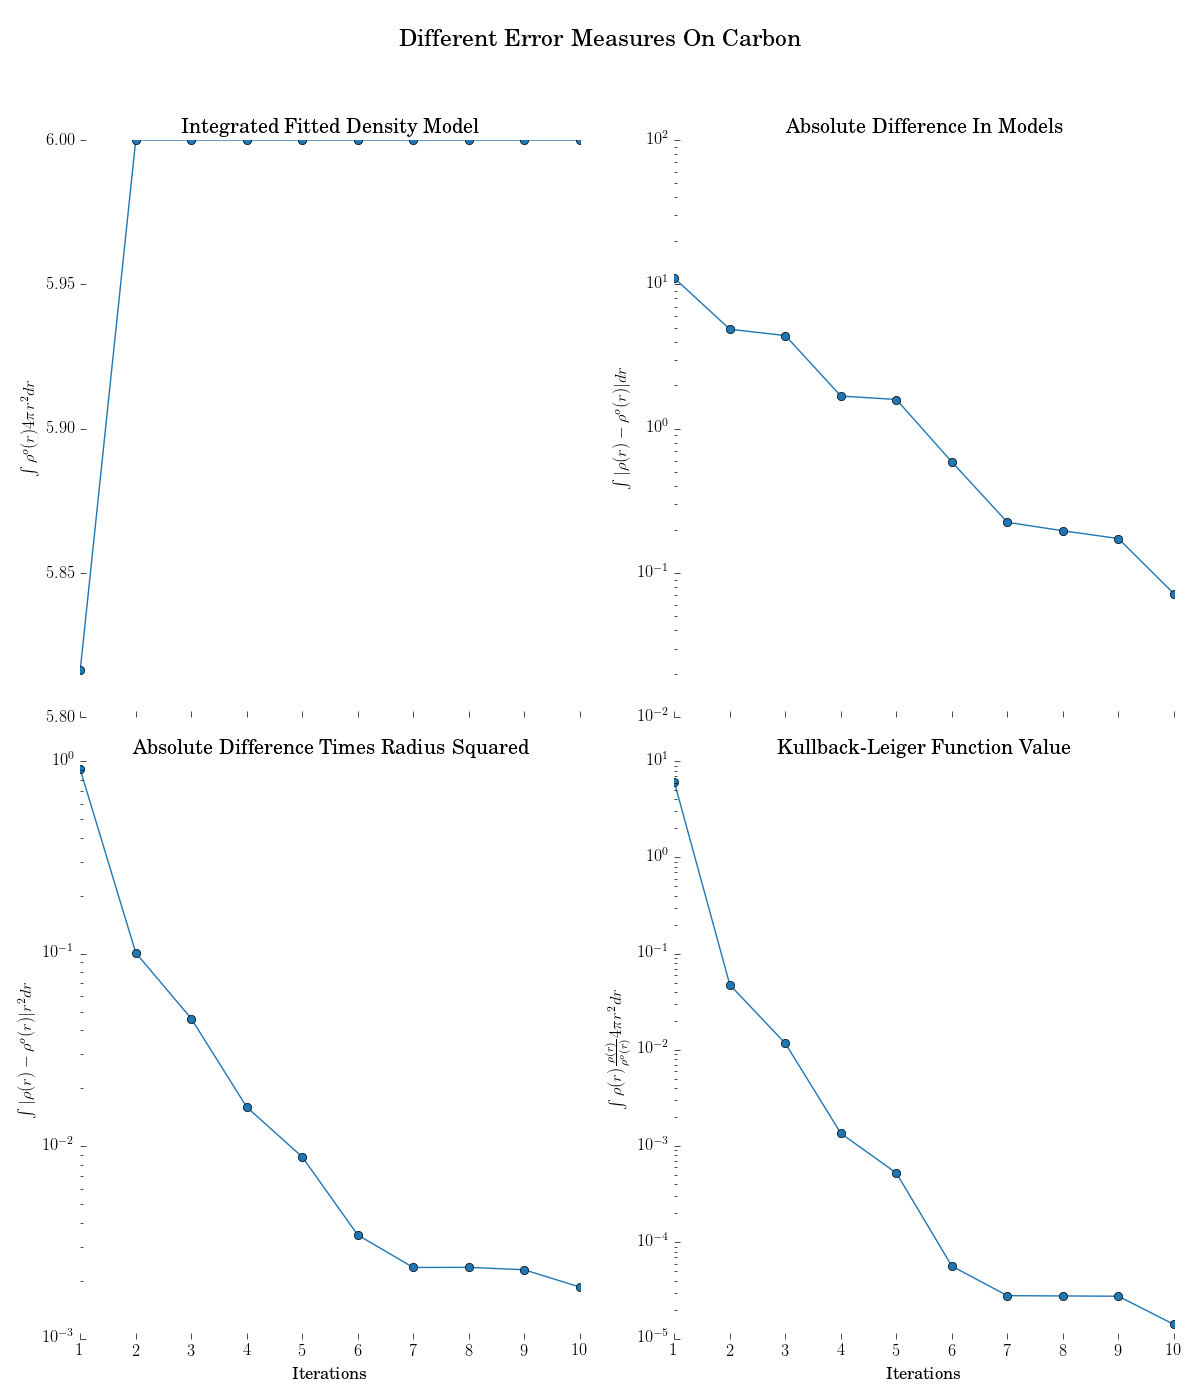
\includegraphics[scale=0.32]{results/c/error_plot_using_greedy-mbis.png}}
\fbox{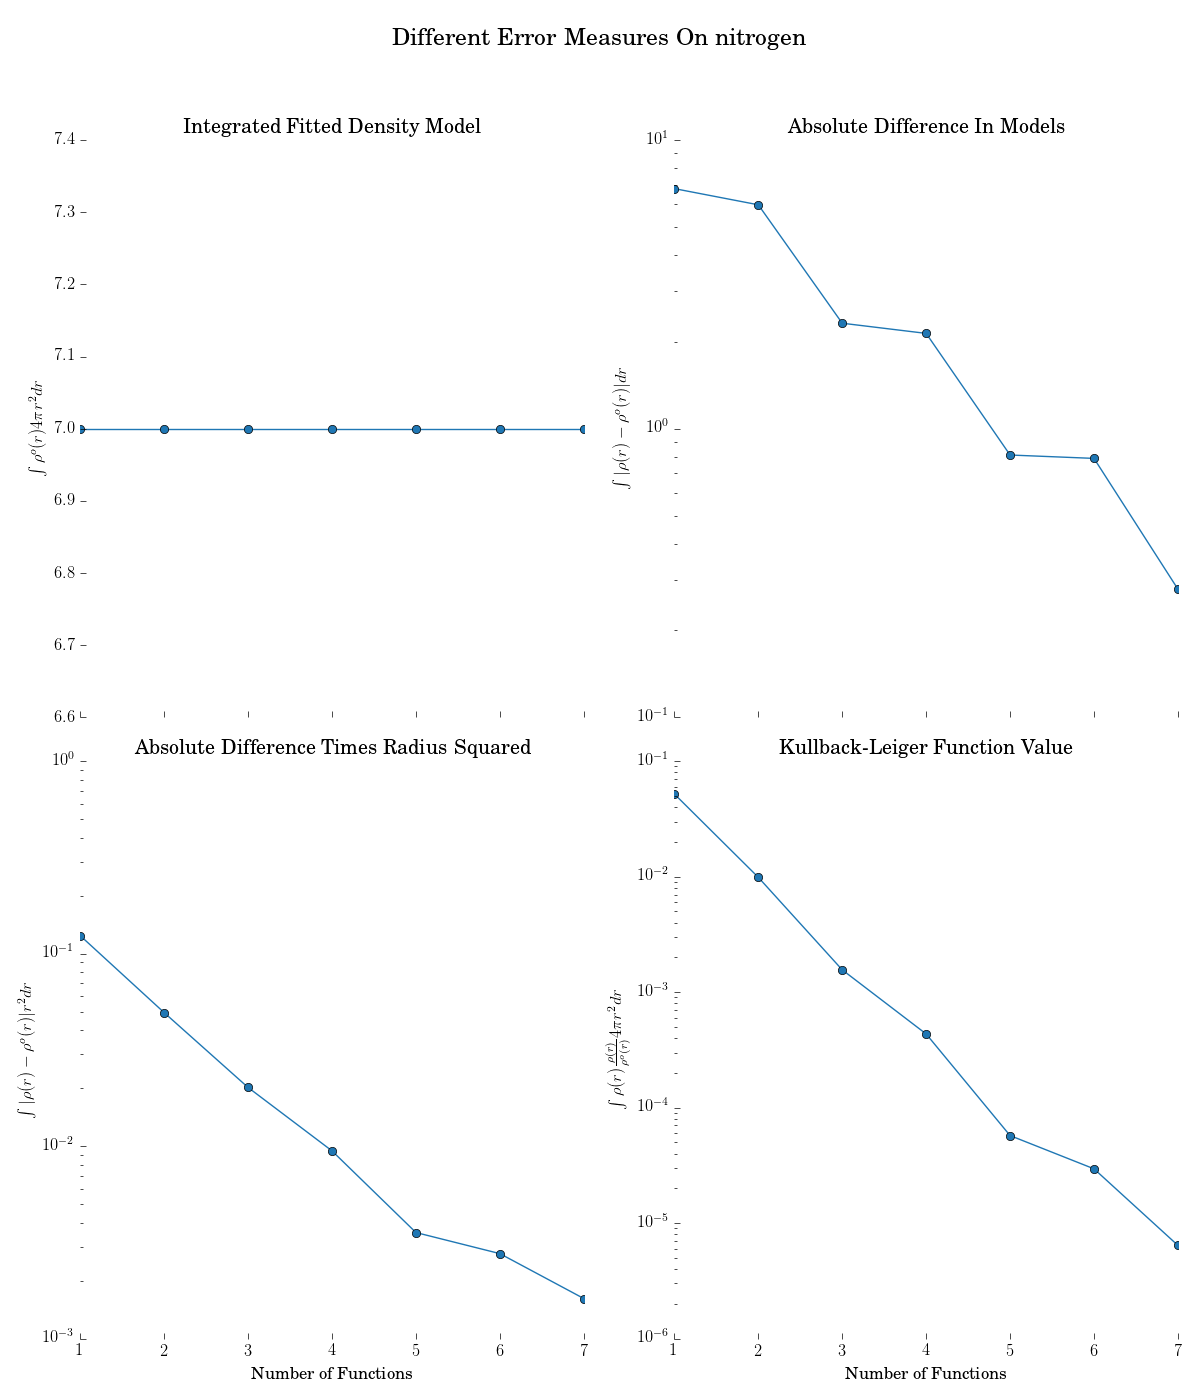
\includegraphics[scale=0.32]{results/n/error_plot_using_greedy-mbis.png}}\\
\fbox{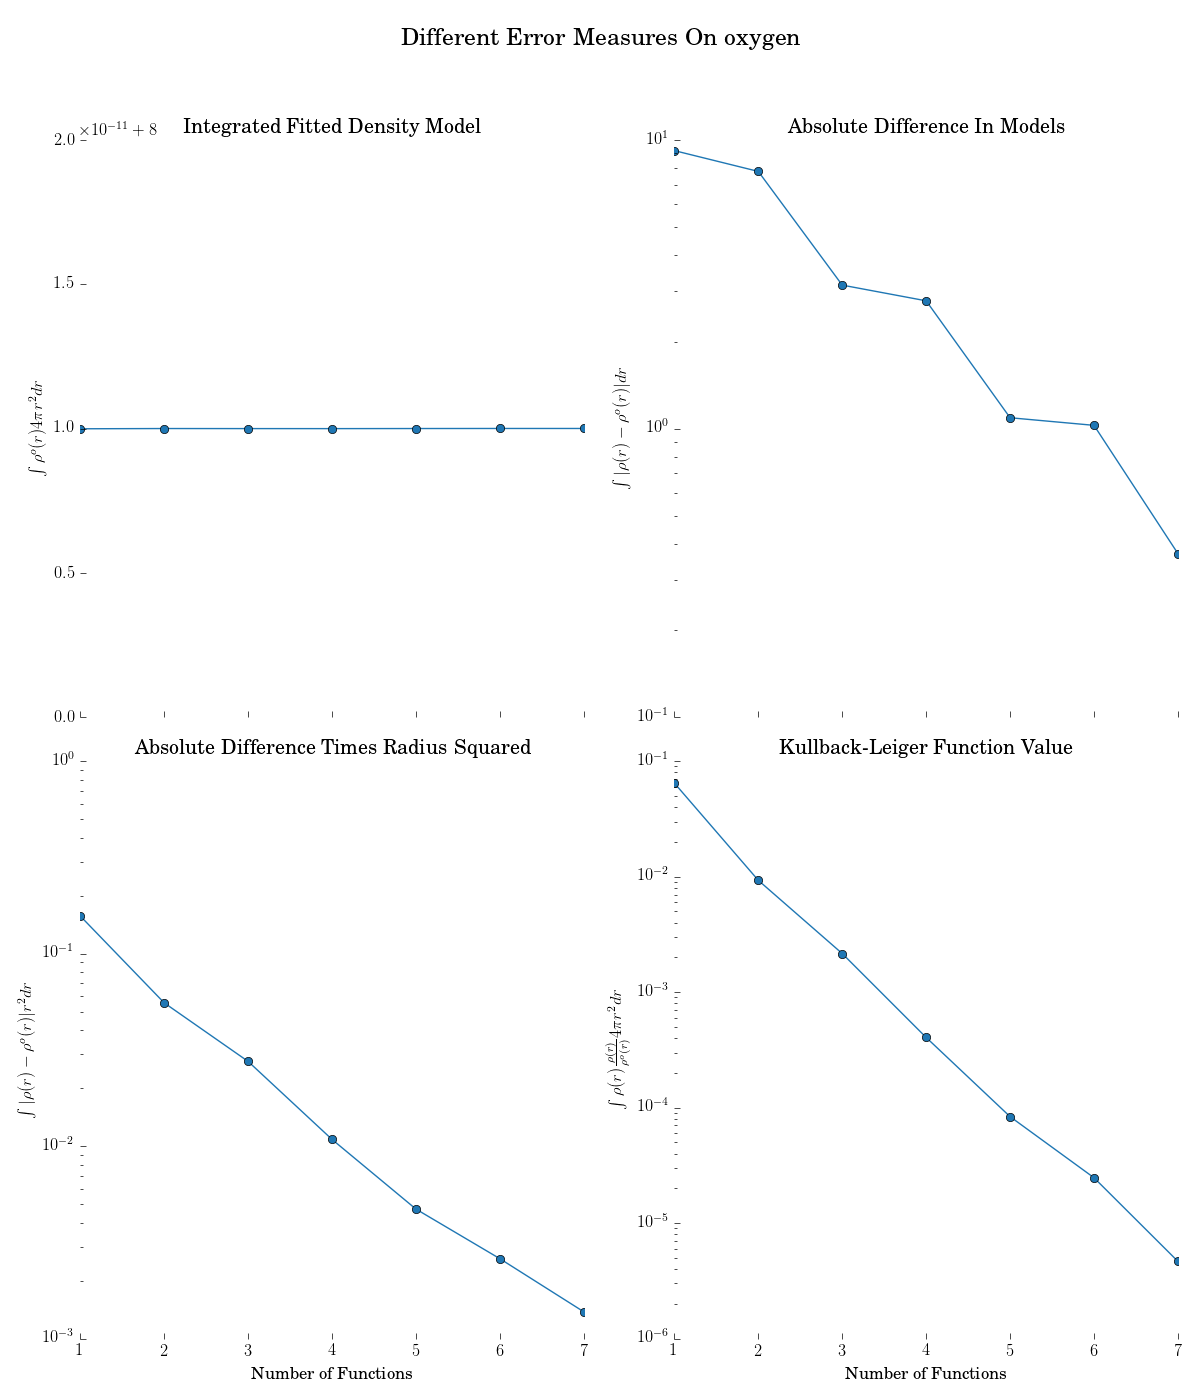
\includegraphics[scale=0.32]{results/o/error_plot_using_greedy-mbis.png}}
\fbox{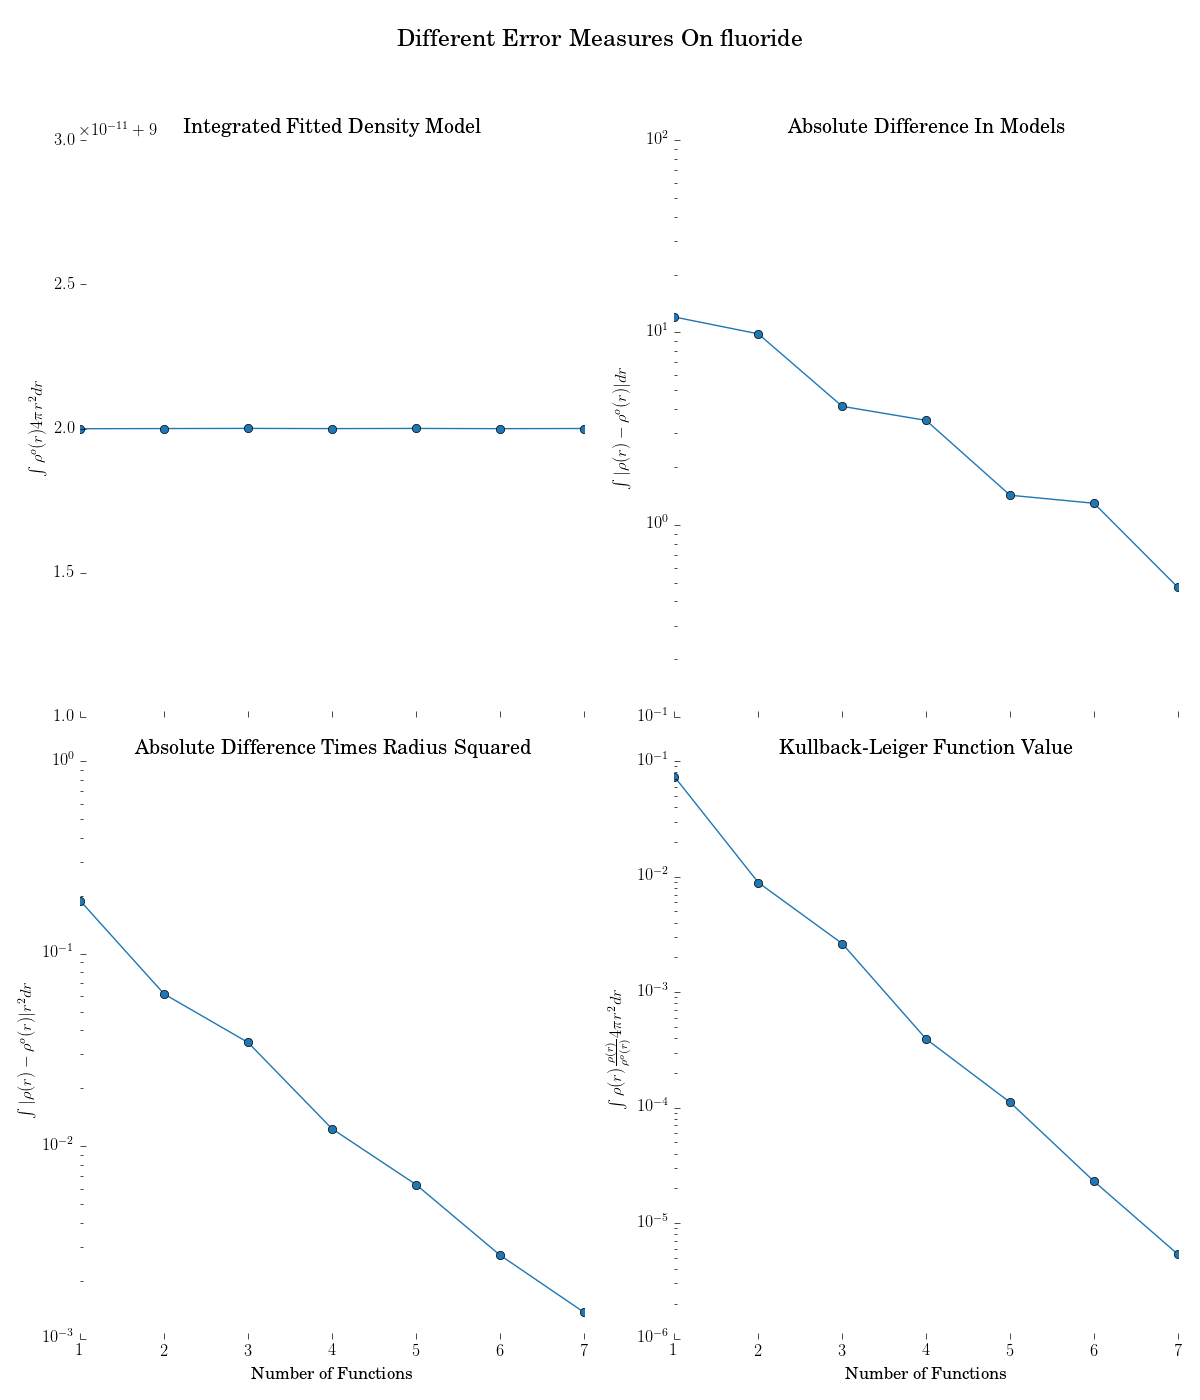
\includegraphics[scale=0.32]{results/f/error_plot_using_greedy-mbis.png}}\\
\fbox{\includegraphics[scale=0.32]{results/ne/error_plot_using_greedy-mbis.png}}\\

\subsection{Results\textunderscore Original Plots (X-Axis is Number of Basis Functions)}
\fbox{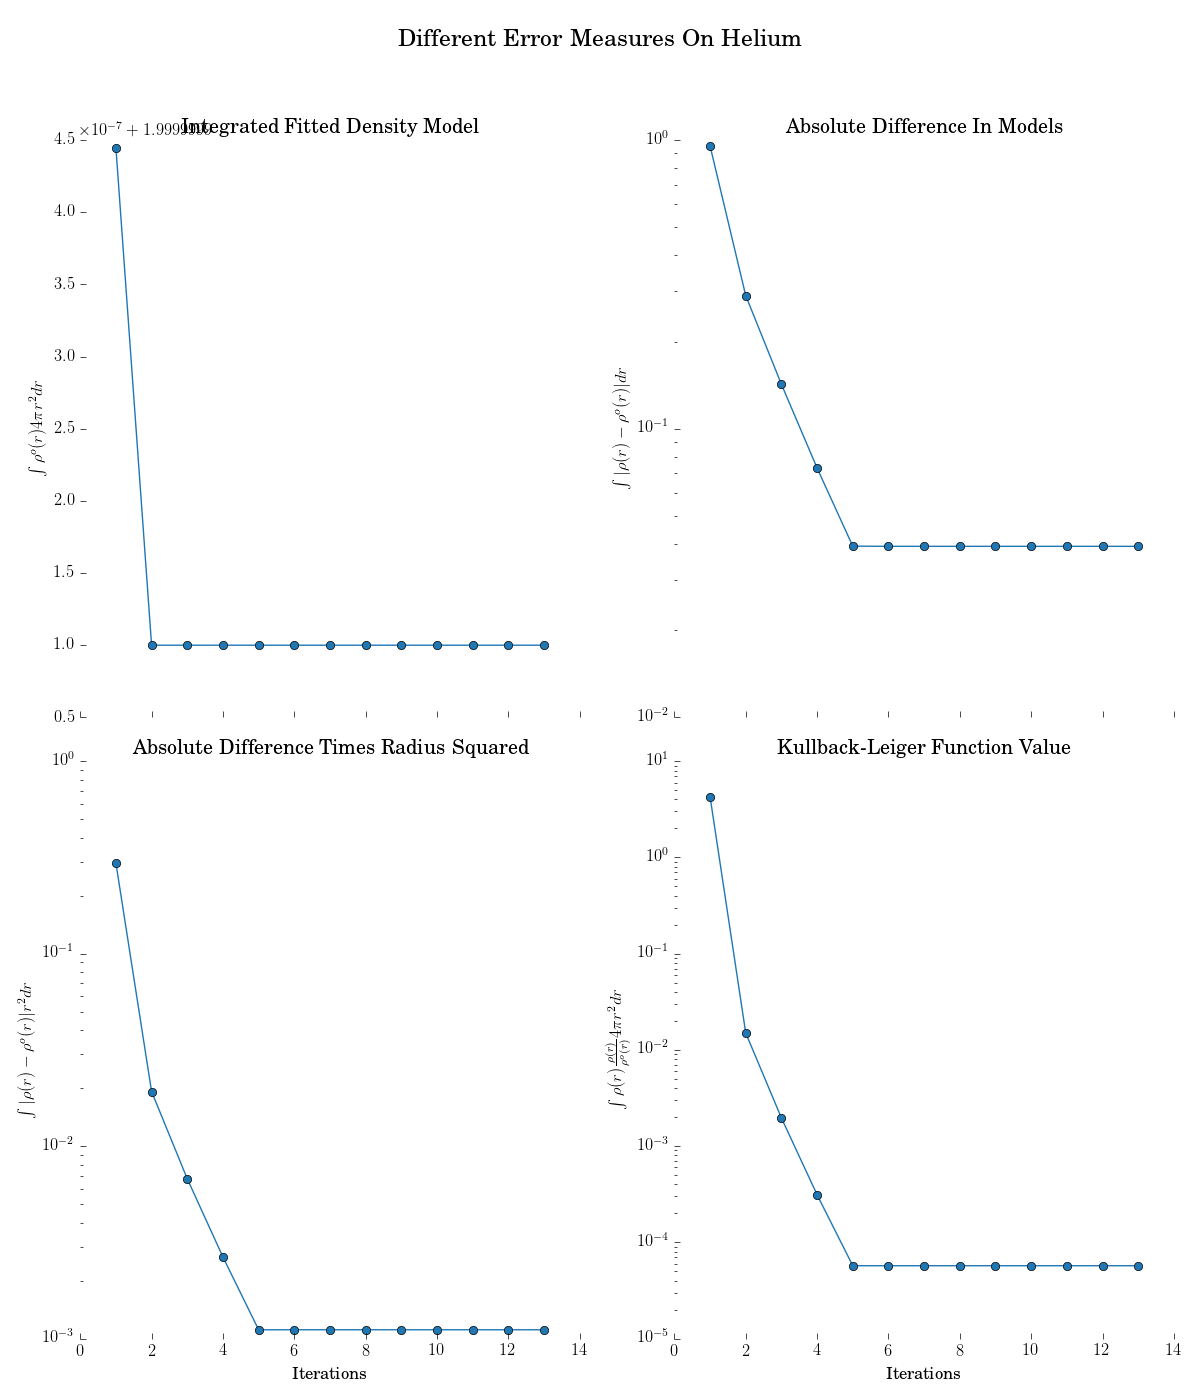
\includegraphics[scale=0.32]{results_original/he/error_plot_using_greedy-mbis.png}}
\fbox{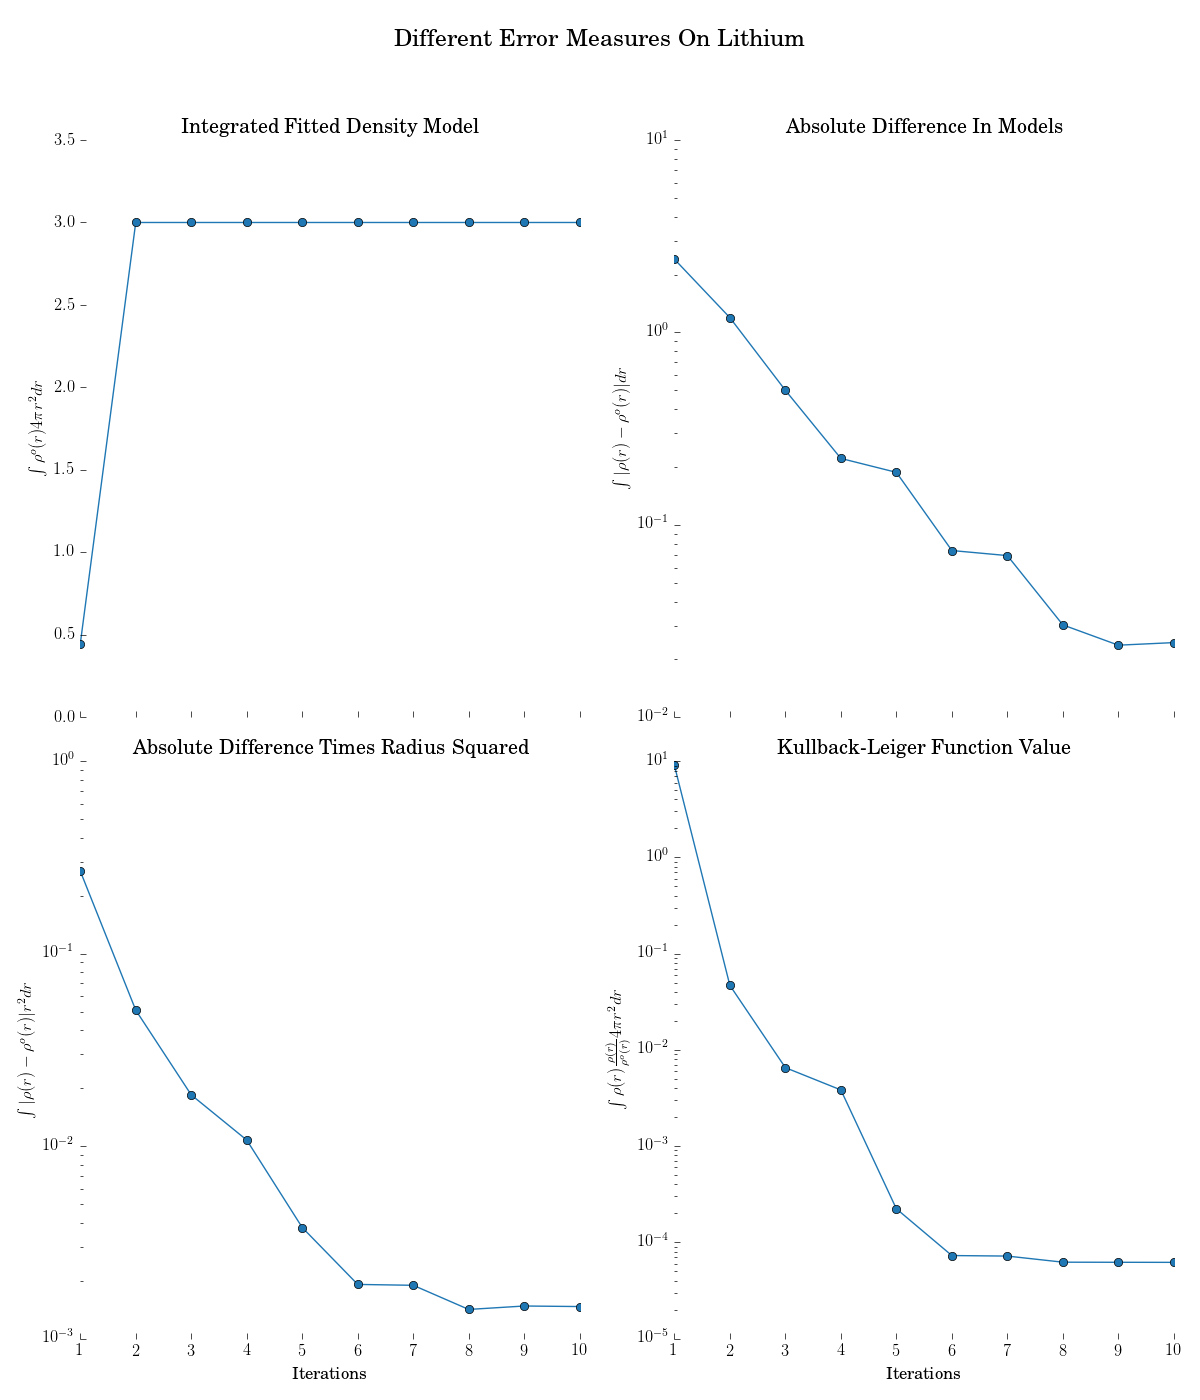
\includegraphics[scale=0.32]{results_original/li/error_plot_using_greedy-mbis.png}} \\
\fbox{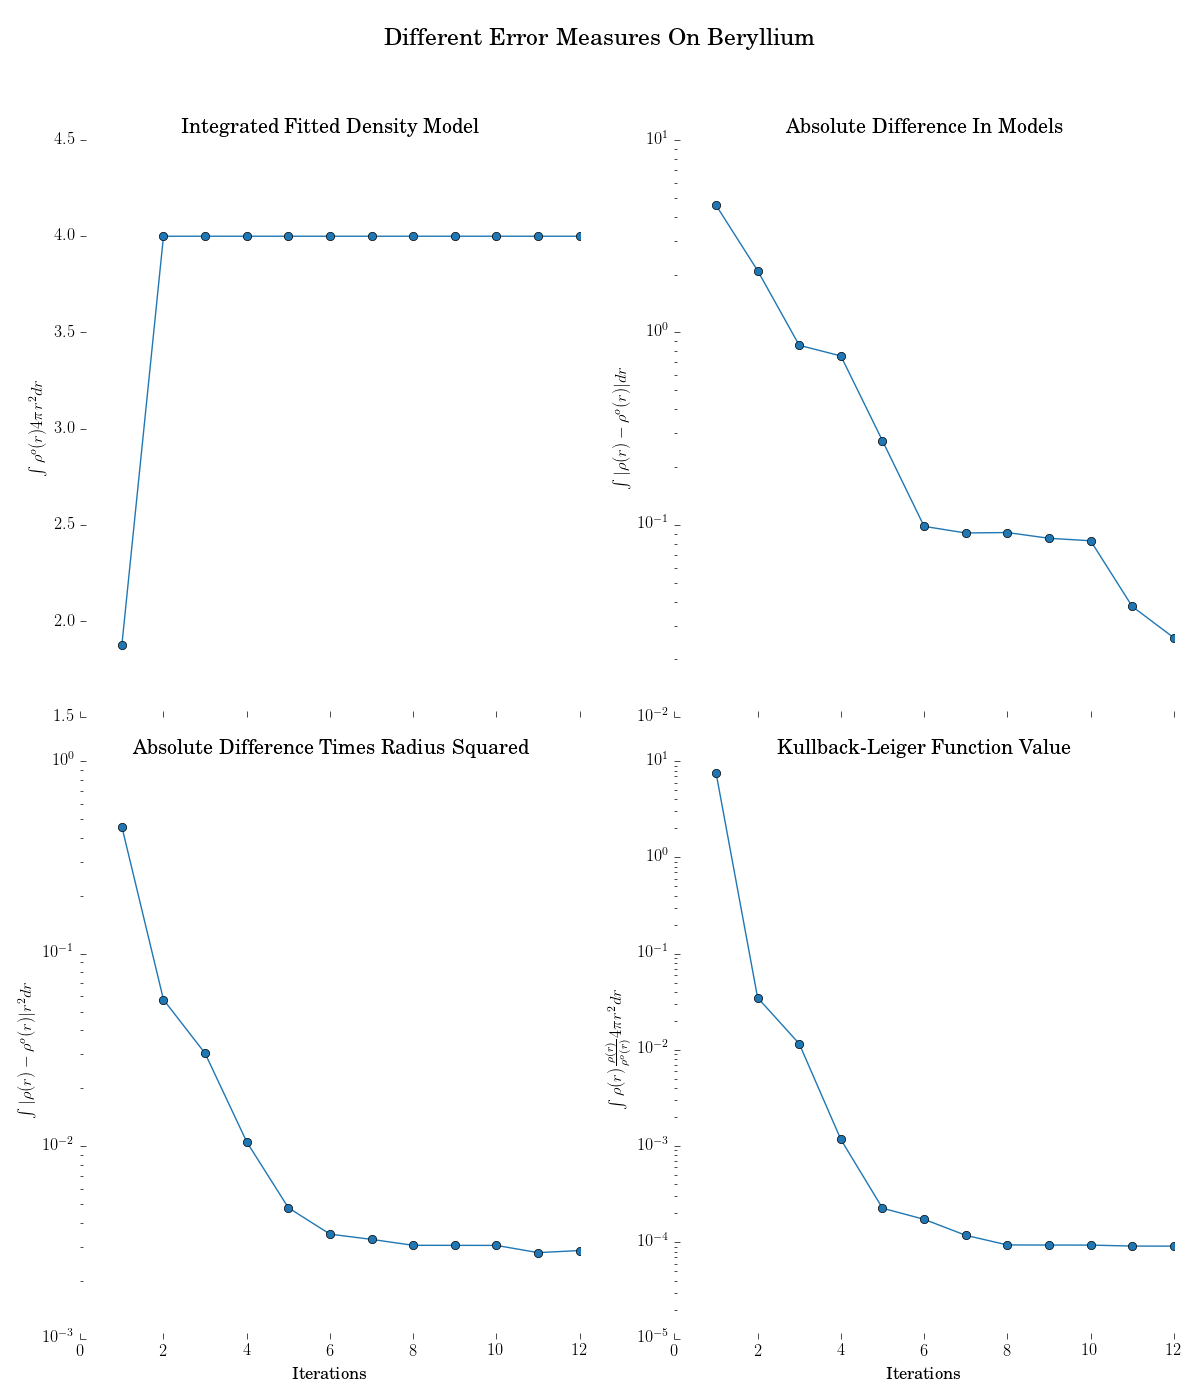
\includegraphics[scale=0.32]{results_original/be/error_plot_using_greedy-mbis.png}}
\fbox{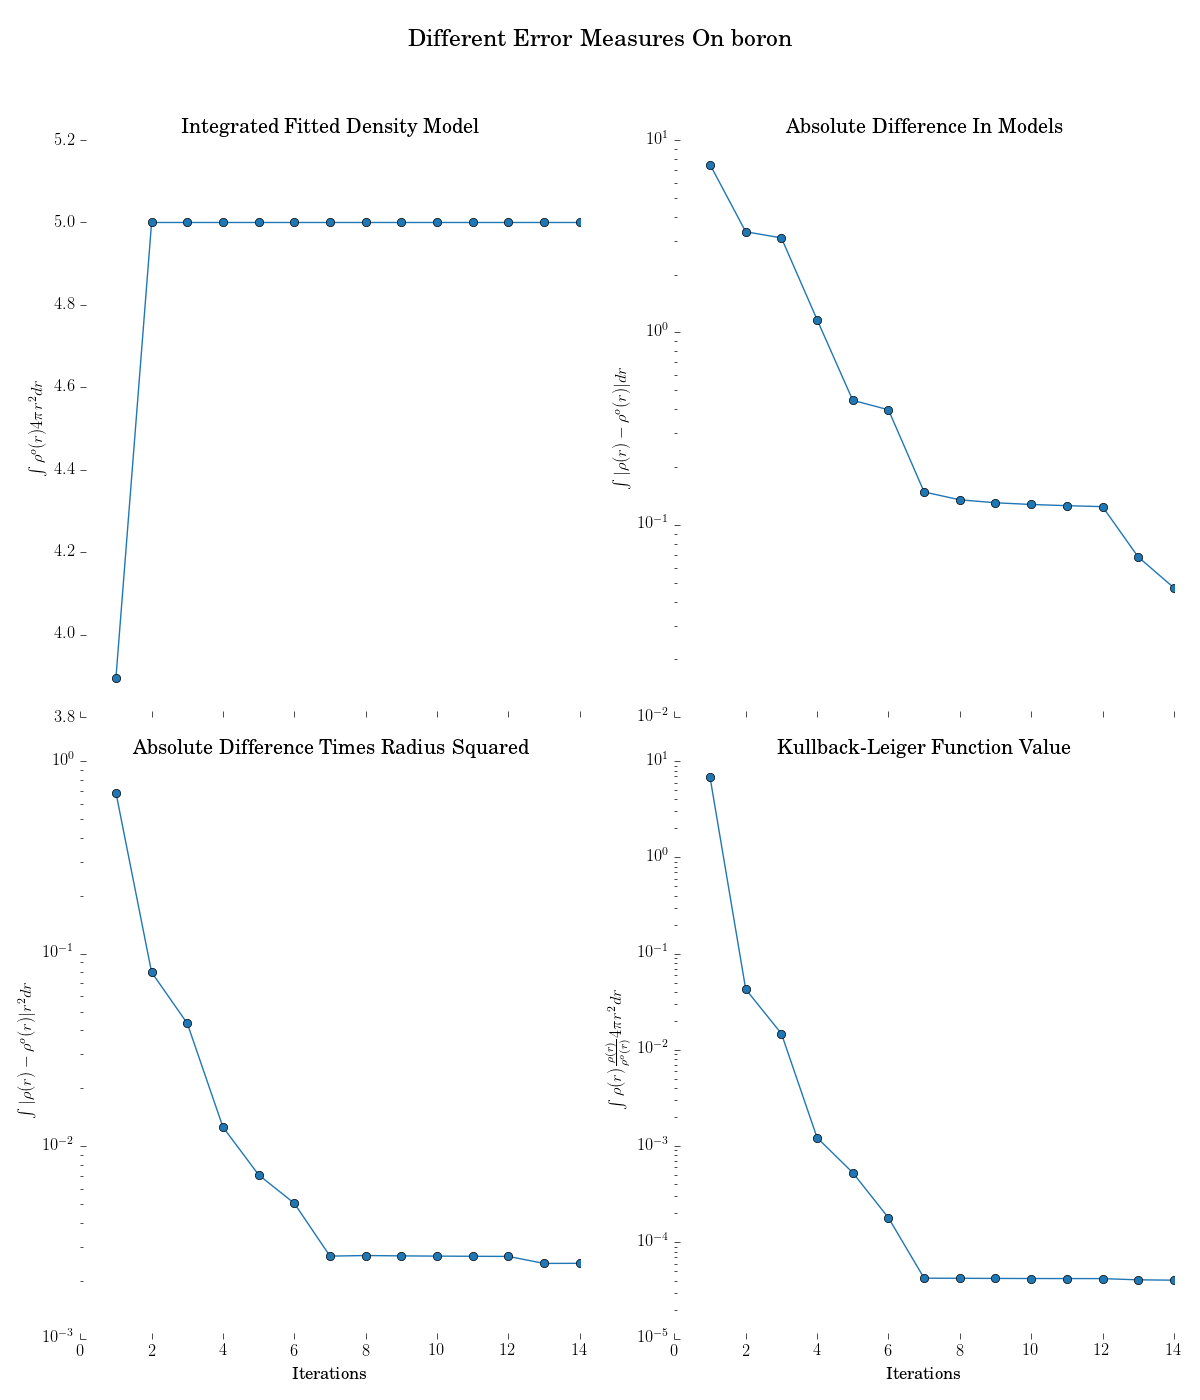
\includegraphics[scale=0.32]{results_original/b/error_plot_using_greedy-mbis.png}}
\fbox{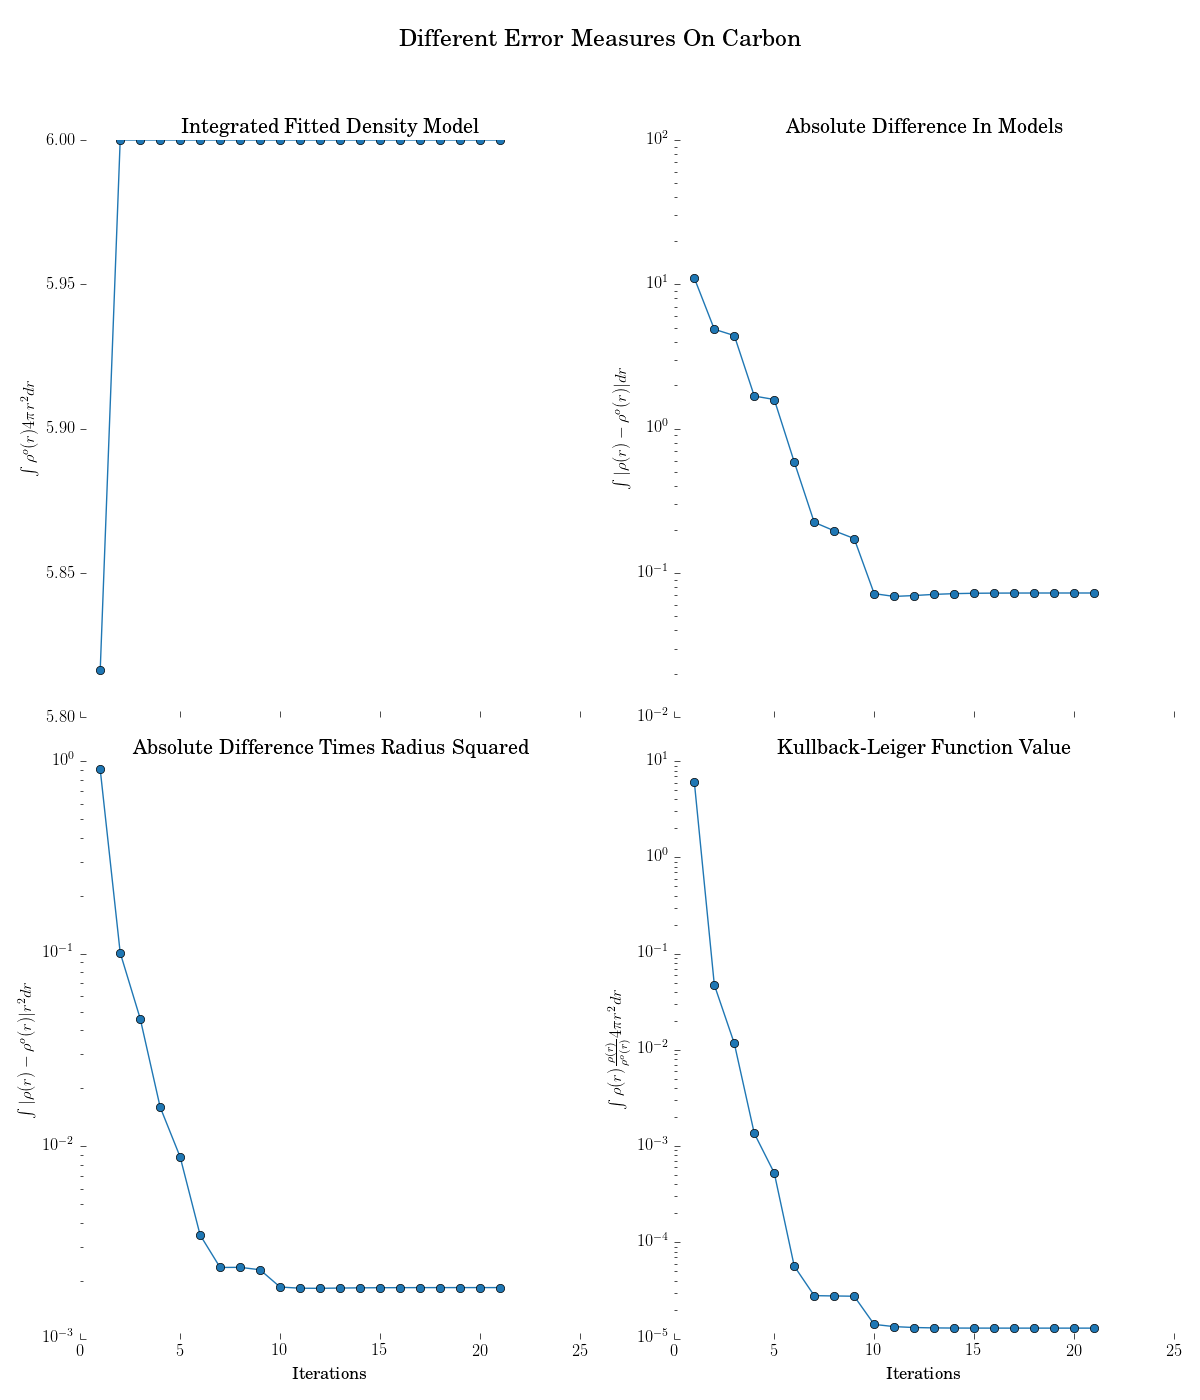
\includegraphics[scale=0.32]{results_original/c/error_plot_using_greedy-mbis.png}}
\fbox{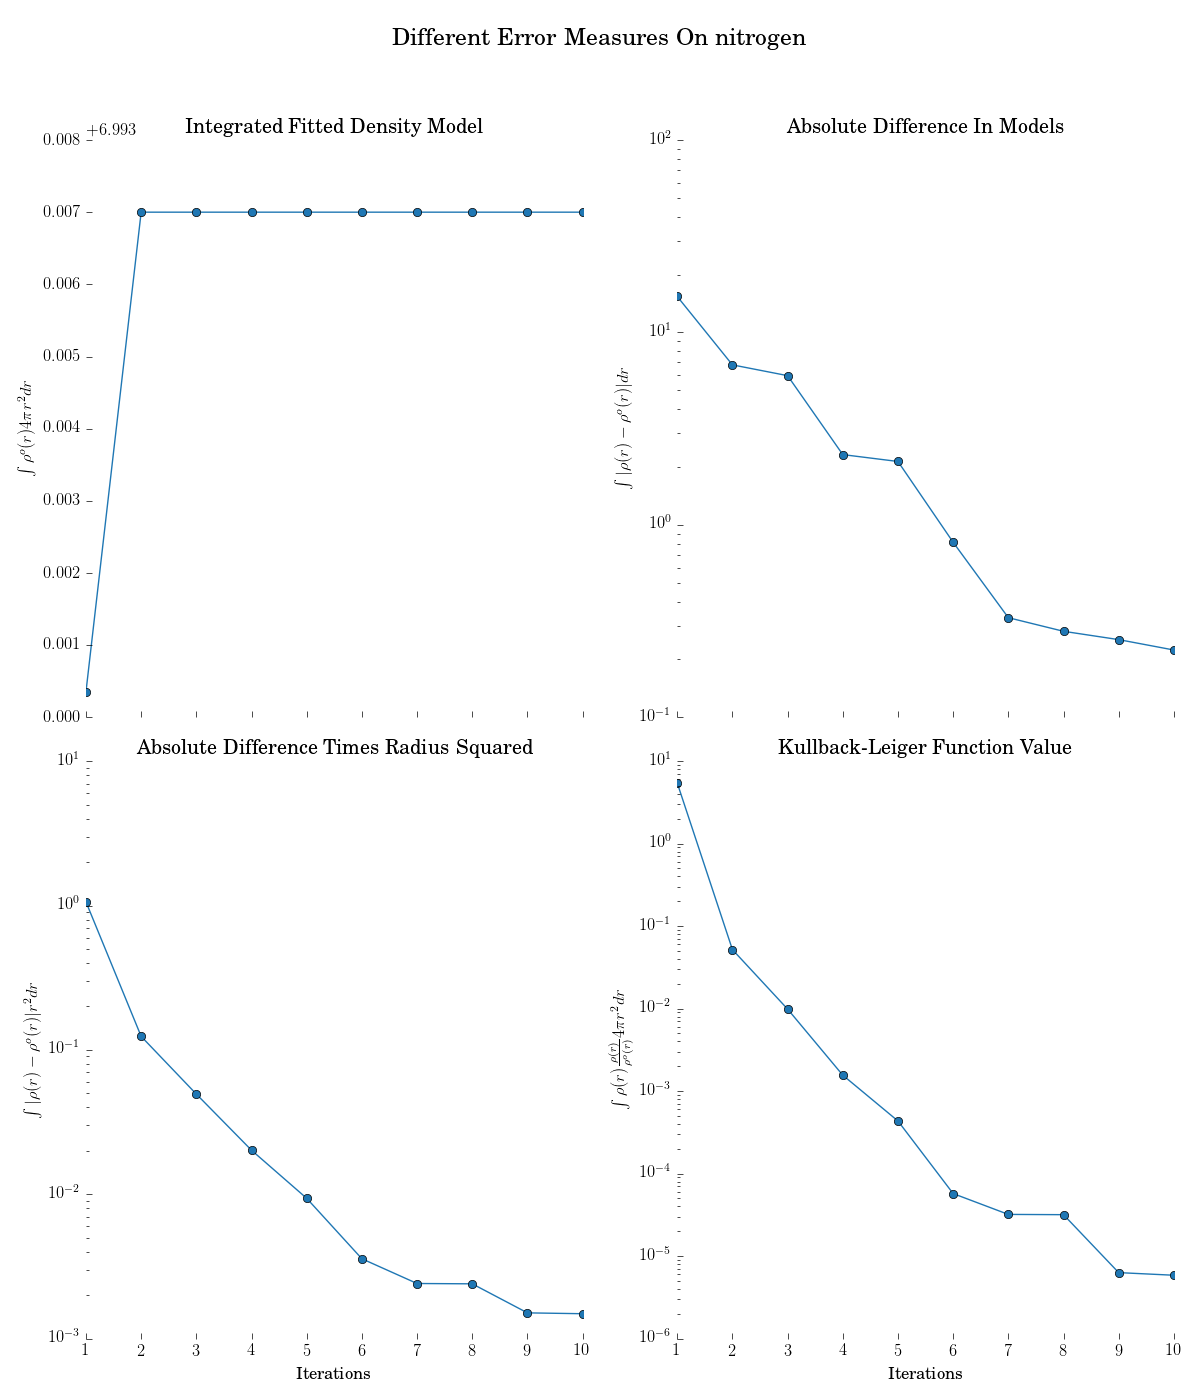
\includegraphics[scale=0.32]{results_original/n/error_plot_using_greedy-mbis.png}}\\
\fbox{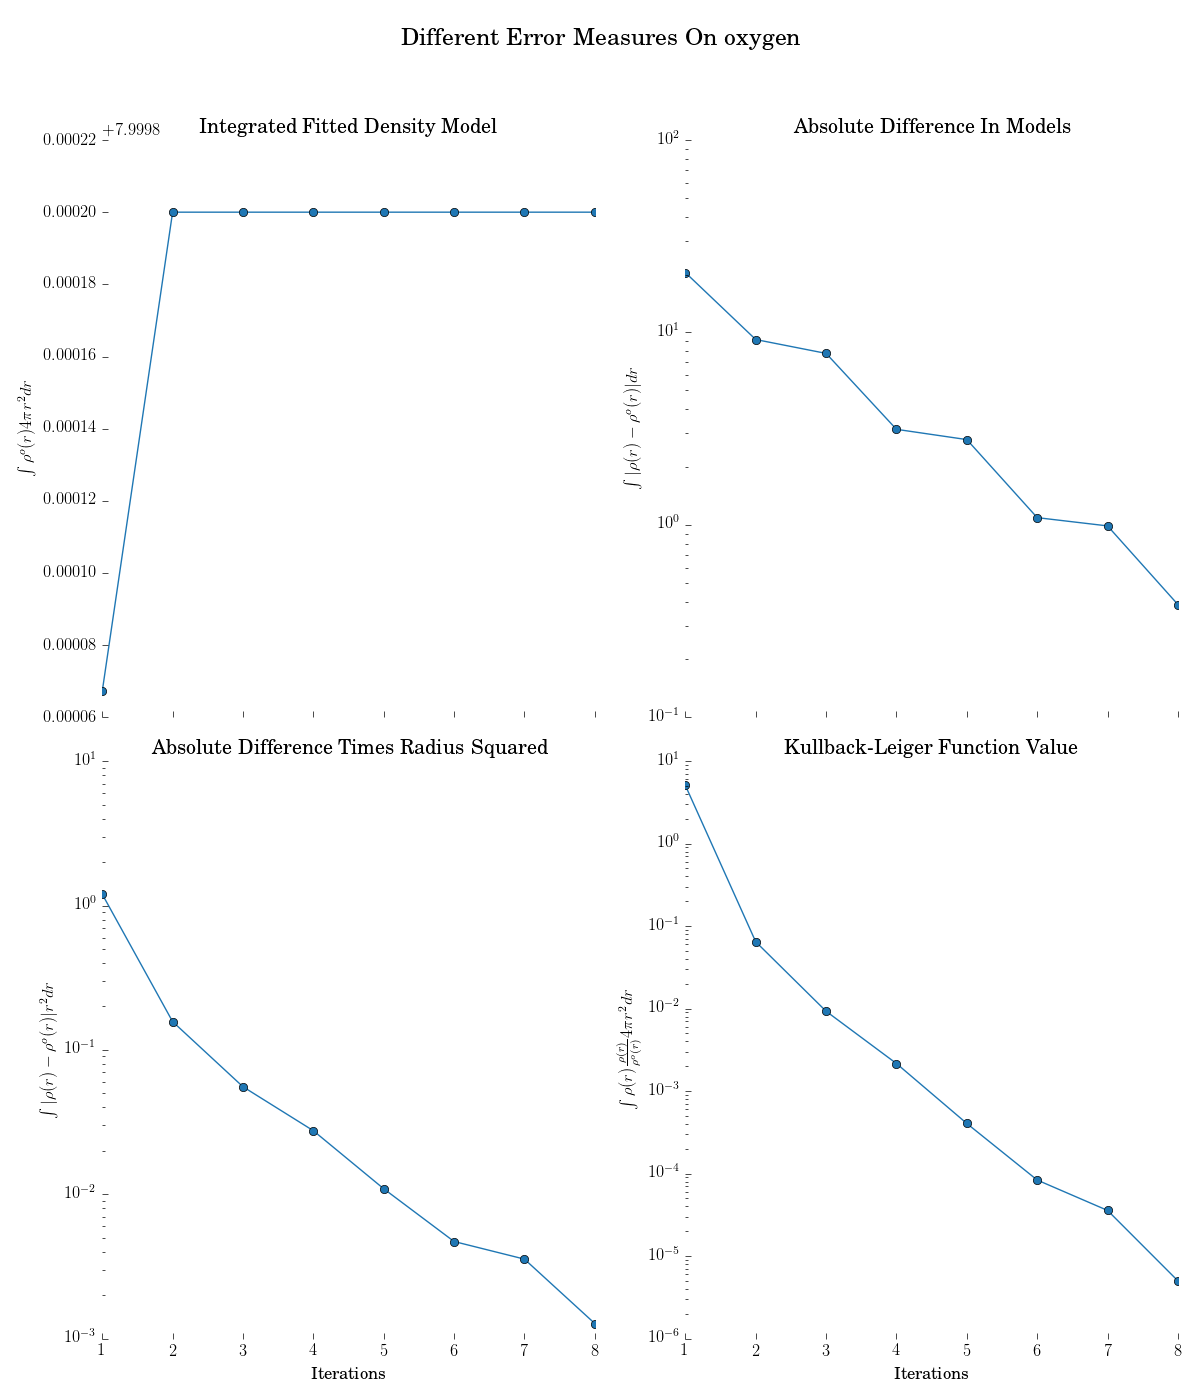
\includegraphics[scale=0.32]{results_original/o/error_plot_using_greedy-mbis.png}}
\fbox{\includegraphics[scale=0.32]{results_original/f/error_plot_using_greedy-mbis.png}}\\
\fbox{\includegraphics[scale=0.32]{results_original/ne/error_plot_using_greedy-mbis.png}}\\

\subsection{Results\textunderscore Redundancies Plots}
\fbox{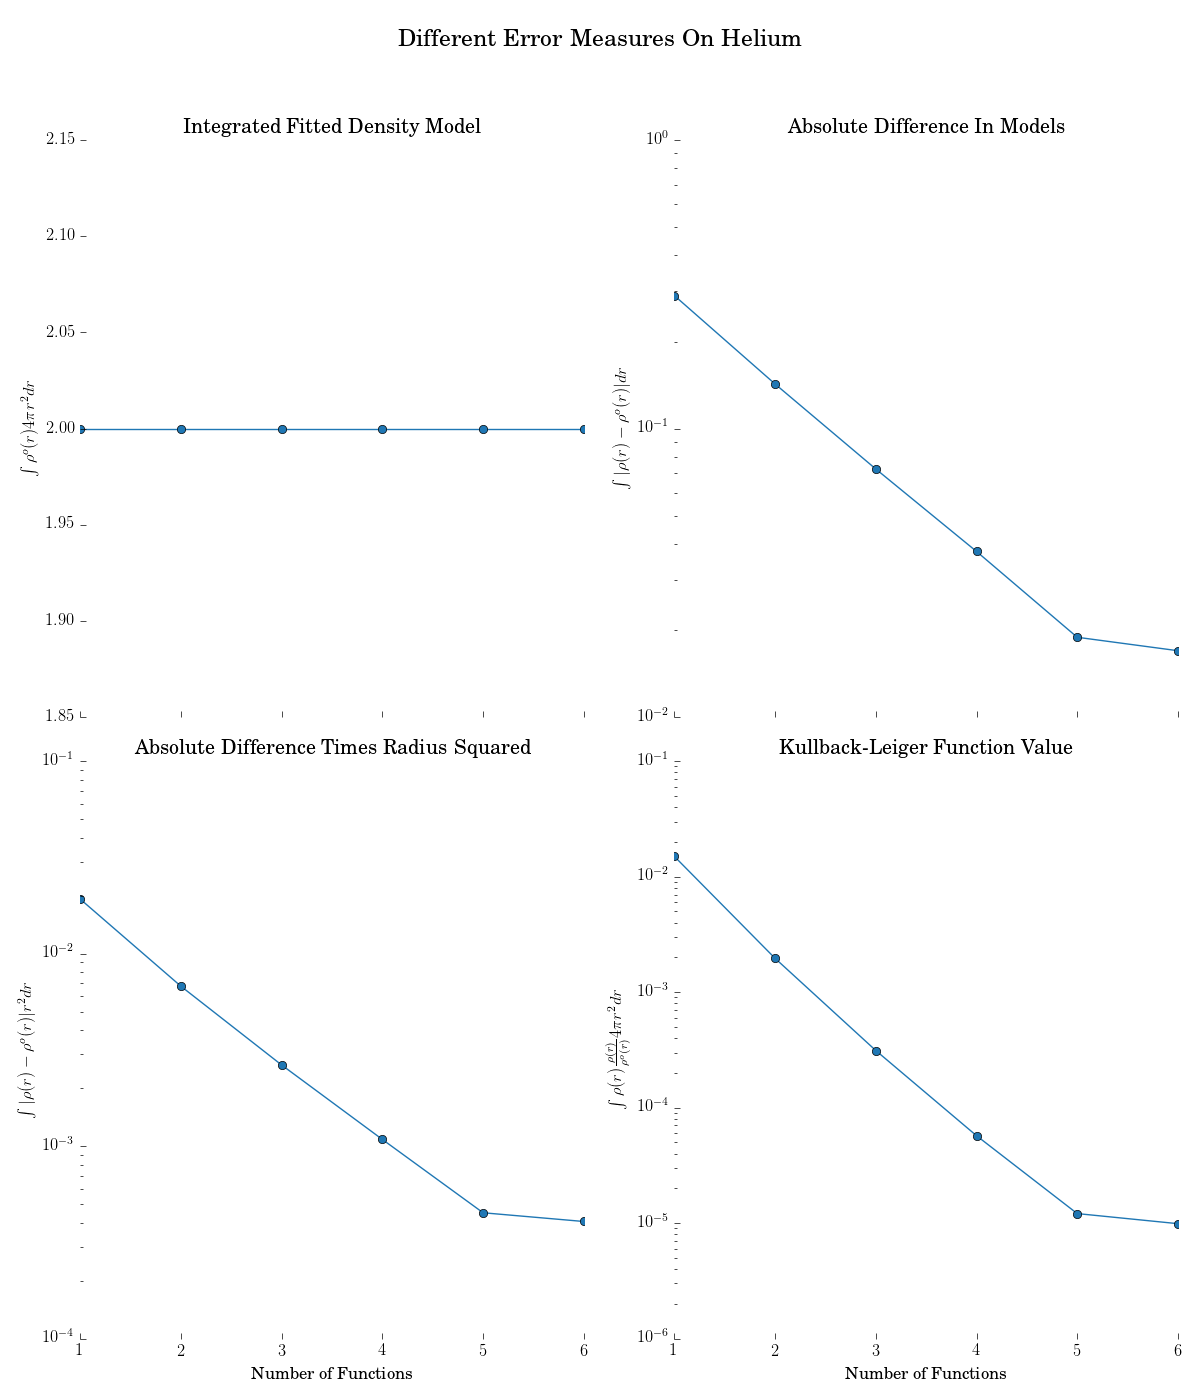
\includegraphics[scale=0.32]{results_redudancies/he/error_plot_using_greedy-mbis.png}}
\fbox{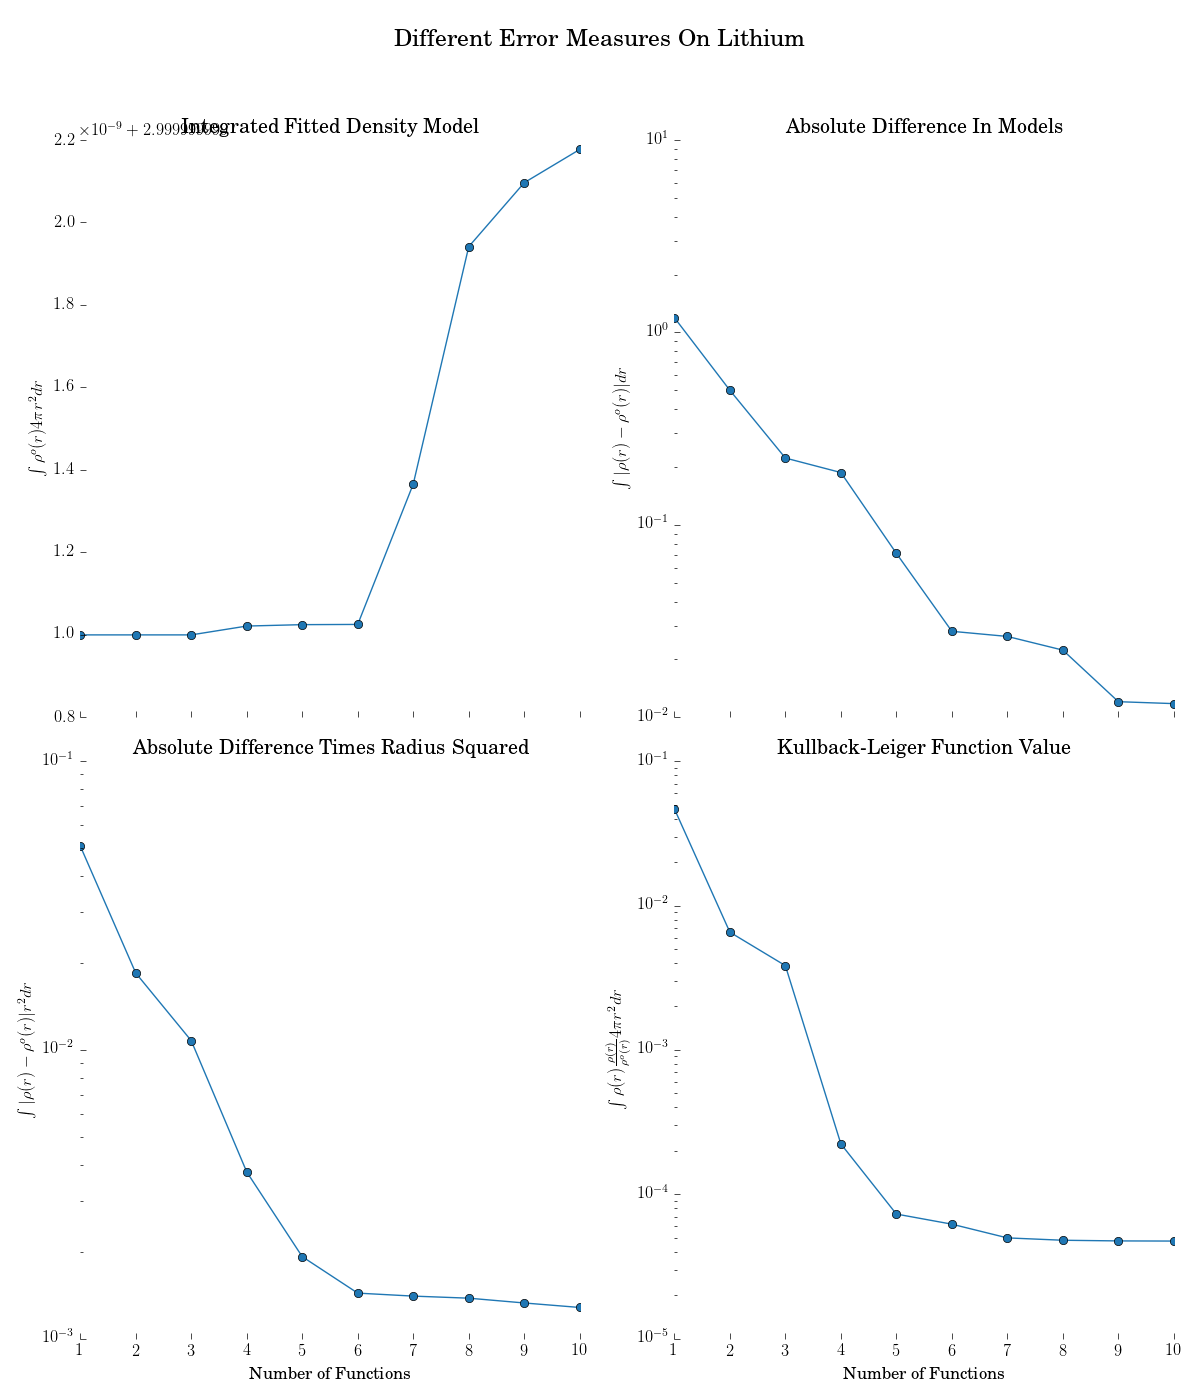
\includegraphics[scale=0.32]{results_redudancies/li/error_plot_using_greedy-mbis.png}} \\
\fbox{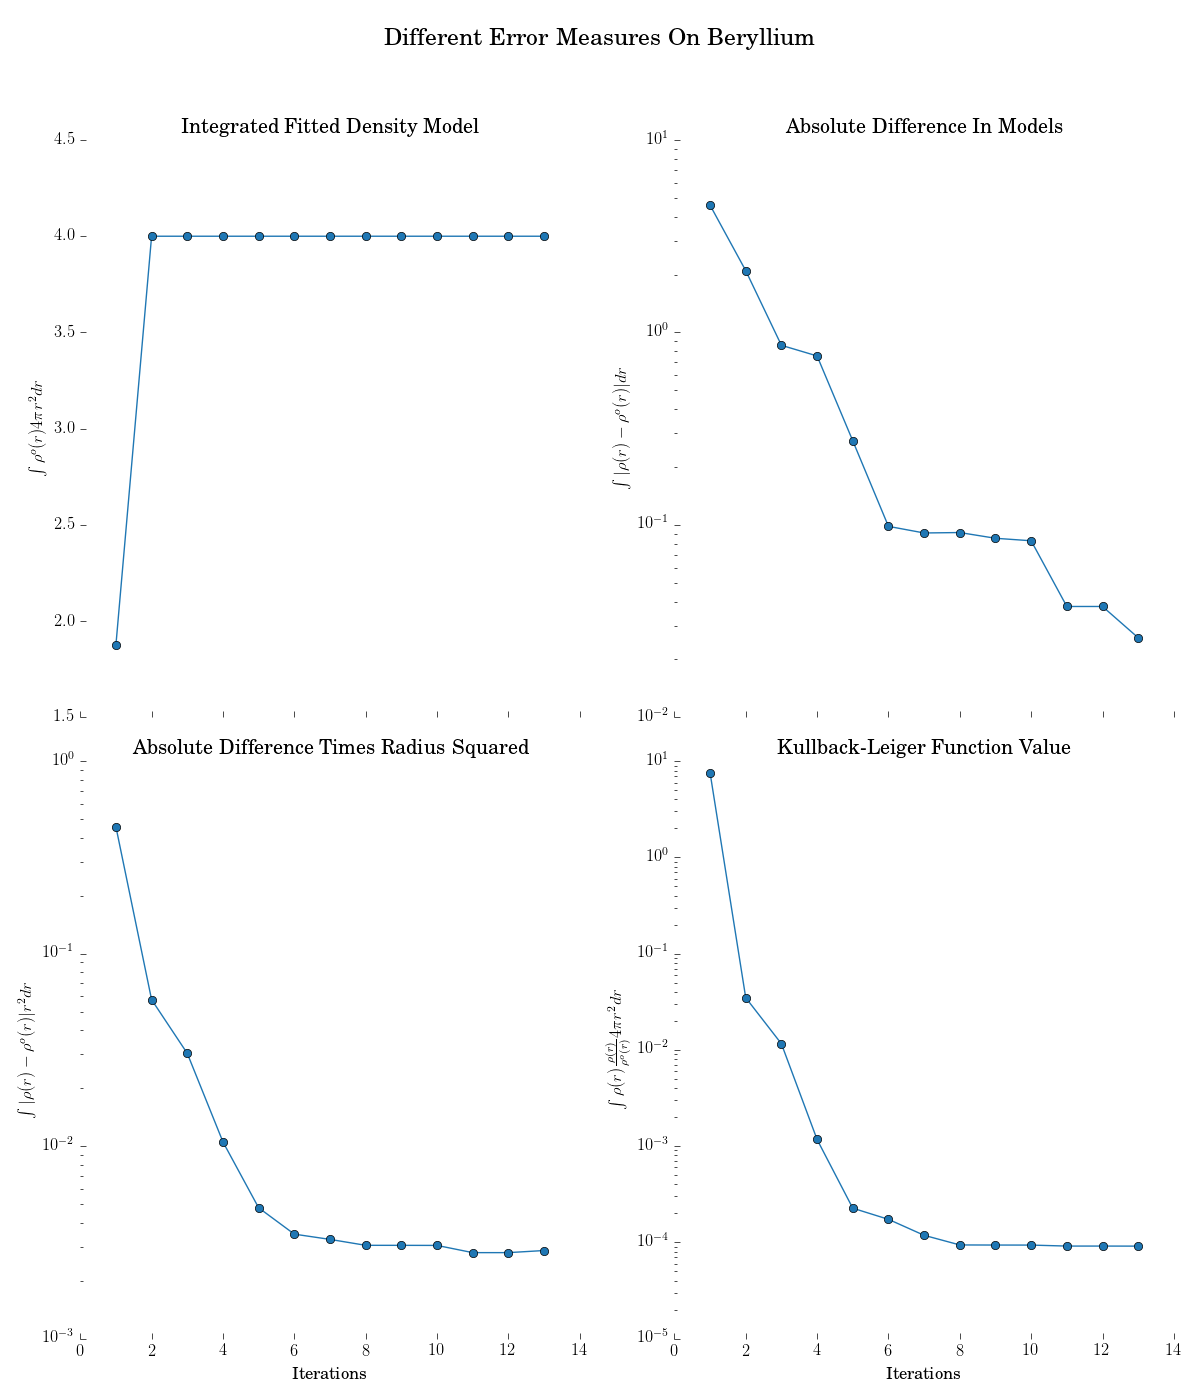
\includegraphics[scale=0.32]{results_redudancies/be/error_plot_using_greedy-mbis.png}}
\fbox{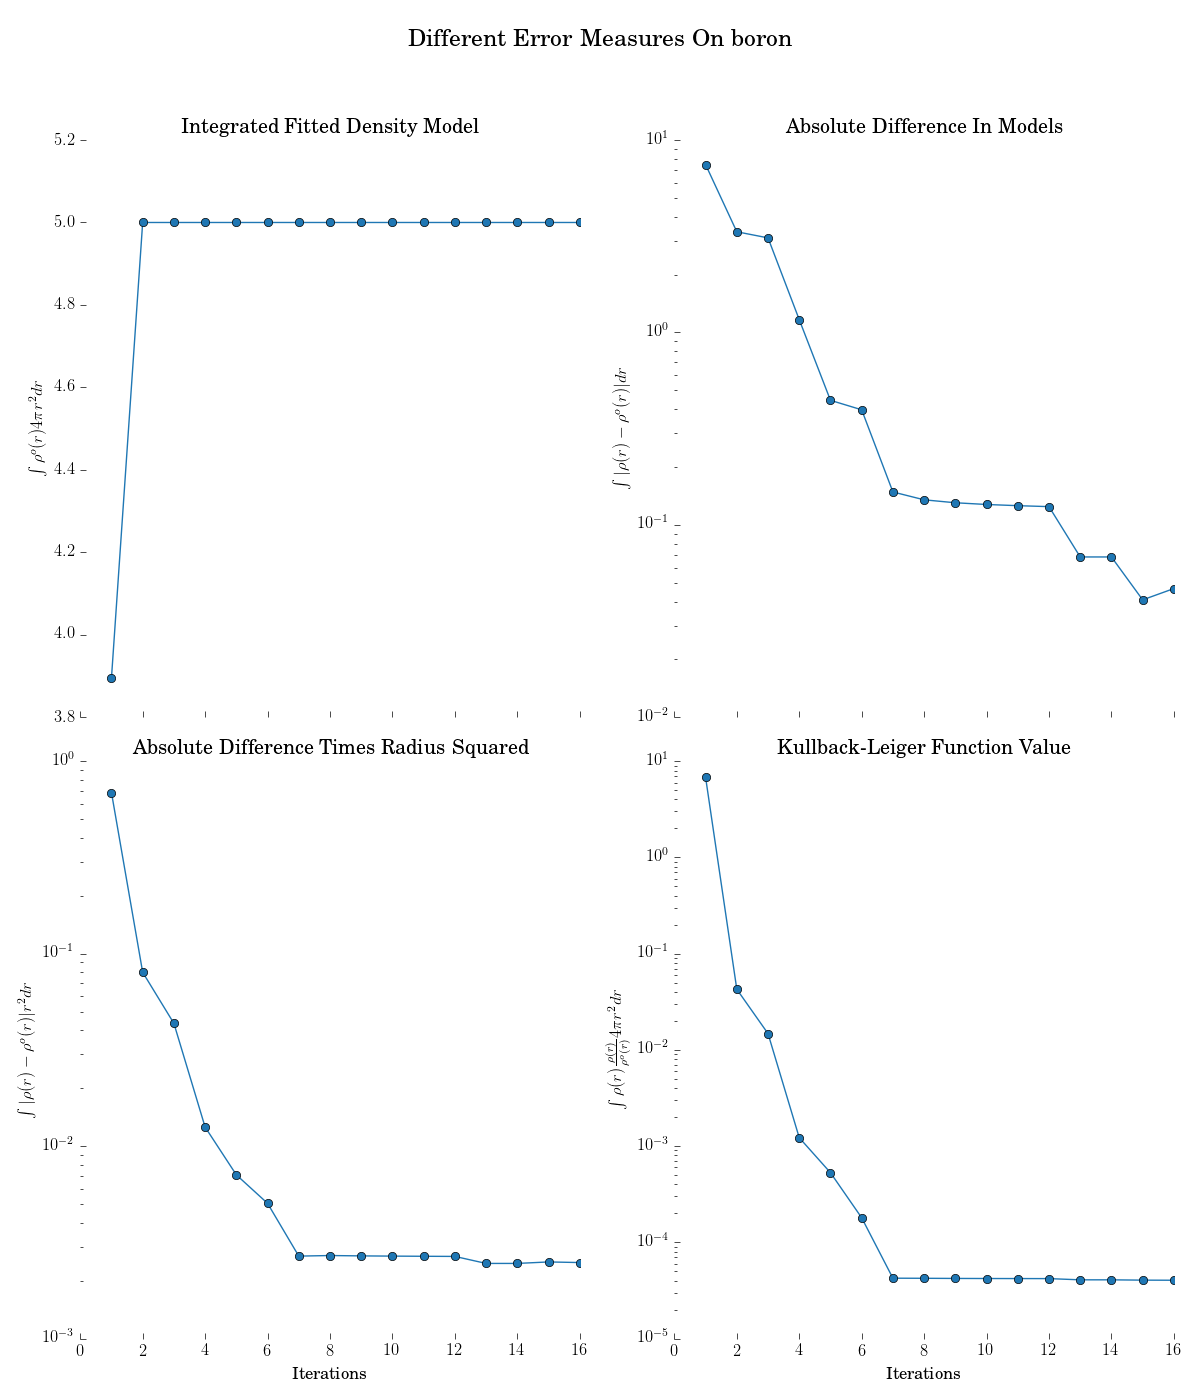
\includegraphics[scale=0.32]{results_redudancies/b/error_plot_using_greedy-mbis.png}}
\fbox{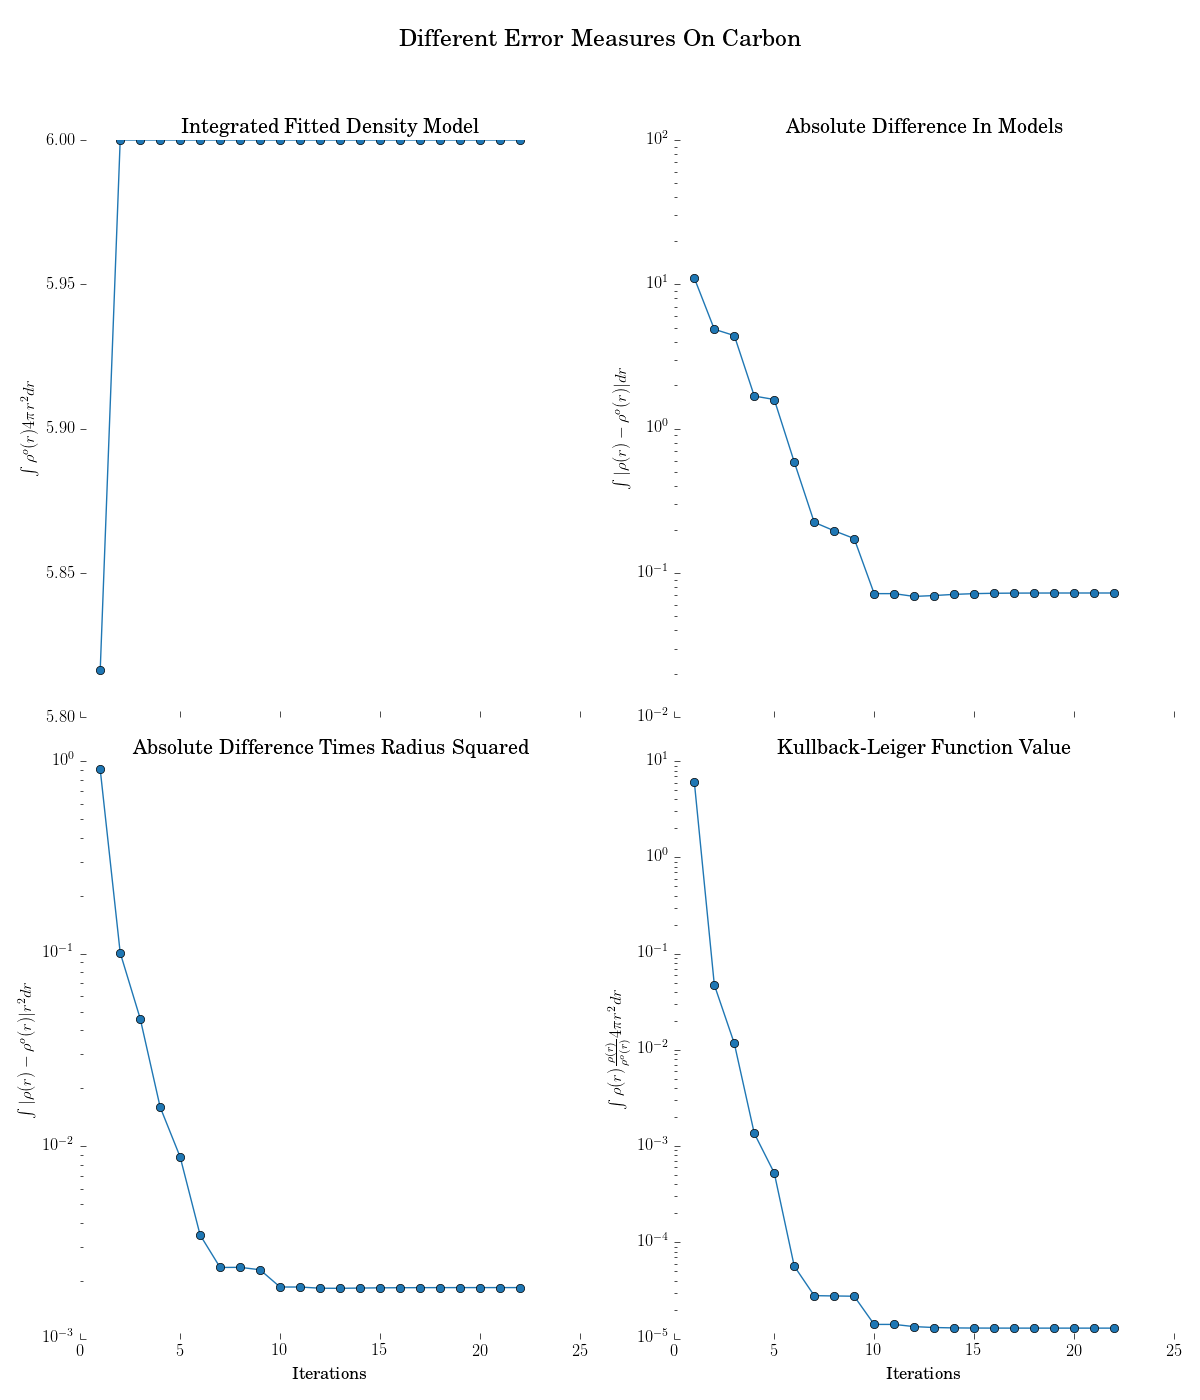
\includegraphics[scale=0.32]{results_redudancies/c/error_plot_using_greedy-mbis.png}}
\fbox{\includegraphics[scale=0.32]{results_redudancies/n/error_plot_using_greedy-mbis.png}}\\
\fbox{\includegraphics[scale=0.32]{results_redudancies/o/error_plot_using_greedy-mbis.png}}
\fbox{\includegraphics[scale=0.32]{results_redudancies/f/error_plot_using_greedy-mbis.png}}\\
\fbox{\includegraphics[scale=0.32]{results_redudancies/ne/error_plot_using_greedy-mbis.png}}\\
\end{document}
